\documentclass[journal ]{new-aiaa}
%\documentclass[conf]{new-aiaa} for conference papers
\usepackage[utf8]{inputenc}
\usepackage{textcomp}

\usepackage{graphicx}
\usepackage{amsmath}
\usepackage[version=4]{mhchem}
\usepackage{siunitx}
\usepackage{longtable,tabularx}
\setlength\LTleft{0pt} 

\usepackage{tikz} 
\usepackage{tikz-qtree}
\usetikzlibrary{trees}
\usetikzlibrary{positioning}
\usetikzlibrary{arrows.meta, calc, quotes}
\usepackage{float}
\usepackage{subcaption}
\usepackage{enumitem}
\usepackage{makecell}

\usepackage[export]{adjustbox}

\usepackage{multirow}

\usetikzlibrary{calc}

\DeclareRobustCommand{\AlphaCaption}[1]{%
  \ensuremath{\boldsymbol{\alpha}\mathbf{=#1}^{\boldsymbol{\circ}}}%
}
\DeclareRobustCommand{\DeltaCaption}[1]{%
  \ensuremath{\boldsymbol{\delta}\mathbf{=#1}^{\boldsymbol{\circ}}}%
}
\DeclareRobustCommand{\GammaCaption}[1]{%
  \ensuremath{\boldsymbol{\Gamma}\mathbf{=#1}^{\boldsymbol{\circ}}}%
}

\DeclareRobustCommand{\AlphaSimple}[1]{%
  \ensuremath{\alpha=#1^\circ}%
}
\DeclareRobustCommand{\DeltaSimple}[1]{%
  \ensuremath{\delta=#1^\circ}%
}
\DeclareRobustCommand{\GammaSimple}[1]{%
  \ensuremath{\Gamma=#1^\circ}%
}

\DeclareRobustCommand{\DeltaIn}[2]{
    \ensuremath{\delta \in [#1^\circ, #2^\circ]}
}

% Include an image and draw masking rectangles over it.
% Coordinates are normalized:
% x = 0 left, x = 1 right
% y = 0 bottom, y = 1 top
\newcommand{\MaskedImage}[3][]{%
\begin{tikzpicture}
    \node[anchor=south west, inner sep=0] (img) at (0,0)
        {\includegraphics[#1]{#2}};
    \begin{scope}[x={(img.south east)}, y={(img.north west)}]
        #3
    \end{scope}
\end{tikzpicture}%
}

% Rectangle from lower-left corner (x1,y1) to upper-right corner (x2,y2)
\newcommand{\maskrect}[5][white]{%
    \fill[#1] (#2,#3) rectangle (#4,#5);
}

% Rectangle using lower-left corner plus width and height
\newcommand{\maskrectwh}[5][white]{%
    \pgfmathsetmacro{\xr}{#2 + #4}
    \pgfmathsetmacro{\yt}{#3 + #5}
    \fill[#1] (#2,#3) rectangle (\xr,\yt);
}

% Rectangle using top-left corner plus width and height
% Useful if you think in image-editor coordinates.
\newcommand{\maskrecttl}[5][white]{%
    \pgfmathsetmacro{\xr}{#2 + #4}
    \pgfmathsetmacro{\yb}{1 - (#3 + #5)}
    \pgfmathsetmacro{\yt}{1 - #3}
    \fill[#1] (#2,\yb) rectangle (\xr,\yt);
}

\newcommand{\red}[1]{\textcolor{red}{#1}}
\newcommand{\blue}[1]{\textcolor{blue}{#1}}




\title{Multi-fidelity characterization of a positively swept tailplane with full-span control surface}

\author{Andrea Rausa\footnote{PhD, Department of Aerospace Science and Technology, Corresponding Author, andrea.rausa@polimi.it}, Giulio Gori\footnote{Associate Professor, Department of Aerospace Science and Technology}, Alex Zanotti \footnote{Associate Professor, Department of Aerospace Science and Technology}, Giuseppe Gibertini \footnote{Associate Professor, Department of Aerospace Science and Technology}, Alberto Guardone \footnote{Full Professor, Department of Aerospace Science and Technology}, and Franco Auteri \footnote{Full Professor, Department of Aerospace Science and Technology}}
\affil{Politecnico di Milano, Department of Aerospace Science and Technology, Milano, Italy, 20154}

\begin{document}

\maketitle

\begin{abstract}
This work presents a multi-fidelity numerical--experimental investigation of a positively swept, zero-dihedral tailplane equipped with a full-span trailing-edge control surface.
Wind tunnel measurements are compared with a nonlinear lifting-line model and three-dimensional Reynolds-averaged Navier--Stokes simulations over a broad range of incidence and full-span control-surface deflection.
The analysis is organized by aerodynamic regime to distinguish attached flow, control-surface separation, main-surface stall, and post-stall behavior.
Both numerical methods reproduce the main lift trends in attached and weakly nonlinear conditions, but the lifting-line model shows increasing discrepancies in pitching moment, control effectiveness, and separated-flow regimes.
The Reynolds-averaged Navier--Stokes simulations reproduce the main observed separation patterns, although the computed lift drop is more abrupt than in the experiment.
Surface-flow visualizations show extensive separation at or shortly after the experimental maximum-lift incidence, consistent with a progressive development of separation, whereas at the lower deflections the simulated fixed-surface flow remains largely attached up to maximum lift and then separates abruptly.
The comparison identifies the regimes in which each fidelity level remains informative and suggests which modeling assumptions may limit its accuracy for the swept tailplane studied.
\end{abstract}







\section{Introduction}
\label{sec:introduction}

The horizontal tailplane contributes to aircraft stability, control, maneuvering, and trim. Its aerodynamic response must be predicted over the incidence and control-deflection ranges required in service, including conditions beyond attached flow. This is particularly challenging for unconventional rear-end configurations, whose geometry may be constrained by structural requirements, propulsion integration, or packaging.

In preliminary design, control effectiveness is often described by the derivatives \(C_{L,\delta}=\partial C_L/\partial\delta\) and \(C_{M_y,\delta}=\partial C_{M_y}/\partial\delta\), where \(C_L\) and \(C_{M_y}\) are the lift and pitching-moment coefficients and \(\delta\) is the control deflection. These derivatives are evaluated at a fixed incidence \(\alpha\).
Treating these derivatives as constants assumes that the aerodynamic-coefficient increments are proportional to deflection over the operating range considered.
Although this approximation is effective at small incidence and small deflection, its validity deteriorates when separation develops over the control surface.

A full-span trailing-edge control surface can be particularly sensitive to this behavior because its deflection changes the effective camber and pressure distribution along the complete tailplane span. 
Control-surface separation may consequently alter the global lift and pitching moment before the main lifting surface reaches its conventional stall condition.

The influence of geometry and control deflection on these effects has long been examined experimentally. In classical horizontal-tail investigations, \citet{Dods1948} established the principal effects of sweep, aspect ratio, taper, and elevator deflection on lift, pitching moment, control effectiveness, and hinge moment.
\citet{PurserSpearman1951} also demonstrated through experiments on swept-back, swept-forward, and yawed wings that planform geometry modifies the spanwise circulation distribution and the progression of stall.
These investigations provide a fundamental basis for interpreting swept-tail aerodynamics, but their configurations, airfoil sections, Reynolds numbers, and measurement techniques differ from those relevant to contemporary numerical validation studies.

Sweep affects both inviscid loading and boundary-layer development on a finite lifting surface. 
The component of the external flow parallel to the leading edge produces spanwise transport and can modify the local separation behavior at the root and tip. 
These three-dimensional effects are particularly relevant to aerodynamic models that estimate finite-wing loading from two-dimensional sectional characteristics: the stall progression of the complete surface cannot, in general, be inferred directly from the sectional profile alone.
When a control surface is deflected, the interaction between sweep-induced crossflow and the adverse pressure gradient downstream of the hinge line introduces a further source of three-dimensionality. 
The resulting spanwise variations in loading and separation affect the integrated control response. Global effectiveness may therefore vary with incidence and deflection amplitude, rather than being represented by a single constant derivative.

Predicting this response during design requires a balance between representing the relevant flow mechanisms and limiting computational cost. Low-order aerodynamic methods remain indispensable during conceptual and preliminary design because they permit large geometrical and operating spaces to be investigated at limited computational cost.
Classical lifting-line theory, developed by \citet{Prandtl1921}, represents a finite lifting surface through a spanwise distribution of bound circulation and the associated trailing-vortex system.
The original linear formulation is best suited to slender lifting surfaces operating in attached flow. 
\citet{SivellsNeely1947} extended its range of applicability by introducing nonlinear sectional aerodynamic data, allowing the local section response to approach maximum lift and stall.

Subsequent lifting-line and vortex-based formulations have incorporated sweep, taper, twist, nonplanar geometry, viscous sectional data, and unsteady effects. 
\citet{SugarGabor2018} and \citet{ReidHunsaker2021} developed formulations that determine the local effective incidence from the interaction between sectional aerodynamic characteristics and the induced velocity field.
\citet{GallayGhasemiLaurendeau2014} and \citet{GoitiaLlamas2019} proposed sweep-corrected and quasi-three-dimensional formulations to approximate the differences between two-dimensional sectional behavior and the response of a finite swept wing.

Despite these developments, the predictive capability of a nonlinear lifting-line model remains tied to the validity of its sectional closure. 
Locally applied airfoil polars cannot explicitly reproduce spanwise boundary-layer transport, junction flow, tip-vortex interaction, or changes in the topology of strongly separated flow. 
Moreover, using two-dimensional post-stall characteristics may introduce an incorrect separation onset or inaccurately redistribute loading along the span. 
A model can therefore reproduce an integrated lift coefficient while retaining substantial errors in the local loading or pitching moment.
Establishing the operating range over which the sectional approximation remains adequate is therefore an important part of validating such methods.

Reynolds-averaged Navier--Stokes (RANS) methods offer a complementary description by solving the three-dimensional mean-flow conservation equations with a turbulence closure, rather than obtaining viscous loads from sectional lookup tables.
The coupled pressure and velocity fields account for three-dimensional boundary-layer development within the assumptions of the turbulence and transition models, allowing surface loading and separation patterns to be examined.
Their reliability is generally strongest in attached and mildly separated flow.
Near stall, the predicted onset and extent of separation may depend strongly on turbulence closure, laminar-to-turbulent transition modeling, grid resolution, boundary conditions, and the assumption that the flow can be represented by a steady mean solution.

A meaningful comparison of RANS calculations with wind tunnel measurements must also distinguish model-form error from differences between the numerical and experimental configurations. 
The computational model should reproduce the experimental geometry, Reynolds and Mach numbers, control setting, boundary-layer state, and relevant tunnel boundaries as closely as possible. 
Numerical verification and experimental uncertainty must be considered alongside the coefficient differences~\citep{ClarkEtAl2020}. 
The experimental uncertainty is therefore considered when evaluating the differences between numerical predictions and measurements.

The complementary capabilities of experimental measurements, high-fidelity simulations, and low-order aerodynamic models motivate a multi-fidelity approach. 
In such a framework, the inexpensive model provides broad parameter-space coverage, the higher-fidelity model provides detailed flow information, and the experiment establishes the physical reference against which discrepancies between models can be assessed~\citep{PeherstorferWillcoxGunzburger2018}. 

The Clean Sky 2 MONNALISA project was established to develop and validate this type of methodology for unconventional lifting surfaces with controls~\cite{auteri2022monnalisa}. 
The project generated an experimental and numerical database covering variations in sweep, aspect ratio, taper ratio, dihedral, angle of attack, and full-span control-surface deflection. 
Initial work addressed numerical comparisons of unconventional tail configurations~\citep{RausaEtAl2022}, experimental characterization of the boundary-layer transition state~\citep{ZanottiEtAl2022}, and Bayesian calibration of the low-order aerodynamic model~\citep{GoriEtAl2023}.

The authors subsequently documented the structure, methodologies, and contents of the complete MONNALISA database~\citep{rausa2026monnalisa}.
That study presented the full geometrical parameterization, computational and experimental procedures, database organization, and an initial comparison of the available fidelity levels. 
The comparison indicated agreement among the experimental, lifting-line, and RANS data in the approximately linear regime, with increasing discrepancies at large incidence and control deflection.
The database paper primarily documented available resources and did not provide a complete, configuration-specific analysis of control effectiveness, separation development, local loading, or numerical model validity.

The present study examines the positively swept, zero-dihedral reference tailplane across the available incidence--deflection range.
The objectives are to compare lift, drag, and pitching moment among the three methods; quantify the incidence dependence of control effectiveness; and relate the coefficient differences to control-surface separation, main-surface stall, and post-stall flow patterns.
The results are organized by aerodynamic regime so that the numerical assumptions can be assessed against both the integrated measurements and the surface-flow visualizations.

The remainder of the paper is organized as follows.
Section~\ref{sec:configuration} defines the selected geometry, operating conditions, and aerodynamic quantities.
Section~\ref{sec:methodology} summarizes the experimental and numerical methods, with detailed derivations and database procedures referred to the preceding MONNALISA publication.
Section~\ref{sec:results} presents the multi-fidelity comparison, the analysis of the governing flow mechanisms, and the regime-dependent assessment of the numerical methods.













\section{Configuration and Operating Conditions}
\label{sec:configuration}

\subsection{Tailplane geometry}
\label{sec:geometry}

The configuration is the positively swept reference tailplane of the MONNALISA database~\citep{rausa2026monnalisa}, with zero dihedral, a trapezoidal planform, a quarter-chord sweep of $30^\circ$, an aspect ratio of $5$, and a taper ratio of $0.4$.
In this convention, positive sweep means the tip is downstream of the root. 
The aspect ratio refers to the equivalent full-span planform. The semispan is $b_s=1.6~\mathrm{m}$, the semispan reference area is $S_{\mathrm{ref}}=1.024~\mathrm{m^2}$, and the mean aerodynamic chord is $\bar{c}=0.679184~\mathrm{m}$.

The tailplane uses a single symmetric airfoil, scaled to the local chord along the full span.
Its maximum thickness is $9\%$ of the local chord. 
A control surface is located at the trailing edge and extends over the full semispan.
The control surface rotates about a hinge located at $70\%$ of the local chord. 
Its chord is therefore $30\%$ of the local tailplane chord.
The measured control settings are \(\delta \in \{0^\circ,10^\circ,20^\circ,30^\circ,34^\circ\}\); the numerical counterparts use \(35^\circ\) for the largest setting.
%
Positive control deflection corresponds to the trailing edge rotating downward. Fig.~\ref{figure:PlanformDefinition} illustrates the geometrical parameters and sign conventions.
%
\begin{figure}
\begin{minipage}[ht]{0.45\textwidth}
    \begin{subfloat}[]{
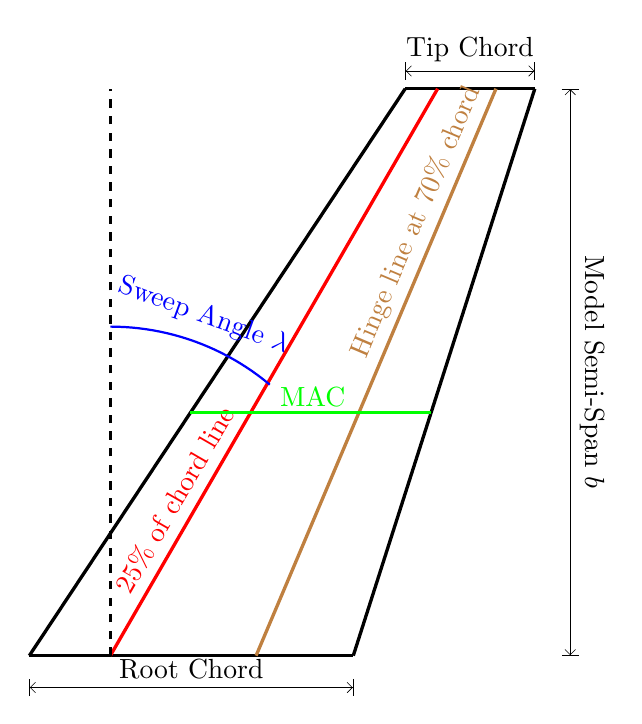
\begin{tikzpicture}[scale=0.45, auto = left,
measure/.style = {very thin,
        {Bar[width=2.2mm]Straight Barb[]}-%
        {Straight Barb[]Bar[width=2.2mm]},
            },
every label/.append style = {font=\footnotesize}]

        \coordinate (LE_R) at ( 0, 0, 0 );
        \coordinate (TE_R) at ( 9.1428, 0, 0 );
        \coordinate (LE_T) at ( 10.609, 16, 0 );
        \coordinate (TE_T) at ( 14.266, 16, 0 );
        \draw[very thick,black] (LE_R) -- (TE_R);
        \draw[very thick,black] (LE_T) -- (TE_T);
        \draw[very thick,black] (LE_T) -- (LE_R);
        \draw[very thick,black] (TE_R) -- (TE_T);
        
        \coordinate (AC_R) at ( 2.28575, 0, 0 );
        \coordinate (AC_T) at ( 11.5233, 16, 0 );
        \draw[very thick,red] (AC_R) -- (AC_T);
        
        \coordinate (Text_Sweep) at ( 4.6, 4.1, 0 );
        \node [rotate=60,anchor=south] at (Text_Sweep) {\textcolor{red}{25\% of chord line}}; 
        
        \coordinate (AC_RT) at ( 2.28575, 16, 0 );
        \draw[very thick,black,dashed] (AC_R) -- (AC_RT);

        \draw [blue,thick,domain=50:90] plot ({2.28575+7*cos(\x)}, {2.28575+7*sin(\x)});
        
        \coordinate (Text_Sweep_Sym) at ( 4.7, 9, 0 );
        \node [rotate=-20,anchor=south] at (Text_Sweep_Sym) {\textcolor{blue}{Sweep Angle $\lambda$}}; 

        \coordinate (H_R) at ( 6.4, 0, 0 );
        \coordinate (H_T) at ( 13.17, 16, 0 );
        \draw[very thick,brown] (H_R) -- (H_T);
        
        \coordinate (Text_Hinge) at ( 11.5, 12, 0 );
        \node [rotate=67,anchor=south] at (Text_Hinge) {\textcolor{brown}{Hinge line at 70\% chord}}; 
        
        \coordinate (TE_TR) at ( 14.266, 0, 0 );
        \draw[measure]  ($(TE_T)!10mm!90:(TE_TR)$) to [sloped,"Model Semi-Span $b$"] ($(TE_TR)!10mm!-90:(TE_T)$);
        
        \draw[measure]  ($(LE_T)!5mm!90:(TE_T)$) to [sloped,"Tip Chord"] ($(TE_T)!5mm!-90:(LE_T)$);

        \coordinate (LE_MAC) at ( 4.547, 6.857, 0 );
        \coordinate (TE_MAC) at ( 11.339, 6.857, 0 );
        \draw[very thick,green] (LE_MAC) -- (TE_MAC);
        \coordinate (Text_MAC) at ( 8, 7.3, 0 );
        \node [] at (Text_MAC) {\textcolor{green}{MAC}}; 
        
        \draw[measure]  ($(LE_R)!9mm!-90:(TE_R)$) to [sloped,"Root Chord"] ($(TE_R)!9mm! 90:(LE_R)$);
        
    \end{tikzpicture}
}
\end{subfloat}
\end{minipage}
\quad
\begin{minipage}[ht]{0.45\textwidth}
\begin{subfloat}[]{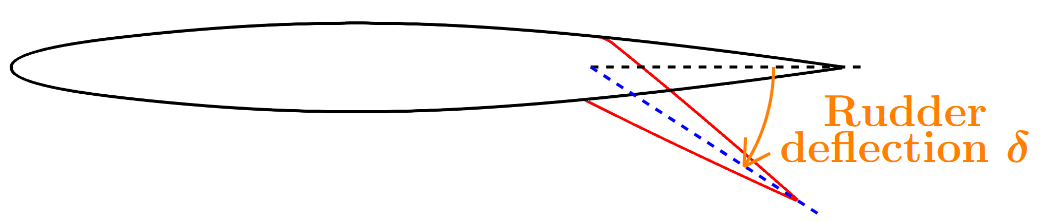
\includegraphics[width=1\textwidth]{FlapDeflection.png}\label{figure:PlanformDefinition:Rudder}}
\end{subfloat}
\begin{subfloat}[]{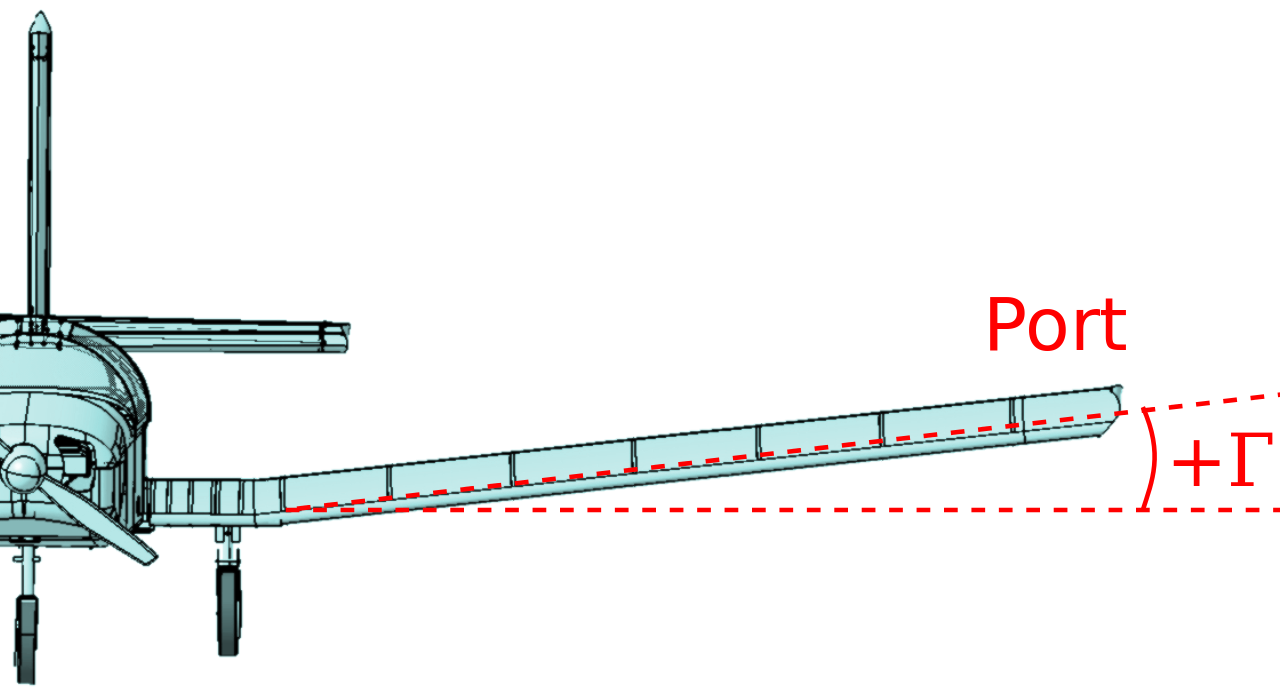
\includegraphics[width=1\textwidth]{Aircraft_dihedral_angle.png}\label{figure:PlanformDefinition:Dihedral}}
\end{subfloat}
\end{minipage}
\caption[Visual definition of geometric parameters]{Planform definition of a trapezoidal lifting surface \cite{rausa2026monnalisa}: \textbf{(a)} in-plane parameters, \textbf{(b)} control surface deflection definition \red{perché rudder e non elevator?} \blue{C'è stata una lunga discussione con Wolfgang per la sottomissione del database su ERCOFTAC ed alla fine abbiamo deciso di chiamarlo rudder, o ancora meglio control surface}, \textbf{(c)} dihedral angle.}
\label{figure:PlanformDefinition}
\end{figure}

%
The pitching moment is considered positive nose up.
%
%
% \begin{table}[htbp]
% \centering
% \caption{Principal geometrical parameters of the investigated
% tailplane.}
% \label{tab:geometry}
% \begin{tabular}{lccc}
% \hline
% \hline
% Parameter & Symbol & Value & Unit 
% \\
% \hline
% Quarter-chord sweep angle
% & $\lambda$ & $30.0$ & deg 
% \\
% Dihedral angle
% & $\Gamma$ & $0.0$ & deg 
% \\
% Aspect ratio
% & $AR$ & $5.0$ & -- 
% \\
% Taper ratio
% & $\tau$ & $0.4$ & -- 
% \\
% Model semispan
% & $b_s$ & $1.6$ & m 
% \\
% Reference area
% & $S_{\mathrm{ref}}$ & $1.024$ & m$^2$ 
% \\
% Mean aerodynamic chord
% & $\bar{c}$ & $0.679184$ & m 
% \\
% Thickness-to-chord ratio
% & $t/c$ & $0.09$ & -- 
% \\
% Hinge-line position
% & $x_h/c$ & $0.70$ & -- 
% \\
% Control-surface span ratio
% & $b_{\mathrm{cs}}/b_s$ & $1.0$ & -- 
% \\
% \hline
% \hline
% \end{tabular}
% \end{table}
%
%
%
The aerodynamic coefficients are defined as
%
\begin{equation}
C_L =
\frac{L}{q_\infty S_{\mathrm{ref}}},
\qquad
C_D =
\frac{D}{q_\infty S_{\mathrm{ref}}},
\qquad
C_{M_y} =
\frac{M_y}
{q_\infty S_{\mathrm{ref}}\bar{c}},
\label{eq:aero_coefficients}
\end{equation}
%
where $L$, $D$, and $M_y$ are lift, drag, and pitching moment, and $q_\infty=\rho_\infty V_\infty^2/2$ is the freestream dynamic pressure. The quantities $\rho_\infty$ and $V_\infty$ are freestream density and speed.
The pitching moment is evaluated about a spanwise axis at the aerodynamic-center coordinate \(x_{AC}\), estimated separately for each dataset from its undeflected force and moment slopes in the approximately linear incidence range.
For each dataset, this reference point is retained for all control-surface settings so that changes in \(C_{M_y}\) reflect changes in the aerodynamic loading rather than changes in the moment origin.

The nondimensional spanwise coordinate is defined as
%
\begin{equation}
\eta = \frac{y}{b_s},
\qquad
0 \leq \eta \leq 1,
\label{eq:span_coordinate}
\end{equation}
%
with $\eta=0$ at the model root and $\eta=1$ at the tip.





\subsection{Operating conditions and test matrix}
\label{sec:operating_conditions}

The numerical simulations use the nominal Mach and Reynolds numbers of the wind tunnel tests.
The Mach number is $M_\infty=0.147$, and the Reynolds number based on model semispan is
%
\begin{equation}
Re_{b_s}
=
\frac{\rho_\infty V_\infty b_s}
{\mu_\infty}
=
5.5\times10^6.
\label{eq:reynolds}
\end{equation}
%
Here $\mu_\infty$ is the freestream dynamic viscosity. The nominal freestream temperature is $300~\mathrm{K}$, and the wind tunnel turbulence intensity is below $0.1\%$.

In the wind tunnel, the angle of attack ranges from $-25^\circ$ to $25^\circ$, in $2^\circ$ increments between $-24^\circ$ and $24^\circ$, with final steps of $1^\circ$. The numerical calculations cover $-26^\circ$ to $26^\circ$ in increments of $2^\circ$. This range includes the attached linear regime, control-surface separation, main-surface stall, and deep post-stall conditions. 
% The complete nominal test matrix is summarized in Table~\ref{tab:test_matrix}.

% \begin{table}[htbp]
% \centering
% \caption{Nominal operating conditions and investigated variables.}
% \label{tab:test_matrix}
% \begin{tabular}{lcc}
% \hline
% \hline
% Quantity & Value or range & Increment 
% \\
% \hline
% Mach number, $M_\infty$
% & $0.147$ & -- 
% \\
% Semispan Reynolds number, $Re_{b_s}$
% & $5.5\times10^6$ & -- 
% \\
% Freestream temperature, $T_\infty$
% & $300~\mathrm{K}$ & -- 
% \\
% Turbulence intensity, $TI_\infty$
% & $\leq 0.1\%$ & -- 
% \\
% Angle of attack, $\alpha$
% & $[-26^\circ,26^\circ]$ & $2^\circ$ 
% \\
% Control deflection, $\delta$
% & ${0^\circ,10^\circ,20^\circ,30^\circ,34^\circ}$
% & discrete 
% \\
% Dihedral angle, $\Gamma$
% & $0^\circ$ & -- 
% \\
% \hline
% \hline
% \end{tabular}
% \end{table}

Surface-flow fields are examined at representative operating points selected to illustrate control-surface separation, main-surface stall, and post-stall load redistribution.










\section{Experimental and Numerical Methodology}
\label{sec:methodology}

The experimental and numerical data analyzed in this work are part of the MONNALISA database. The authors\textquotesingle{} preceding database paper~\citep{rausa2026monnalisa} describes the complete test campaign, numerical formulations, grid-generation procedure, wind tunnel corrections, and database organization. This section summarizes the information needed to interpret the configuration-specific comparison and highlights the assumptions that affect the validation results.

\subsection{Wind tunnel experiments}
\label{sec:wind_tunnel}

The experiments were performed in the Low Turbulence Test Section of the large closed-circuit wind tunnel at Politecnico di Milano. The effective test section was approximately $4~\mathrm{m}$ wide, $3.49~\mathrm{m}$ high, and $6~\mathrm{m}$ long. A dummy floor was installed to enclose the model support, the aerodynamic balance, and the control-surface actuation mechanism. The tailplane was mounted as a vertical semispan model, and the angle of attack was varied by rotating the base of the supporting frame.

The installation is shown in Fig.~\ref{fig:wind_tunnel_installation}.
\begin{figure}[htbp]
    \centering
    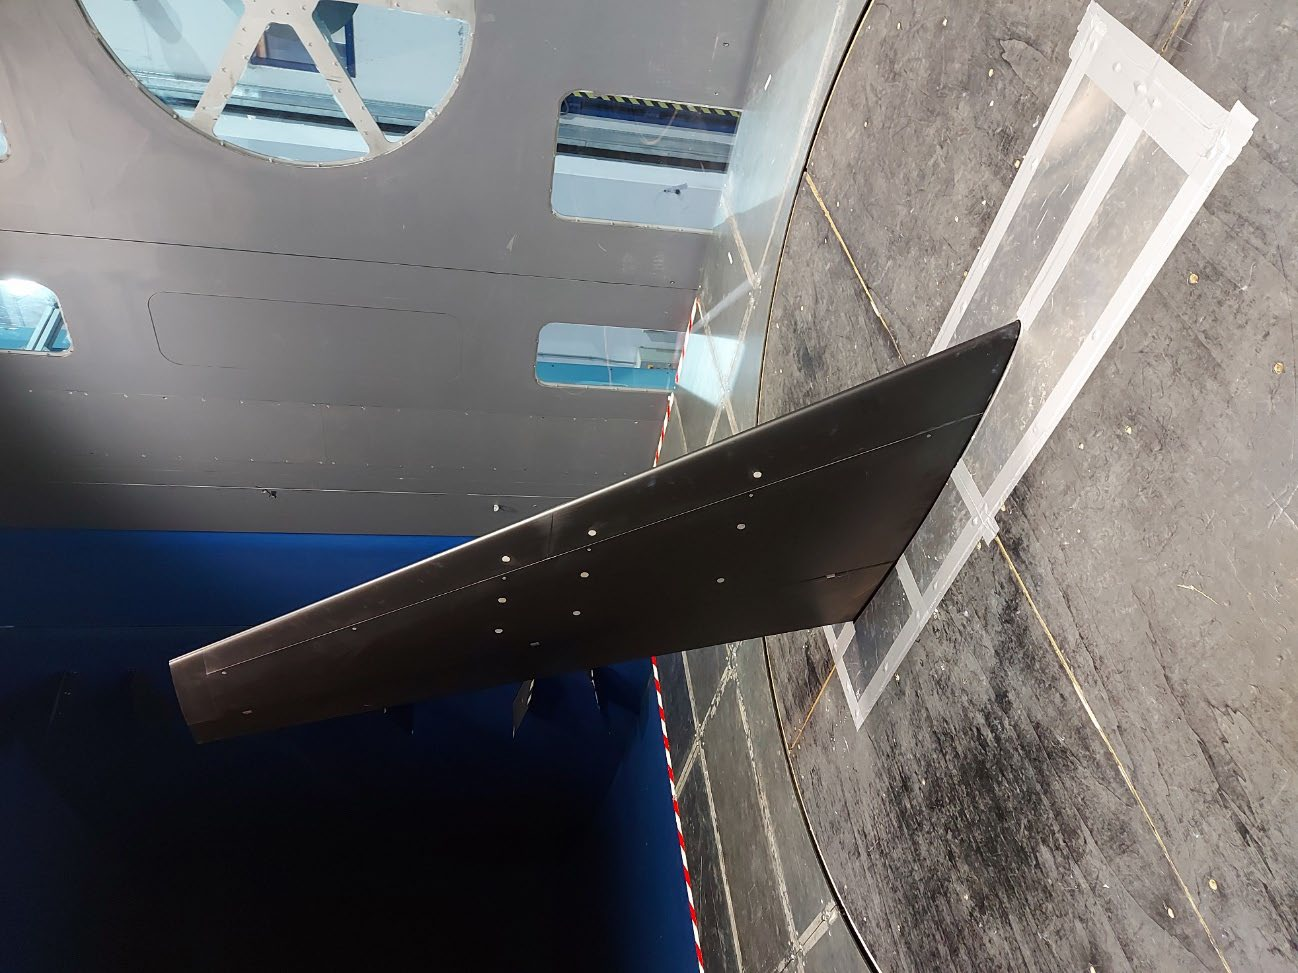
\includegraphics[angle=-90,width=0.48\linewidth]{WindTunnelInstallation.jpg}
    \caption{Reference semispan tailplane installed vertically above the wind tunnel dummy floor.}
    \label{fig:wind_tunnel_installation}
\end{figure}

The maximum test-section velocity is approximately $55~\mathrm{m\,s^{-1}}$, and the freestream turbulence intensity is below $0.1\%$. Measurements of the total-pressure distribution showed variations within approximately $0.5\%$ of the dynamic pressure over most of the test section and below approximately $1\%$ elsewhere outside the wall boundary layers. The chamber is slightly divergent to compensate for boundary-layer growth, leaving a small residual streamwise static-pressure gradient.

The aerodynamic forces and moments were measured using an RUAG 767 strain-gauge balance installed beneath the dummy floor. The balance measured the loads acting on the complete semispan model. The measured forces and moments were nondimensionalized using the freestream dynamic pressure and the reference quantities in Eq.~\ref{eq:aero_coefficients}. The measured loads were transformed from the balance reference system to the wind-axis system before comparison with the numerical results.

The measured data were corrected for horizontal buoyancy, solid blockage, wake blockage, and the modification of the effective angle of attack produced by the test-section boundaries. The complete correction procedure is reported in the authors\textquotesingle{} database paper~\citep{rausa2026monnalisa} and follows standard low-speed wind tunnel practice~\citep{barlow1999low}. The present analysis uses the corrected aerodynamic coefficients and corrected angle of attack.

The experimental error bars are the uncertainties supplied with the database, propagated through the complete measurement and data-reduction chain, including the balance and the transformation to the wind-axis system~\citep{rausa2026monnalisa}. The pitching moment about the aerodynamic center also retains the propagated uncertainty of the fitted aerodynamic-center position.

Surface-flow visualizations are used to compare the experimental separation patterns with the RANS skin-friction lines.


\subsection{Nonlinear lifting-line model}
\label{sec:lifting_line}

The low-order predictions were obtained using the nonlinear lifting-line model implemented in DUST \citep{TUGNOLI2021106804}. A one-dimensional spanwise distribution of bound circulation represents the lifting surface. The trailing vortex system induces a velocity field that modifies the local effective incidence at each lifting-line element.

For a generic spanwise position, the effective incidence may be expressed as
%
\begin{equation}
\alpha_{\mathrm{eff}}(\eta)
=
\alpha_{\mathrm{geom}}(\eta)
-
\alpha_{\mathrm{ind}}(\eta),
\label{eq:effective_incidence}
\end{equation}
%
where $\alpha_{\mathrm{geom}}$ is the local geometric incidence and $\alpha_{\mathrm{ind}}$ is the incidence induced by the circulation and wake system. The local lift, drag, and pitching-moment coefficients are interpolated from sectional polars as functions of effective incidence, Reynolds number, Mach number, and control deflection.

The tabulated characteristics are obtained from C81 lookup tables generated by two-dimensional RANS calculations of the sectional profile. Separate sectional geometries and polars are used for the different control-surface deflections. Control deflection is therefore represented through the aerodynamic response of the deflected profile rather than through a prescribed linear control-effectiveness factor.
The nonlinear $\Gamma$ method determines the circulation distribution by enforcing consistency between the sectional aerodynamic data and the Kutta--Joukowski relation. Iterations continue until the circulation distribution, induced incidence, and local sectional loads are mutually consistent.

Because the tailplane is swept, the two-dimensional sectional characteristics are modified using the quasi-three-dimensional correction proposed by \citet{GoitiaLlamas2019}. The correction combines the conventional transformation of the sectional data with a span-dependent modification of the effective sweep:
%
\begin{equation}
\lambda_{\mathrm{eff}}(\eta)
=
\lambda_{\mathrm{loc}}(\eta)
\kappa(\eta),
\label{eq:effective_sweep}
\end{equation}
%
where $\lambda_{\mathrm{loc}}$ is the local geometric sweep and $\kappa(\eta)$ contains empirical root- and tip-region corrections. The functional form of the correction is given by \citet{GoitiaLlamas2019}; its application in MONNALISA is described in the authors\textquotesingle{} database paper~\citep{rausa2026monnalisa}.

The lifting-line solution provides global aerodynamic coefficients and spanwise distributions of circulation and sectional loads at a small computational cost. Two-dimensional viscous effects are included through the sectional polars, but the method does not resolve the three-dimensional boundary-layer field or separated-flow topology. Its ability to reproduce control-surface stall and main-surface separation depends on the sectional polars and on how well the sweep correction represents the actual spanwise redistribution of loading. The comparison in Section~\ref{sec:results} examines the consequences of these sectional assumptions.

\subsection{Reynolds-averaged Navier--Stokes model}
\label{sec:rans}

The higher-fidelity numerical predictions were obtained using the SU2 open-source computational framework \citep{palacios2013stanford}. The steady compressible RANS equations were discretized using a vertex-centered finite-volume method on an unstructured median-dual grid.

Convective fluxes were evaluated using the Roe approximate Riemann solver~\citep{Roe1981}. Second-order spatial accuracy was obtained using MUSCL reconstruction~\citep{van1979towards}, with a Venkatakrishnan limiter~\citep{venkatakrishnan1993accuracy} to reduce spurious oscillations in regions with strong solution gradients. An implicit Euler pseudo-time-integration procedure advanced the equations toward a steady solution~\citep{palacios2013stanford}.

Turbulence closure was provided by the Spalart--Allmaras one-equation model \citep{spalart1992sa}. Laminar-to-turbulent transition was represented using the algebraic Bas--Cakmakcioglu formulation \citep{cakmakcioglu2020bcm}. A transition-sensitive model is relevant because infrared measurements indicate that the boundary-layer state varies with incidence and spanwise position \citep{ZanottiEtAl2022}.

The tailplane surface was modeled as an adiabatic no-slip wall. Freestream conditions were imposed on the external far-field boundaries, and the model root was represented as a symmetry plane.

The computational meshes were generated using an automated procedure based on a parametric CAD representation and Pointwise. Anisotropic surface elements were used near the leading edge and control-surface junction, while a hex-dominant, octree-based volume mesh was used away from the wall. Additional refinement was introduced near the tail tip and along an incidence-dependent wake region. Near-wall layers were constructed to resolve the boundary layer consistently with the turbulence and transition models.

A four-level mesh study was previously performed for representative attached and separated conditions. For the zero-dihedral geometry, the nominal meshes contained approximately $10$--$13$ million grid points, depending on incidence, while the finest meshes contained up to approximately $65$ million points. Changes in the integrated lift and drag coefficients relative to the finest meshes remained below approximately $4\%$, although strictly monotonic convergence was not obtained in every case. The present comparison uses those existing solutions and the associated grid-verification evidence \citep{rausa2026monnalisa}.

Convergence was monitored using the mean variation of the lift and drag coefficients over a prescribed iteration window:

%
\begin{equation}
\Delta C_i
=
\frac{1}{N_w}
\sum_{j=N-N_w+1}^{N}
\left|
C_{i,j}-C_{i,j-1}
\right|,
\qquad
i\in\{L,D\}.
\label{eq:load_convergence}
\end{equation}
%
Here $N$ is the current iteration index and the averaging window contains $N_w=100$ iterations. The numerical convergence criterion requires both mean load increments to be below $3\times10^{-6}$.
In the separated and post-stall regimes, a small residual or mean load increment does not, by itself, demonstrate that a steady RANS solution is physically representative of an experimentally unsteady flow.
The post-stall RANS results are therefore used to compare steady load levels and the main features of the separation patterns.

% \begin{table}[htbp]
% \centering
% \caption{Summary of the RANS formulation.}
% \label{tab:rans_setup}
% \begin{tabular}{ll}
% \hline
% \hline
% Item & Setting 
% \\
% \hline
% Solver & SU2 [insert version or commit] 
% \\
% Governing equations & Steady compressible RANS 
% \\
% Spatial formulation & Vertex-centered finite volume 
% \\
% Convective flux & Roe scheme 
% \\
% Reconstruction & Second-order MUSCL 
% \\
% Limiter & Venkatakrishnan 
% \\
% Turbulence model & Spalart--Allmaras 
% \\
% Transition model & Bas--Cakmakcioglu 
% \\
% Wall condition & Adiabatic no-slip 
% \\
% Root condition & Symmetry plane 
% \\
% Farfield condition & Freestream 
% \\
% Nominal grid size & Approximately $10$--$13$ million points 
% \\
% Load-convergence tolerance & $3\times10^{-6}$ 
% \\
% \hline
% \hline
% \end{tabular}
% \end{table}

\subsection{Basis of the multi-fidelity comparison}
\label{sec:comparison_basis}

The datasets use the same coefficient reference area, mean aerodynamic chord, and sign conventions.
The comparison uses the corrected experimental incidence and coefficients. Each dataset retains its own undeflected aerodynamic-center axis for all control settings; common-axis moment differences are examined in Section~\ref{sec:effectiveness_results}.

The experimental maximum control setting is \(\delta=34^\circ\), whereas the numerical calculations use \(35^\circ\).
Coefficient plots distinguish the actual settings.
Unavailable numerical points are left as gaps; no interpolation is applied across abrupt stall transitions.
The negative-incidence numerical branches were reconstructed using the symmetry of the airfoil and opposite control deflections, rather than computed independently.

\section{Results and Discussion}
\label{sec:results}

\subsection{Baseline aerodynamics of the undeflected tailplane}
\label{sec:baseline_results}


The undeflected configuration, $\delta=0^\circ$, provides the reference behavior of the positively swept tailplane before control-surface-induced separation is introduced. It is used to assess the baseline limitations of the lifting-line and RANS models in attached, stall, and post-stall conditions.

\begin{figure}
    \centering
    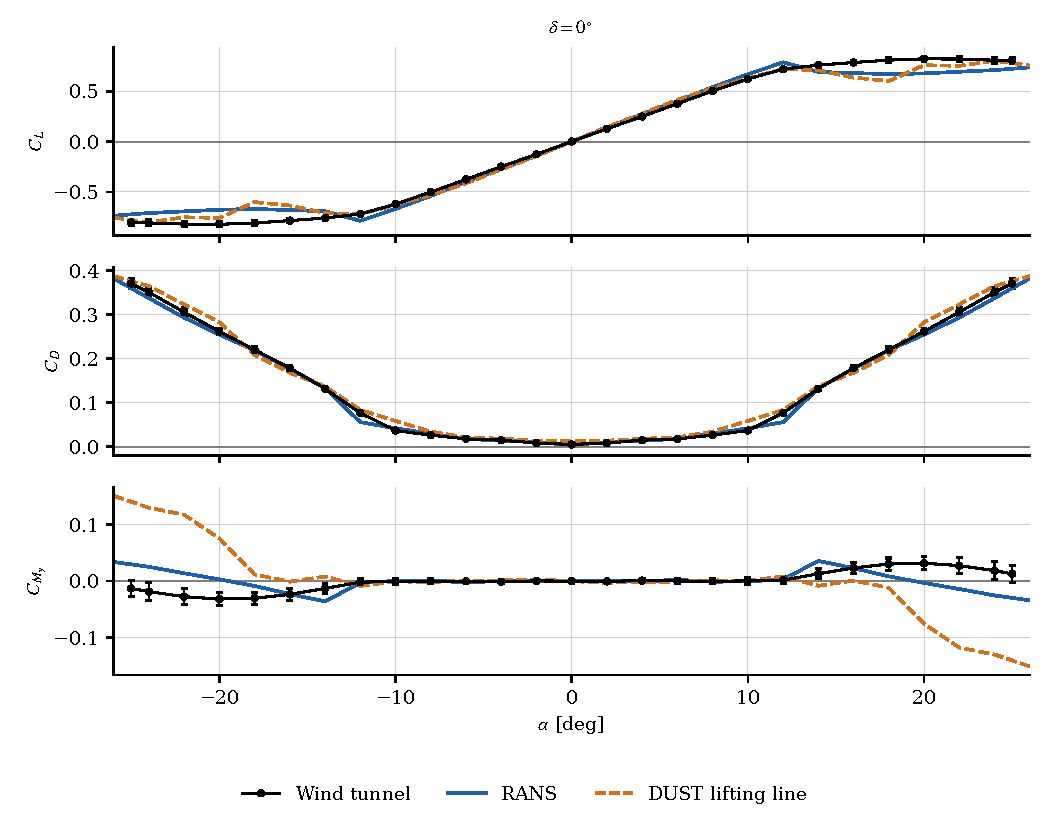
\includegraphics[width=1\linewidth]{Coefficients_baseline.pdf}
    \caption{Wind tunnel, RANS, and DUST lifting-line coefficients for the undeflected tailplane.}
    \label{fig:Coefficients:ExpvsNum:Delta0}
\end{figure}

Figure~\ref{fig:Coefficients:ExpvsNum:Delta0} compares the wind tunnel, RANS, and DUST lifting-line aerodynamic coefficients for the undeflected configuration, $\delta=0^\circ$.
For this symmetric, undeflected configuration, incidence reversal changes the sign of lift and pitching moment while preserving drag.

Starting from the lift coefficient, two main regimes can be identified: an approximately linear attached-flow regime and a nonlinear stall/post-stall regime.
The linear regime extends approximately over $-10^\circ \leq \alpha \leq 10^\circ$, where both numerical approaches are in good agreement with the experimental data.
Beyond this range, the curves become nonlinear, with a more gradual change in the experiment than in the numerical predictions.
The experimental lift slope decreases progressively, consistent with a gradual development of separation. The more localized numerical changes suggest a more abrupt redistribution of surface loading.

Table~\ref{tab:Delta0:AerodynChar} distinguishes the first marked lift-curve slope change from maximum lift.
The incidence of that slope change is denoted by \(\alpha_S\), with \(C_{L,S}=C_L(\alpha_S)\). The subscript \(S\) identifies a marker in the sampled lift curve, rather than a separately measured separation onset.
The peak coefficient \(C_{L,\max}\) and its incidence \(\alpha_{C_{L,\max}}\) are reported independently because lift can continue to increase after the slope change.
The incidence values refer to the sampled points and are limited by their angular spacing.

\begin{table}[htbp]
\centering
\caption{Lift-curve slope-change and maximum-lift characteristics at $\delta=0^\circ$.}
\begin{tabular}{cccc}
\hline
\hline
& Lifting line & RANS & Wind tunnel \\
\hline
$C_{L,S}$ & 0.7210 & 0.7875 & $0.7195\pm0.0160$ \\
$\alpha_{S}$ & $12^\circ$ & $12^\circ$ & $12^\circ$ \\
$C_{L,\max}$ & 0.8022 & 0.7875 & $0.8219\pm0.0226$ \\
$\alpha_{C_{L,\max}}$ & $24^\circ$ & $12^\circ$ & $20^\circ$ \\
\hline
\hline
\end{tabular}
\label{tab:Delta0:AerodynChar}
\end{table}

The slope-change marker occurs at \(\alpha_S=12^\circ\) in all three sampled curves.
At this incidence, the lifting-line prediction is close to the measured \(C_{L,S}\), while RANS overpredicts it.
The experiment subsequently reaches \(C_{L,\max}=0.8219\) at \(20^\circ\), and the lifting-line model reaches a similar maximum at \(24^\circ\).
RANS reaches its maximum at \(12^\circ\), so its slope-change marker and lift peak coincide.
Despite its earlier lift peak, RANS retains substantial lift after stall, consistent with the persistence of suction associated with vortical flow over swept wings~\citep{harper1964sweptstall}.
The lifting-line curve also retains substantial lift but varies less regularly between successive incidences. This behavior may reflect limitations of the sectional-data-based representation when much of the span operates beyond stall.

The drag curves are approximately parabolic over \(\lvert\alpha\rvert\leq10^\circ\), where RANS is closer to the measurements.
The RANS drag curve departs more strongly from this trend near \(12^\circ\), whereas the lifting-line curve changes near \(8^\circ\).
These departures may indicate differences in the predicted development of separation, with a later change in RANS and an earlier change in the lifting-line sectional response. The global curves alone, however, do not locate the separated regions.
At larger absolute incidences, the lifting-line drag has the same irregular variation between sampled conditions as its lift curve.

The pitching-moment coefficient shows larger discrepancies than the lift and drag coefficients.
Table~\ref{tab:Delta0:AC} reports the streamwise coordinate of the aerodynamic center, $x_{AC}$, computed with respect to the leading edge at the root, for each dataset.
The RANS aerodynamic-center coordinate is close to the experimental value, whereas the lifting-line coordinate is approximately $0.07~\mathrm{m}$ farther downstream.
The moment coefficients are evaluated for the undeflected configuration about the aerodynamic center, estimated separately for each dataset.
This choice removes the fitted linear moment slope, making the remaining nonlinear variation easier to compare.
The same axis is retained at nonzero deflections. Outside the linear range, the numerical moment curves depart from the experimental trend.

\begin{table}[htbp]
    \centering
    \caption{Streamwise aerodynamic-center coordinates from the root leading edge for the undeflected tailplane.}
    \begin{tabular}{cccc}
         \hline
         \hline
         & Lifting-line & 3D RANS & Wind Tunnel \\
         \hline
         $x_{AC}$ & $0.7119~\mathrm{m}$ & $0.6420~\mathrm{m}$ & $(0.6426\pm0.0011)~\mathrm{m}$ \\
         \hline
         \hline
    \end{tabular}
    \label{tab:Delta0:AC}
\end{table}

The experimental interval in Table~\ref{tab:Delta0:AC} is obtained by propagating the 95\% slope-fit intervals through the aerodynamic-center estimate, neglecting covariance between the force and moment slopes. It represents fit uncertainty rather than a complete uncertainty bound on the experimental reference position.

Pitching moment depends on the spatial distribution of the aerodynamic forces as well as their resultant.
The continuous experimental moment variation is consistent with a gradual redistribution of suction associated with the separated vortical flow that may also sustain post-stall lift. In particular, a spanwise displacement of the suction region on the swept planform would change its streamwise moment arm relative to the aerodynamic-center axis.
The smoother experimental moment curve and the sharper numerical changes therefore suggest different progressions of this loading redistribution, even where integrated lift levels remain similar. The global coefficients alone do not determine the trajectory of the separated structure.

To examine how the separated-flow pattern sustains lift and redistributes pitching moment, Fig.~\ref{fig:FlowTopology:RefDelta0} compares RANS suction-side loading distributions and skin-friction lines before and after the computed lift drop.
The first row is colored by the local contribution to the lift coefficient per unit surface area, whereas the second row is colored by the local contribution to the pitching-moment coefficient per unit surface area.
In both rows, the black curves denote skin-friction lines, and the white arrows indicate their direction. The green line denotes the aerodynamic-center axis.

\begin{figure}[h!]
\centering
\begin{tabular}{>{\centering\arraybackslash}m{1.4cm}>{\centering\arraybackslash}m{4cm}>{\centering\arraybackslash}m{4cm}>{\centering\arraybackslash}m{4cm}>{\centering\arraybackslash}m{1cm}}
\hline
\hline
&
$\boldsymbol{\alpha} \mathbf{ = 12^\circ}$
&
$\boldsymbol{\alpha} \mathbf{ = 14^\circ}$
&
$\boldsymbol{\alpha} \mathbf{ = 20^\circ}$
&
\\
\hline

\makecell[c]{\textbf{Local}\\ $\mathbf{C_{L}}$}
&
\MaskedImage[width=0.28\textwidth]{RefPlan_AoA_12_Delta_0_UpperSurface_CL.png}{%
    \maskrecttl{0.0}{0.0}{0.3}{0.63}
    \maskrecttl{0.7}{0.72}{0.26}{0.3}
}
&
\MaskedImage[width=0.28\textwidth]{RefPlan_AoA_14_Delta_0_UpperSurface_CL.png}{%
    \maskrecttl{0.0}{0.0}{0.3}{0.63}
    \maskrecttl{0.7}{0.72}{0.26}{0.3}
}

&
\MaskedImage[width=0.28\textwidth]{RefPlan_AoA_20_Delta_0_UpperSurface_CL.png}{%
    \maskrecttl{0.0}{0.0}{0.3}{0.63}
    \maskrecttl{0.7}{0.72}{0.26}{0.3}
}

&
\multirow[c]{1}{*}[1.7cm]{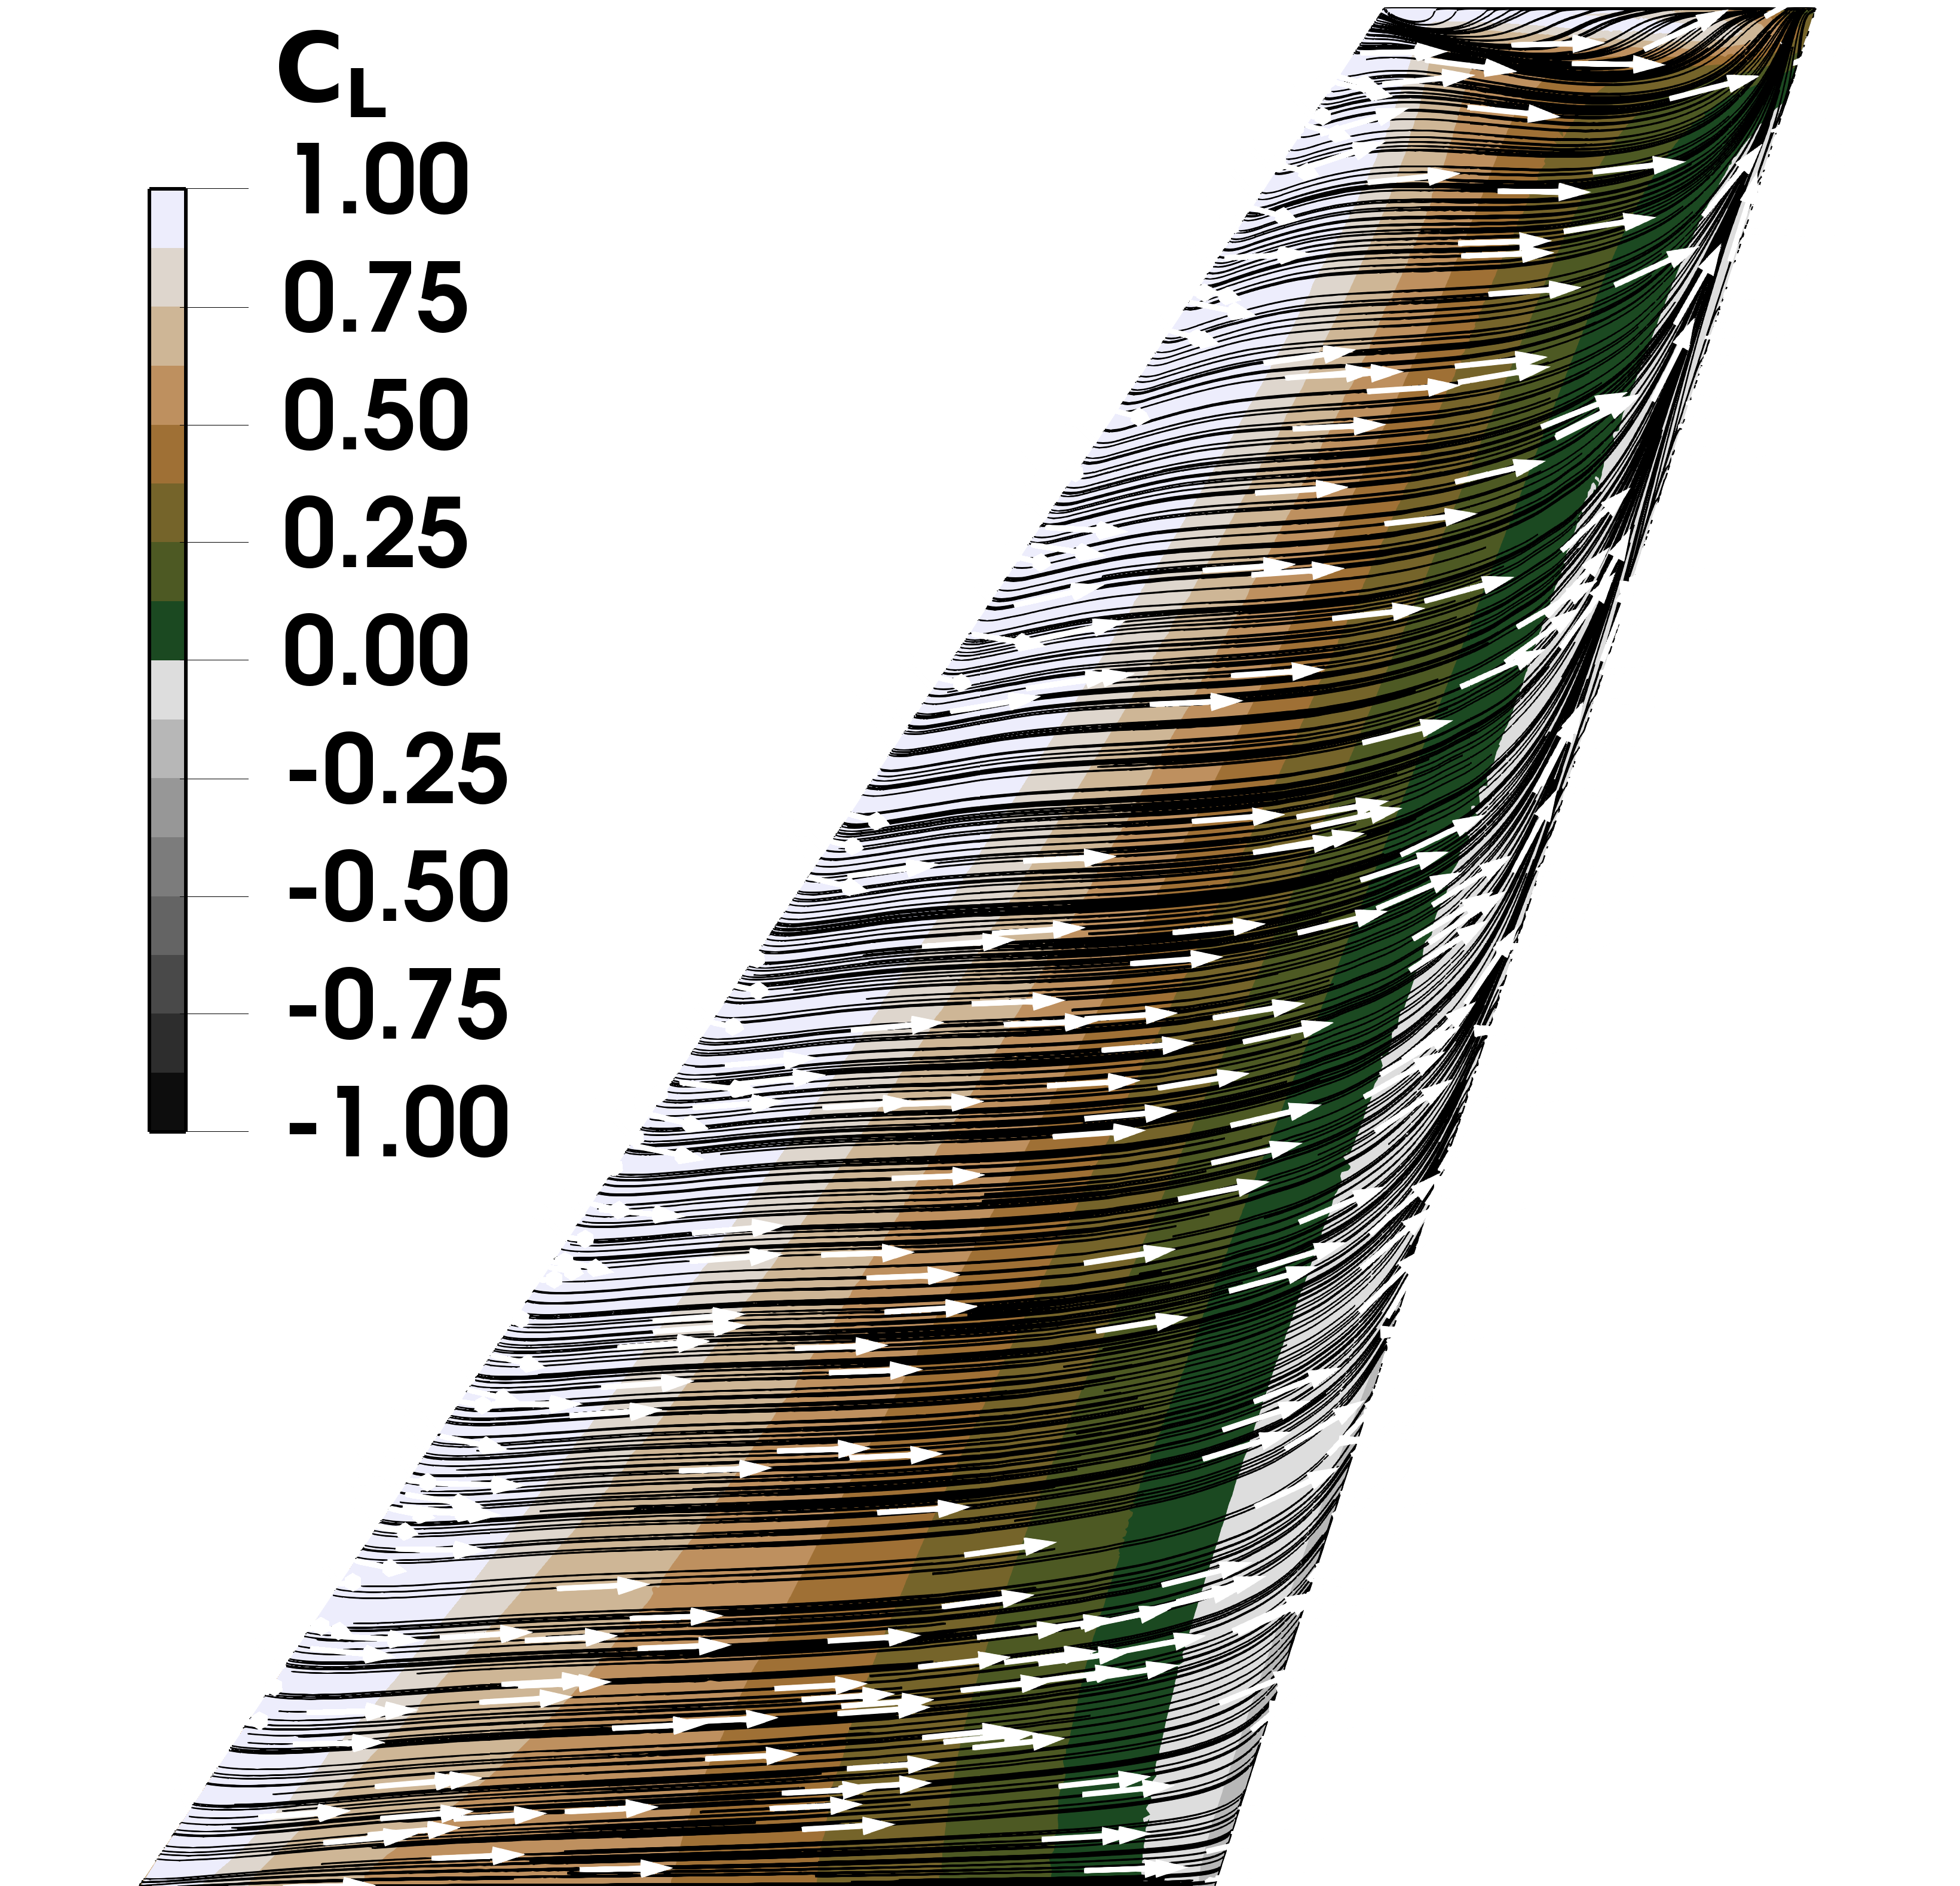
\includegraphics[width=1.2
\linewidth, height=3.6\linewidth, clip, trim={8cm 40cm 84cm 0cm}]{RefPlan_AoA_12_Delta_0_UpperSurface_CL.png}}
\\

\makecell[c]{\textbf{Local}\\ $\mathbf{C_{M_y}}$}
&
\MaskedImage[width=0.28\textwidth]{RefPlan_AoA_12_Delta_0_UpperSurface_CMy.png}{%
    \maskrecttl{0.0}{0.0}{0.3}{0.63}
    \maskrecttl{0.7}{0.72}{0.26}{0.3}
}

&
\MaskedImage[width=0.28\textwidth]{RefPlan_AoA_14_Delta_0_UpperSurface_CMy.png}{%
    \maskrecttl{0.0}{0.0}{0.3}{0.63}
    \maskrecttl{0.7}{0.72}{0.26}{0.3}
}

&
\MaskedImage[width=0.28\textwidth]{RefPlan_AoA_20_Delta_0_UpperSurface_CMy.png}{%
    \maskrecttl{0.0}{0.0}{0.3}{0.63}
    \maskrecttl{0.7}{0.72}{0.26}{0.3}
}

&
\multirow[c]{1}{*}[1.7cm]{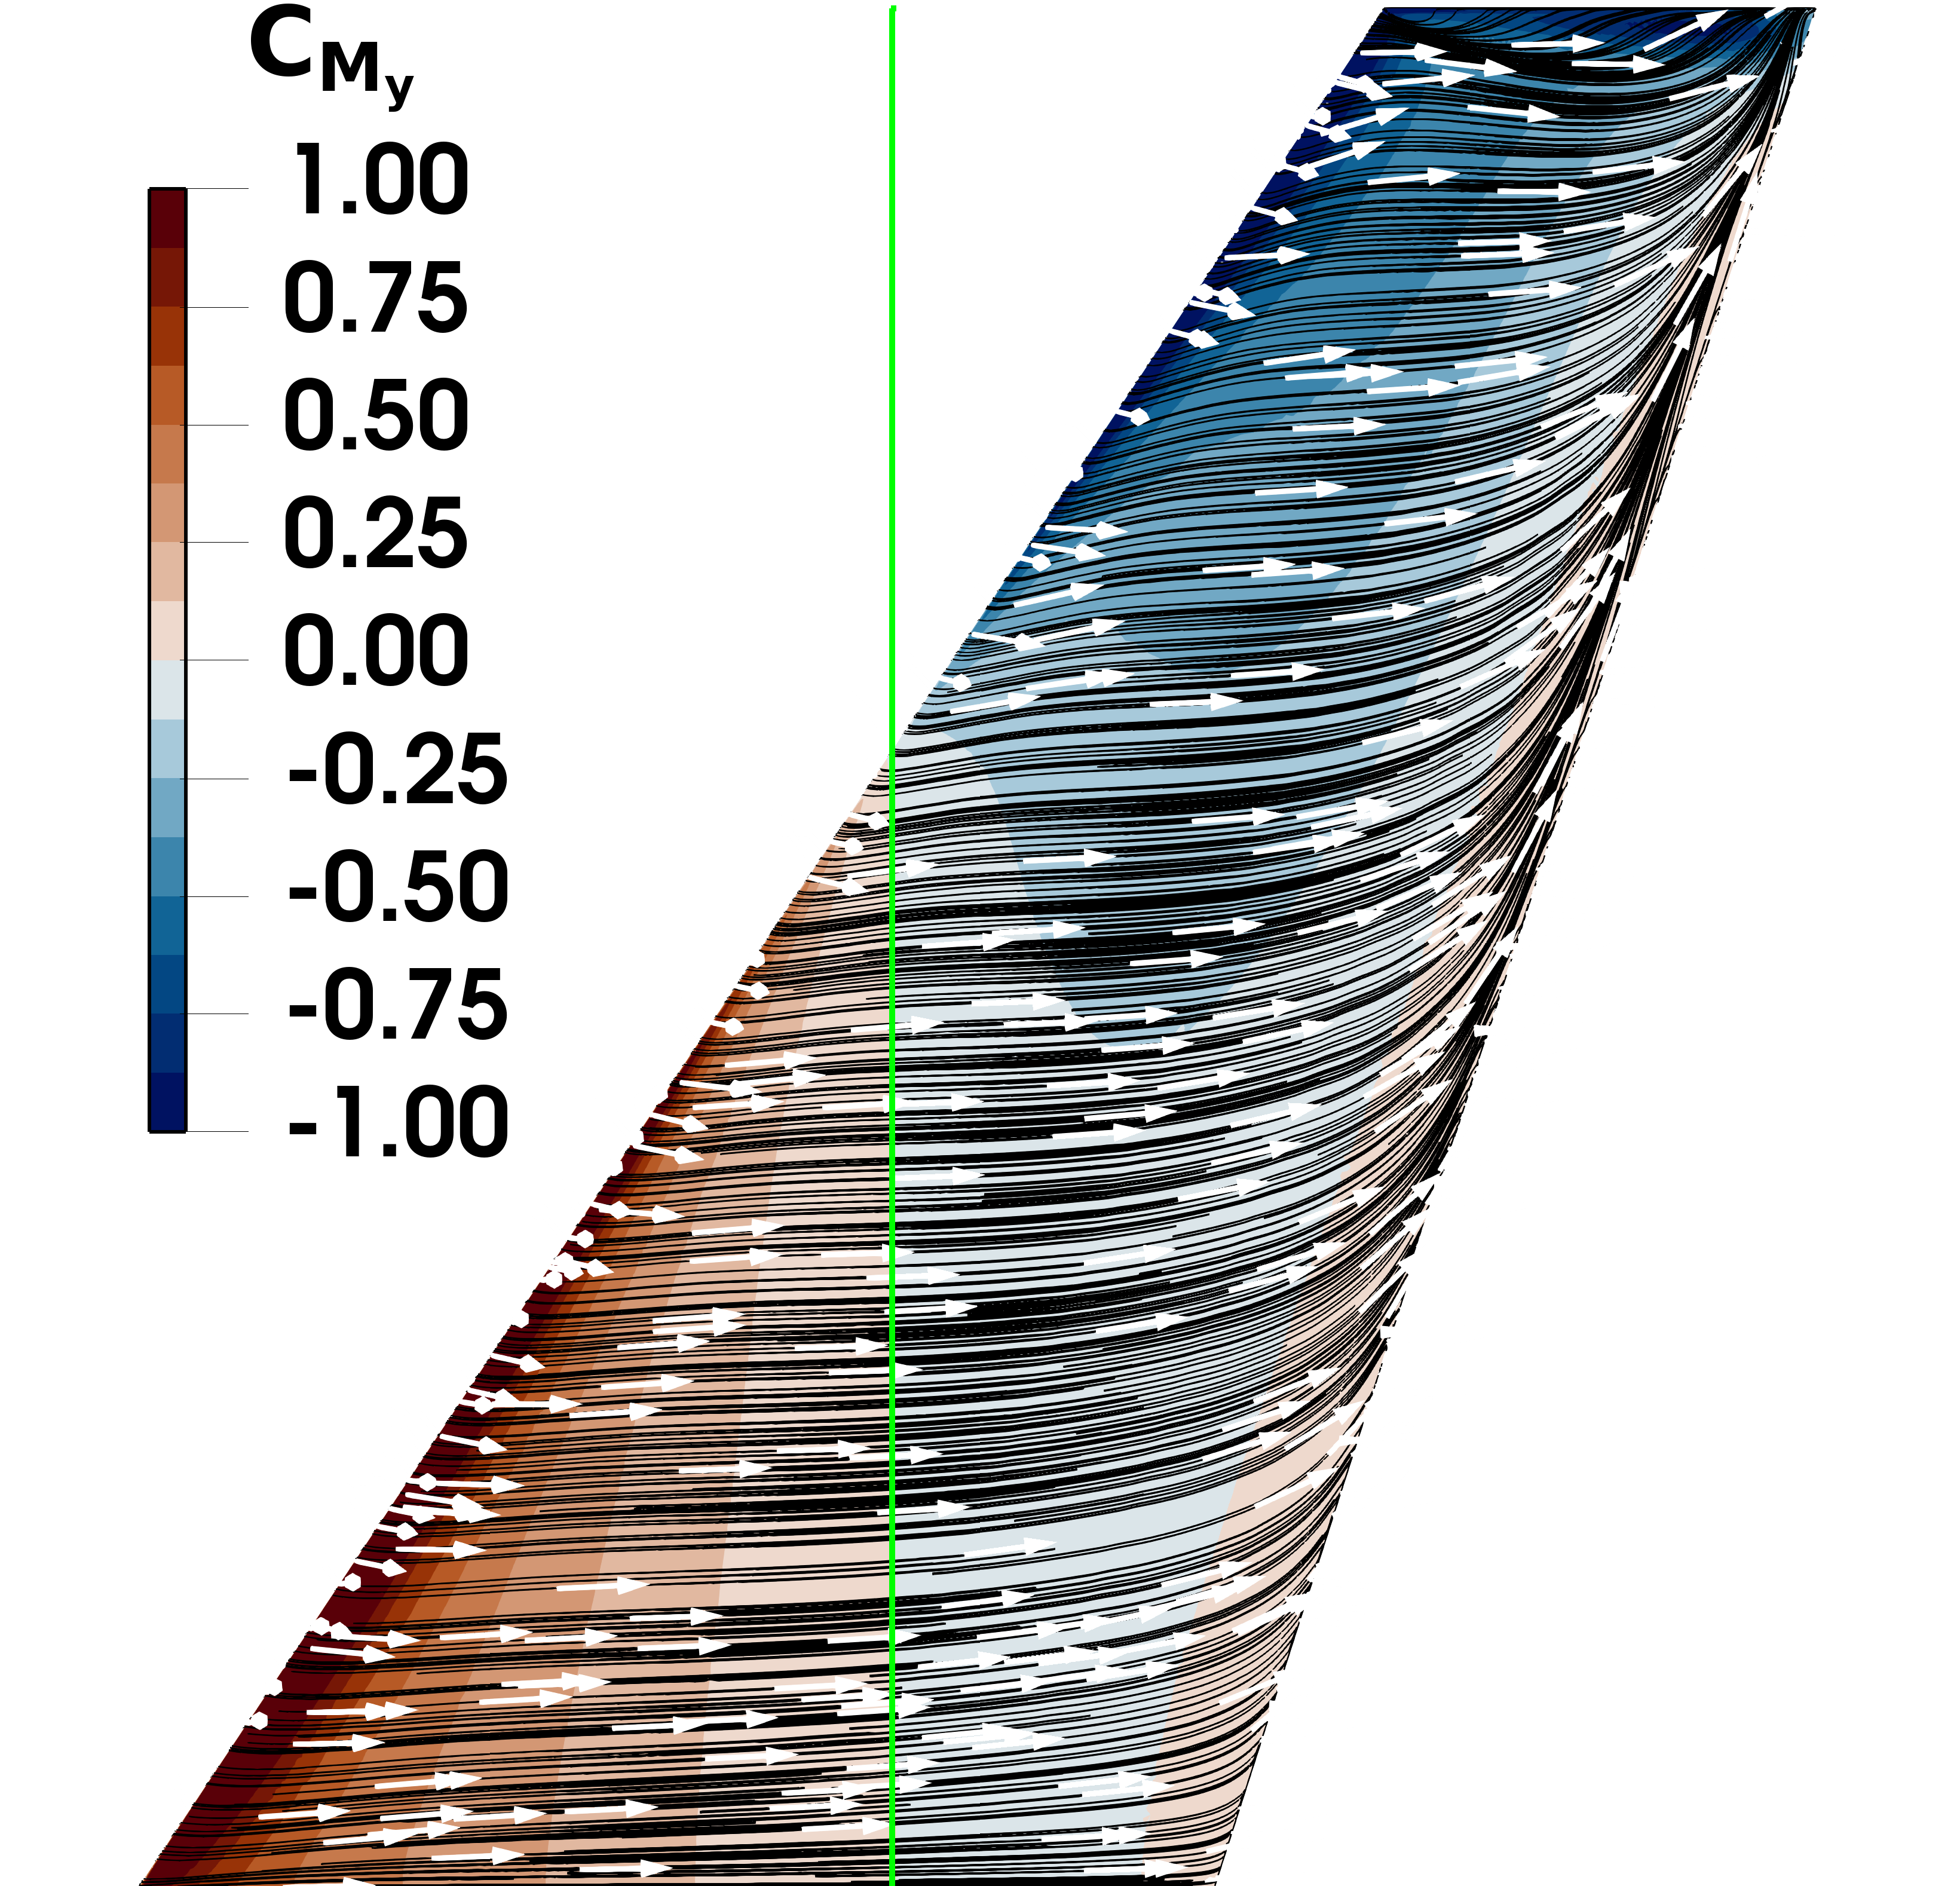
\includegraphics[width=1.2
\linewidth, height=3.6\linewidth, clip, trim={8cm 40cm 84cm 0cm}]{RefPlan_AoA_12_Delta_0_UpperSurface_CMy.png}}

\\
\hline
\hline
\end{tabular}
\caption{RANS suction-side lift- and pitching-moment-coefficient densities with skin-friction lines at \(\delta=0^\circ\).}
\label{fig:FlowTopology:RefDelta0}
\end{figure}

At $\alpha=12^\circ$, the suction-side flow is largely attached, with a spanwise component visible in the skin-friction lines.
At $\alpha=14^\circ$, leading-edge separation develops over a large portion of the upper surface.
This abrupt change in surface topology is consistent with the computed lift drop and drag increase.
At $\alpha=20^\circ$, the skin-friction pattern still indicates recirculating flow near the leading edge, accompanied by a region of positive lift contribution. This supports the interpretation that suction associated with the separated vortical flow helps retain lift after stall.
Its position relative to the aerodynamic-center axis, shown by the green line in the second row, changes only moderately as the incidence increases.
The local moment distribution contains positive contributions in this region and negative contributions near the separated tip, which lies farther from the aerodynamic-center axis. The partial cancellation of these contributions provides an interpretation of the small integrated moment despite substantial local loading.

The baseline comparison therefore shows agreement in the approximately linear lift range, with larger differences in pitching moment and in the transition to post-peak conditions. RANS captures a lift-retaining separated-flow state, although the transition is sharper than in the measurements. The lifting-line results suggest that reasonable integrated lift levels beyond stall do not necessarily imply an adequate description of the associated loading distribution.


\subsection{Effect of full-span control-surface deflection}
\label{sec:deflection_results}

Positive trailing-edge deflection increases the section's effective camber and strengthens the adverse pressure gradient over the control surface.
The coefficient comparison in Fig.~\ref{fig:Coefficients:ExpvsNum:Delta0_10_20_34} examines the resulting loading changes and the onset of nonlinear behavior for all five measured settings. The largest measured and numerical settings are \(34^\circ\) and \(35^\circ\), respectively.

\begin{figure}
\centering
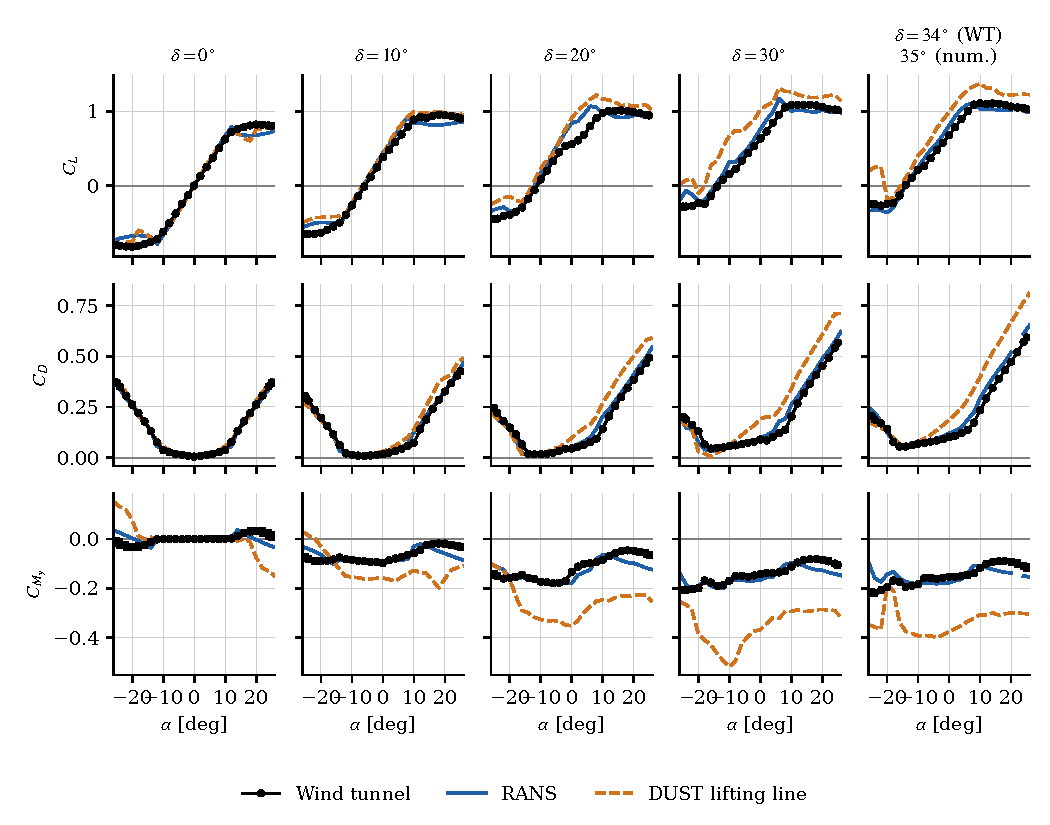
\includegraphics[width=1\linewidth]{Coefficients_selected.pdf}
\caption{Comparison between wind tunnel, RANS, and DUST lifting-line aerodynamic coefficients for all control-surface deflections.}
\label{fig:Coefficients:ExpvsNum:Delta0_10_20_34}
\end{figure}

Figure~\ref{fig:Coefficients:ExpvsNum:Delta0_10_20_34} compares the wind tunnel, RANS, and DUST lifting-line aerodynamic coefficients for $\delta\in\{0^\circ,10^\circ,20^\circ,30^\circ,34^\circ\}$.
At nonzero deflection, the incidence symmetry of the undeflected curves no longer applies, and the positive- and negative-incidence branches differ.

Starting from the lift coefficient, the primary effect of positive control-surface deflection is a vertical shift of the curves.
This trend is consistent with the increase in effective camber produced by a downward deflection of the trailing-edge control surface~\cite{abbott1959theory}.
The measured maximum lift increases with deflection and generally occurs at lower incidence. The numerical methods reproduce the overall increase in maximum lift and reduction in peak-lift incidence, with exceptions at the largest setting: between $30^\circ$ and $35^\circ$, the RANS maximum lift decreases and the peak-lift incidence increases in both numerical models.

At \(\delta=10^\circ\), RANS and lifting-line lift predictions are close up to approximately \(\alpha=8^\circ\).
RANS reaches its maximum at that incidence and then predicts an abrupt lift drop.
The lifting-line curve continues to a broad maximum of approximately \(1.000\) at \(18^\circ\), compared with the measured maximum of approximately \(0.955\) at the same incidence.
For this setting, lifting line reproduces the experimental peak incidence and the smoother post-peak lift evolution more closely than RANS, although it overpredicts the lift level.

As deflection increases, the lifting-line results deviate more substantially from the experimental data.
This behavior is expected because the flow complexity associated with large control-surface deflections is not fully represented by the two-dimensional sectional data used in the C81 tables.
In particular, localized separation over the deflected surface, spanwise load redistribution, and three-dimensional separated-flow effects become increasingly important.
RANS represents the three-dimensional mean-flow redistribution directly, but the predicted coefficient changes still differ from the experiment in the pre-stall nonlinear range.

The lift curves exhibit a localized slope change before main-surface stall, most clearly for \(\delta\geq20^\circ\).
The load decomposition in Fig.~\ref{fig:Coefficients:ExpvsNum:Delta20_34_Division} associates this event with control-surface separation while the fixed surface remains mostly attached, allowing global lift to recover with increasing incidence.

The drag curves shift upward as the control-surface deflection increases.
Moreover, the incidence corresponding to the minimum drag coefficient, $\alpha_{C_{D,\min}}$, moves toward lower values, consistent with the camber increase induced by the deflected trailing edge.
The measured minimum drag changes only moderately up to $\delta=20^\circ$, then increases more strongly at the largest deflections.
This behavior suggests that, beyond a sufficiently large deflection, the control surface is already separated over a broad incidence range, including conditions close to minimum drag.

\begin{figure}
\centering
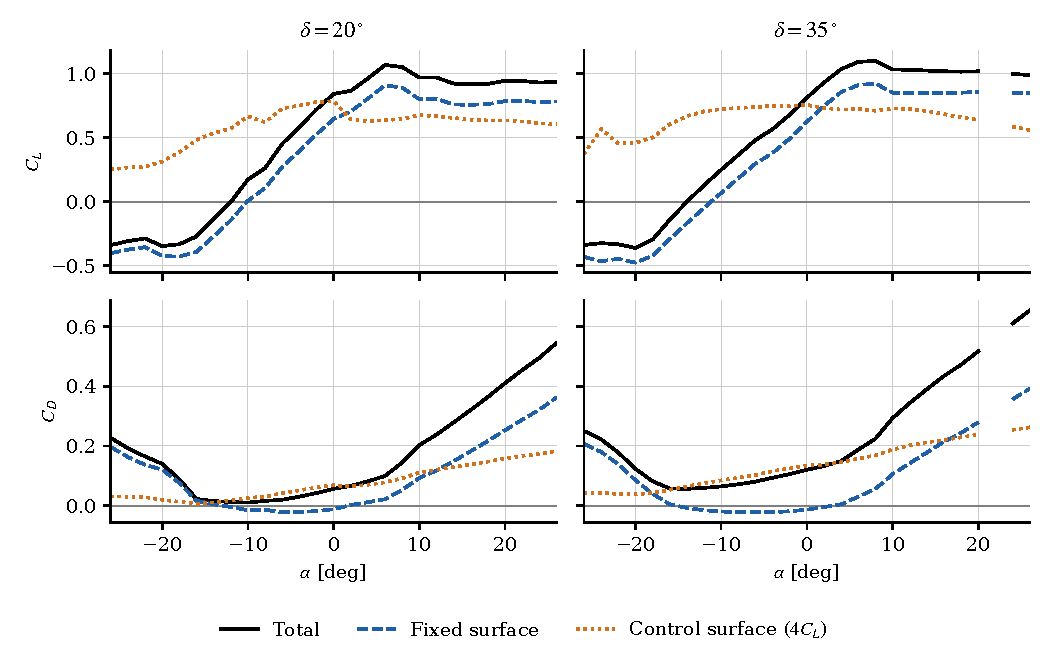
\includegraphics[width=0.9\linewidth]{Load_decomposition.pdf}
\caption{RANS lift and drag contributions from the fixed and control surfaces at \(\delta=20^\circ\) and \(35^\circ\).}
\label{fig:Coefficients:ExpvsNum:Delta20_34_Division}
\end{figure}

Fig.~\ref{fig:Coefficients:ExpvsNum:Delta20_34_Division} supports this interpretation by reporting the RANS load decomposition between the fixed portion of the tailplane and the deflected control surface for $\delta\in\{20^\circ,35^\circ\}$.
The control-surface lift contribution is multiplied by a factor of four to make the local slope variations more visible. The fixed-surface contribution is the sum over the upper and lower main-surface patches; the control contribution also includes its junction and blunt trailing edge. The separate tip patch is included in the total only.
In the attached-flow range of the fixed surface, its contribution to both $C_L$ and $C_D$ is only weakly affected by $\delta$.
Conversely, the control-surface contribution to $C_D$ differs markedly between the two deflections.
For incidences corresponding to the approximately linear part of the global $C_L$--$\alpha$ curve, the deflected surface primarily governs the drag level.

The corresponding control-surface contribution to $C_L$ clarifies the origin of this behavior.
For $\delta=20^\circ$, the lift generated by the control surface increases nearly monotonically up to approximately $\alpha=0^\circ$, where separation begins to affect the local load.
For $\delta=35^\circ$, the control-surface lift contribution is already nearly flat from approximately $\alpha=-10^\circ$, indicating that the deflected surface is separated over a much wider incidence range.
This explains the pronounced upward shift of the drag coefficient between the two deflections.
It also explains the departure of the global $C_D$--$\alpha$ curve from the parabolic trend in the incidence range where the fixed surface is still attached.
In this range, the separated control surface drives the change in drag, while the fixed-surface contribution still retains the parabolic trend typical of attached lifting-surface behavior.

As absolute incidence increases further, the fixed-surface contribution to $C_D$ also grows because separation develops over the main surface.
Since the fixed surface is larger than the control surface, its drag contribution eventually dominates the total drag, especially at large negative incidences.
In this incidence range, the load decomposition indicates that the control surface is no longer the dominant source of the global drag increase.

Figure~\ref{fig:FlowTopology:RefDelta20_34} gives the corresponding local drag distributions. Its columns correspond to \(\alpha=-20^\circ\), \(\alpha=-16^\circ\), and \(\alpha=-12^\circ\).
The upper row reports the contribution per unit surface area to \(C_D\) for \(\delta=20^\circ\), while the lower row reports the corresponding distribution for \(\delta=35^\circ\).
Skin-friction lines are superimposed to indicate the surface-flow topology.

\begin{figure}[h!]
\centering
\begin{tabular}{>{\centering\arraybackslash}m{1.2cm}>{\centering\arraybackslash}m{4cm}>{\centering\arraybackslash}m{4cm}>{\centering\arraybackslash}m{4cm}>{\centering\arraybackslash}m{1cm}}
\hline
\hline
&
$\boldsymbol{\alpha} \mathbf{ = -20^\circ}$
&
$\boldsymbol{\alpha} \mathbf{ = -16^\circ}$
&
$\boldsymbol{\alpha} \mathbf{ = -12^\circ}$
&
\\
\hline

\makecell[c]{\textbf{Local}\\ $\mathbf{C_{D}}$ \\ @ \DeltaCaption{20}}
&
\MaskedImage[width=0.28\textwidth]{RefPlan_AoA_-20_Delta_20_UpperSurface_CD.png}{%
    \maskrecttl{0.0}{0.0}{0.3}{0.63}
    \maskrecttl{0.7}{0.72}{0.26}{0.3}
}
&
\MaskedImage[width=0.28\textwidth]{RefPlan_AoA_-16_Delta_20_UpperSurface_CD.png}{%
    \maskrecttl{0.0}{0.0}{0.3}{0.63}
    \maskrecttl{0.7}{0.72}{0.26}{0.3}
}

&
\MaskedImage[width=0.28\textwidth]{RefPlan_AoA_-12_Delta_20_UpperSurface_CD.png}{%
    \maskrecttl{0.0}{0.0}{0.3}{0.63}
    \maskrecttl{0.7}{0.72}{0.26}{0.3}
}

&
\multirow[c]{1}{*}[1.7cm]{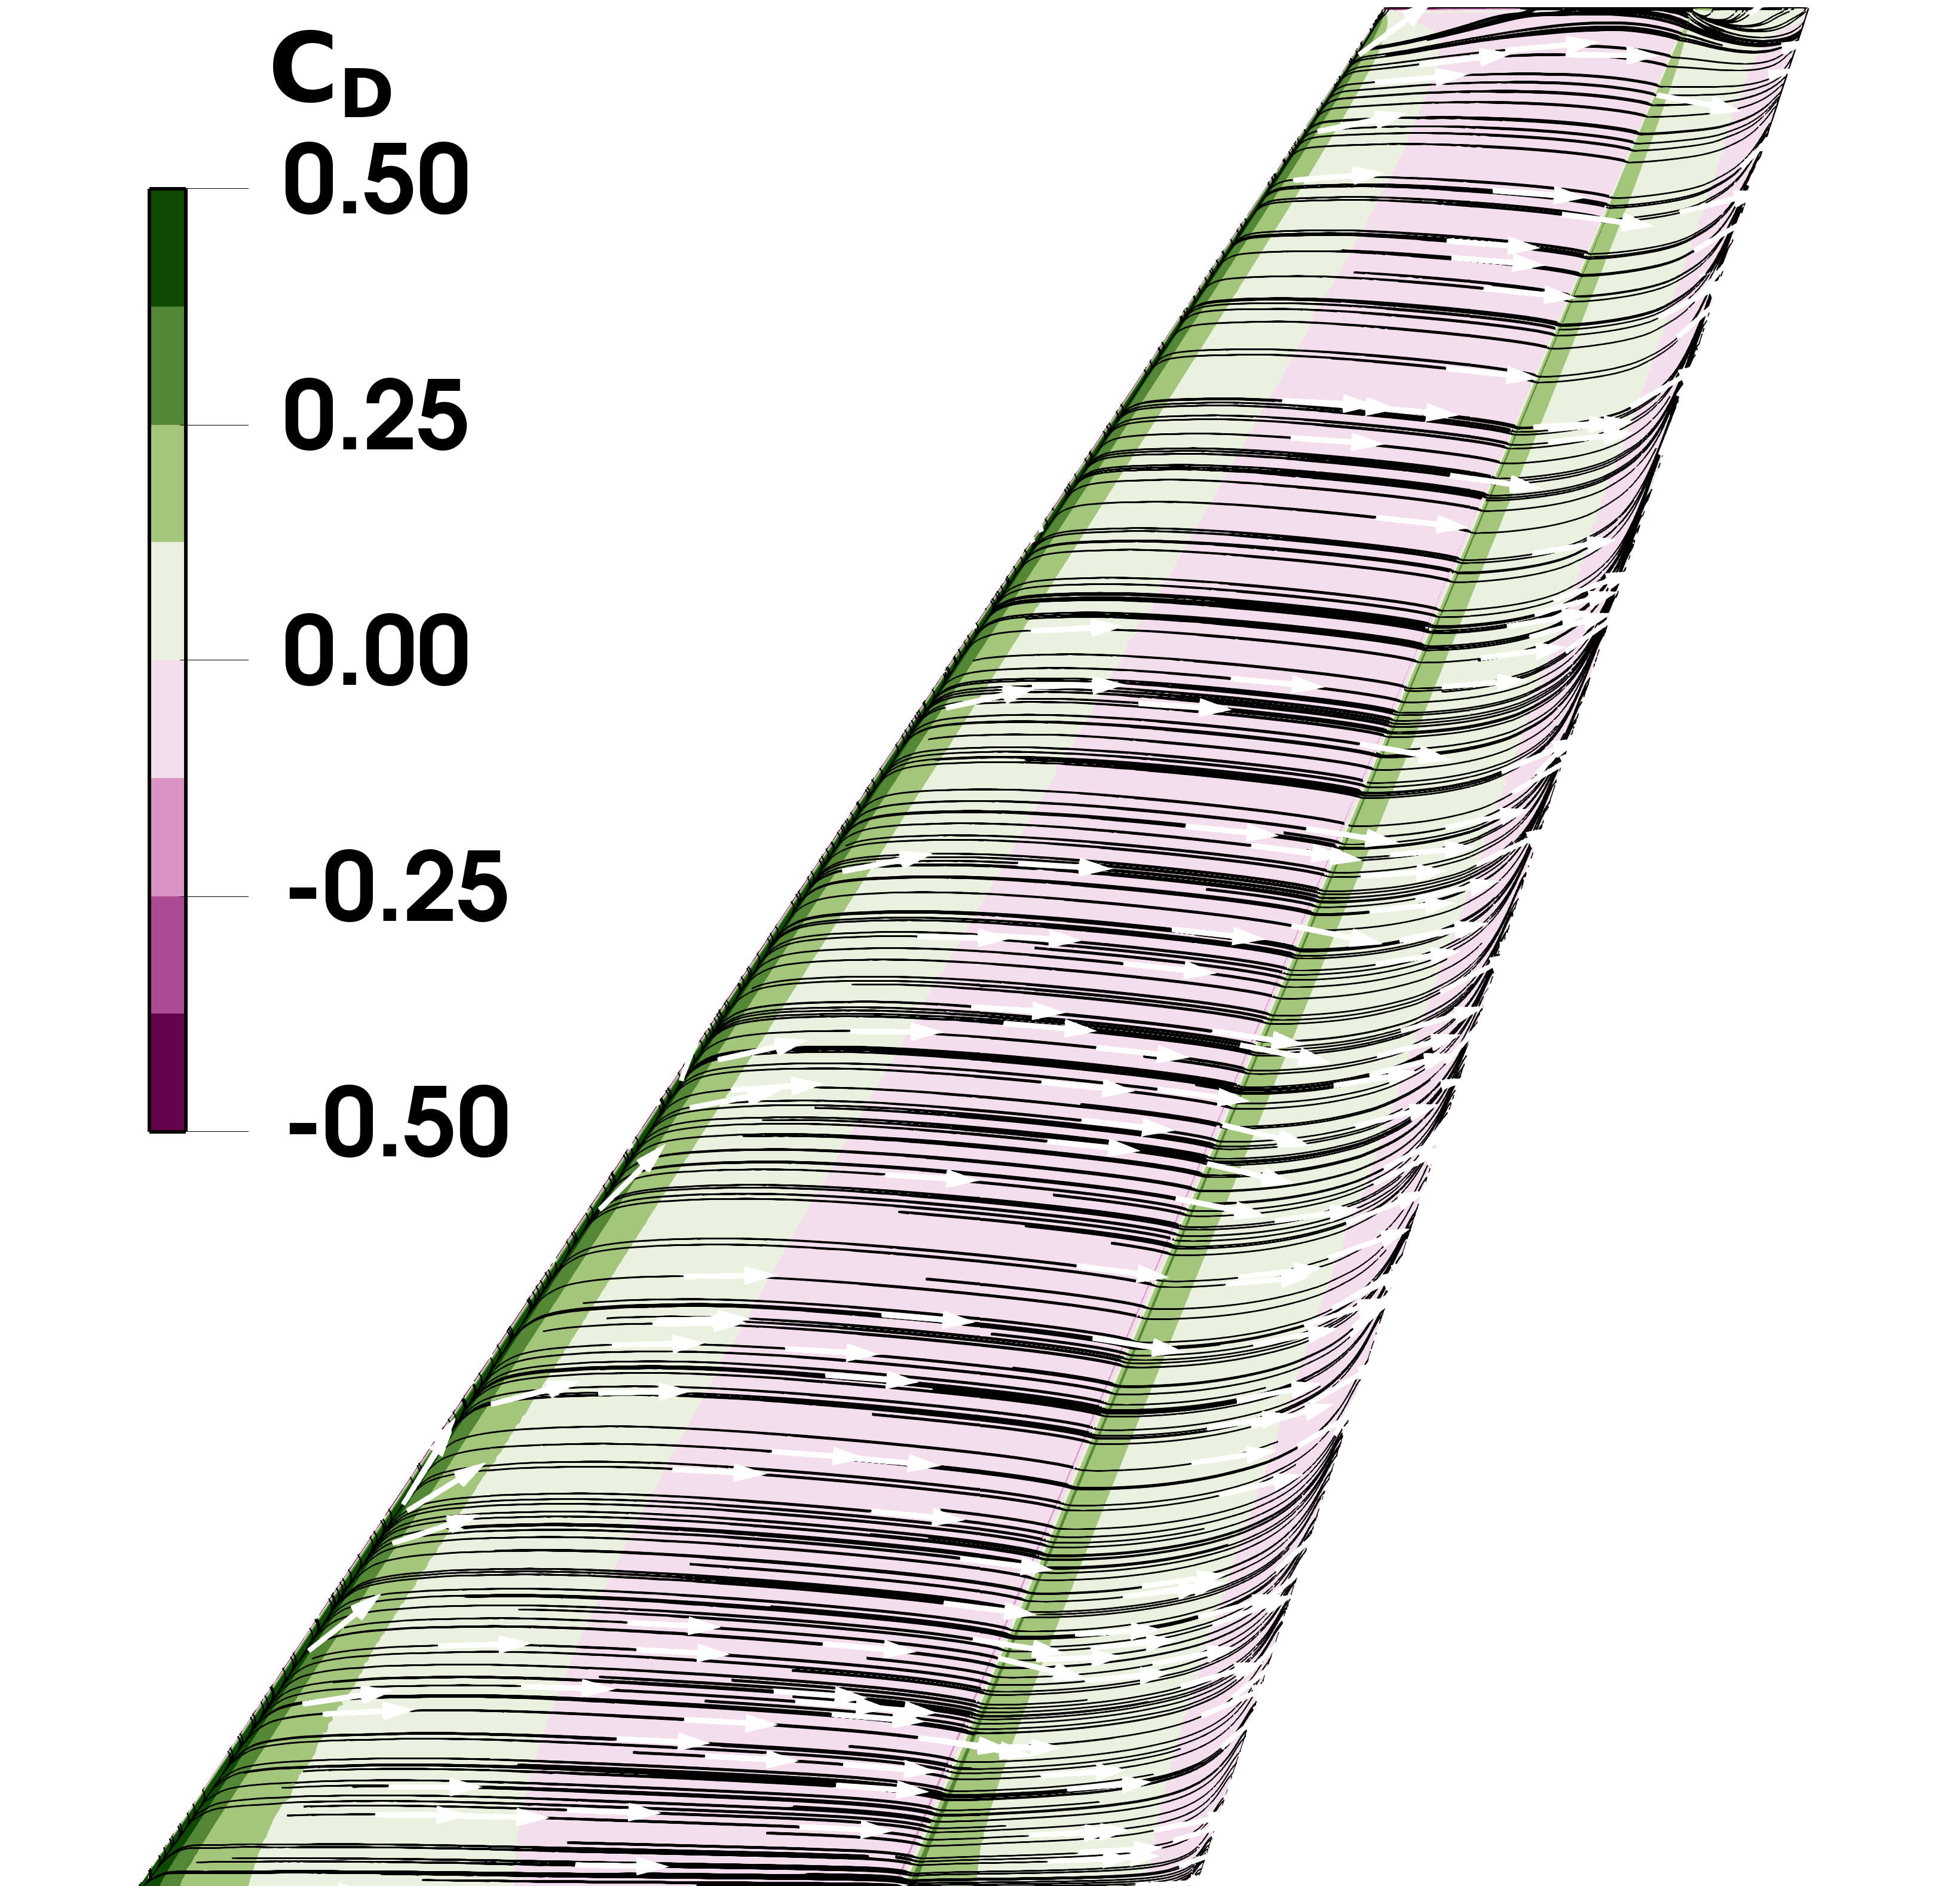
\includegraphics[width=1.2
\linewidth, height=3.6\linewidth, clip, trim={8cm 40cm 84cm 0cm}]{RefPlan_AoA_-12_Delta_20_UpperSurface_CD.png}}
\\

\makecell[c]{\textbf{Local}\\ $\mathbf{C_{D}}$ \\ @ \DeltaCaption{35}}
&
\MaskedImage[width=0.28\textwidth]{RefPlan_AoA_-20_Delta_35_UpperSurface_CD.png}{%
    \maskrecttl{0.0}{0.0}{0.3}{0.63}
    \maskrecttl{0.7}{0.72}{0.26}{0.3}
}

&
\MaskedImage[width=0.28\textwidth]{RefPlan_AoA_-16_Delta_35_UpperSurface_CD.png}{%
    \maskrecttl{0.0}{0.0}{0.3}{0.63}
    \maskrecttl{0.7}{0.72}{0.26}{0.3}
}

&
\MaskedImage[width=0.28\textwidth]{RefPlan_AoA_-12_Delta_35_UpperSurface_CD.png}{%
    \maskrecttl{0.0}{0.0}{0.3}{0.63}
    \maskrecttl{0.7}{0.72}{0.26}{0.3}
}

&
\multirow[c]{1}{*}[1.7cm]{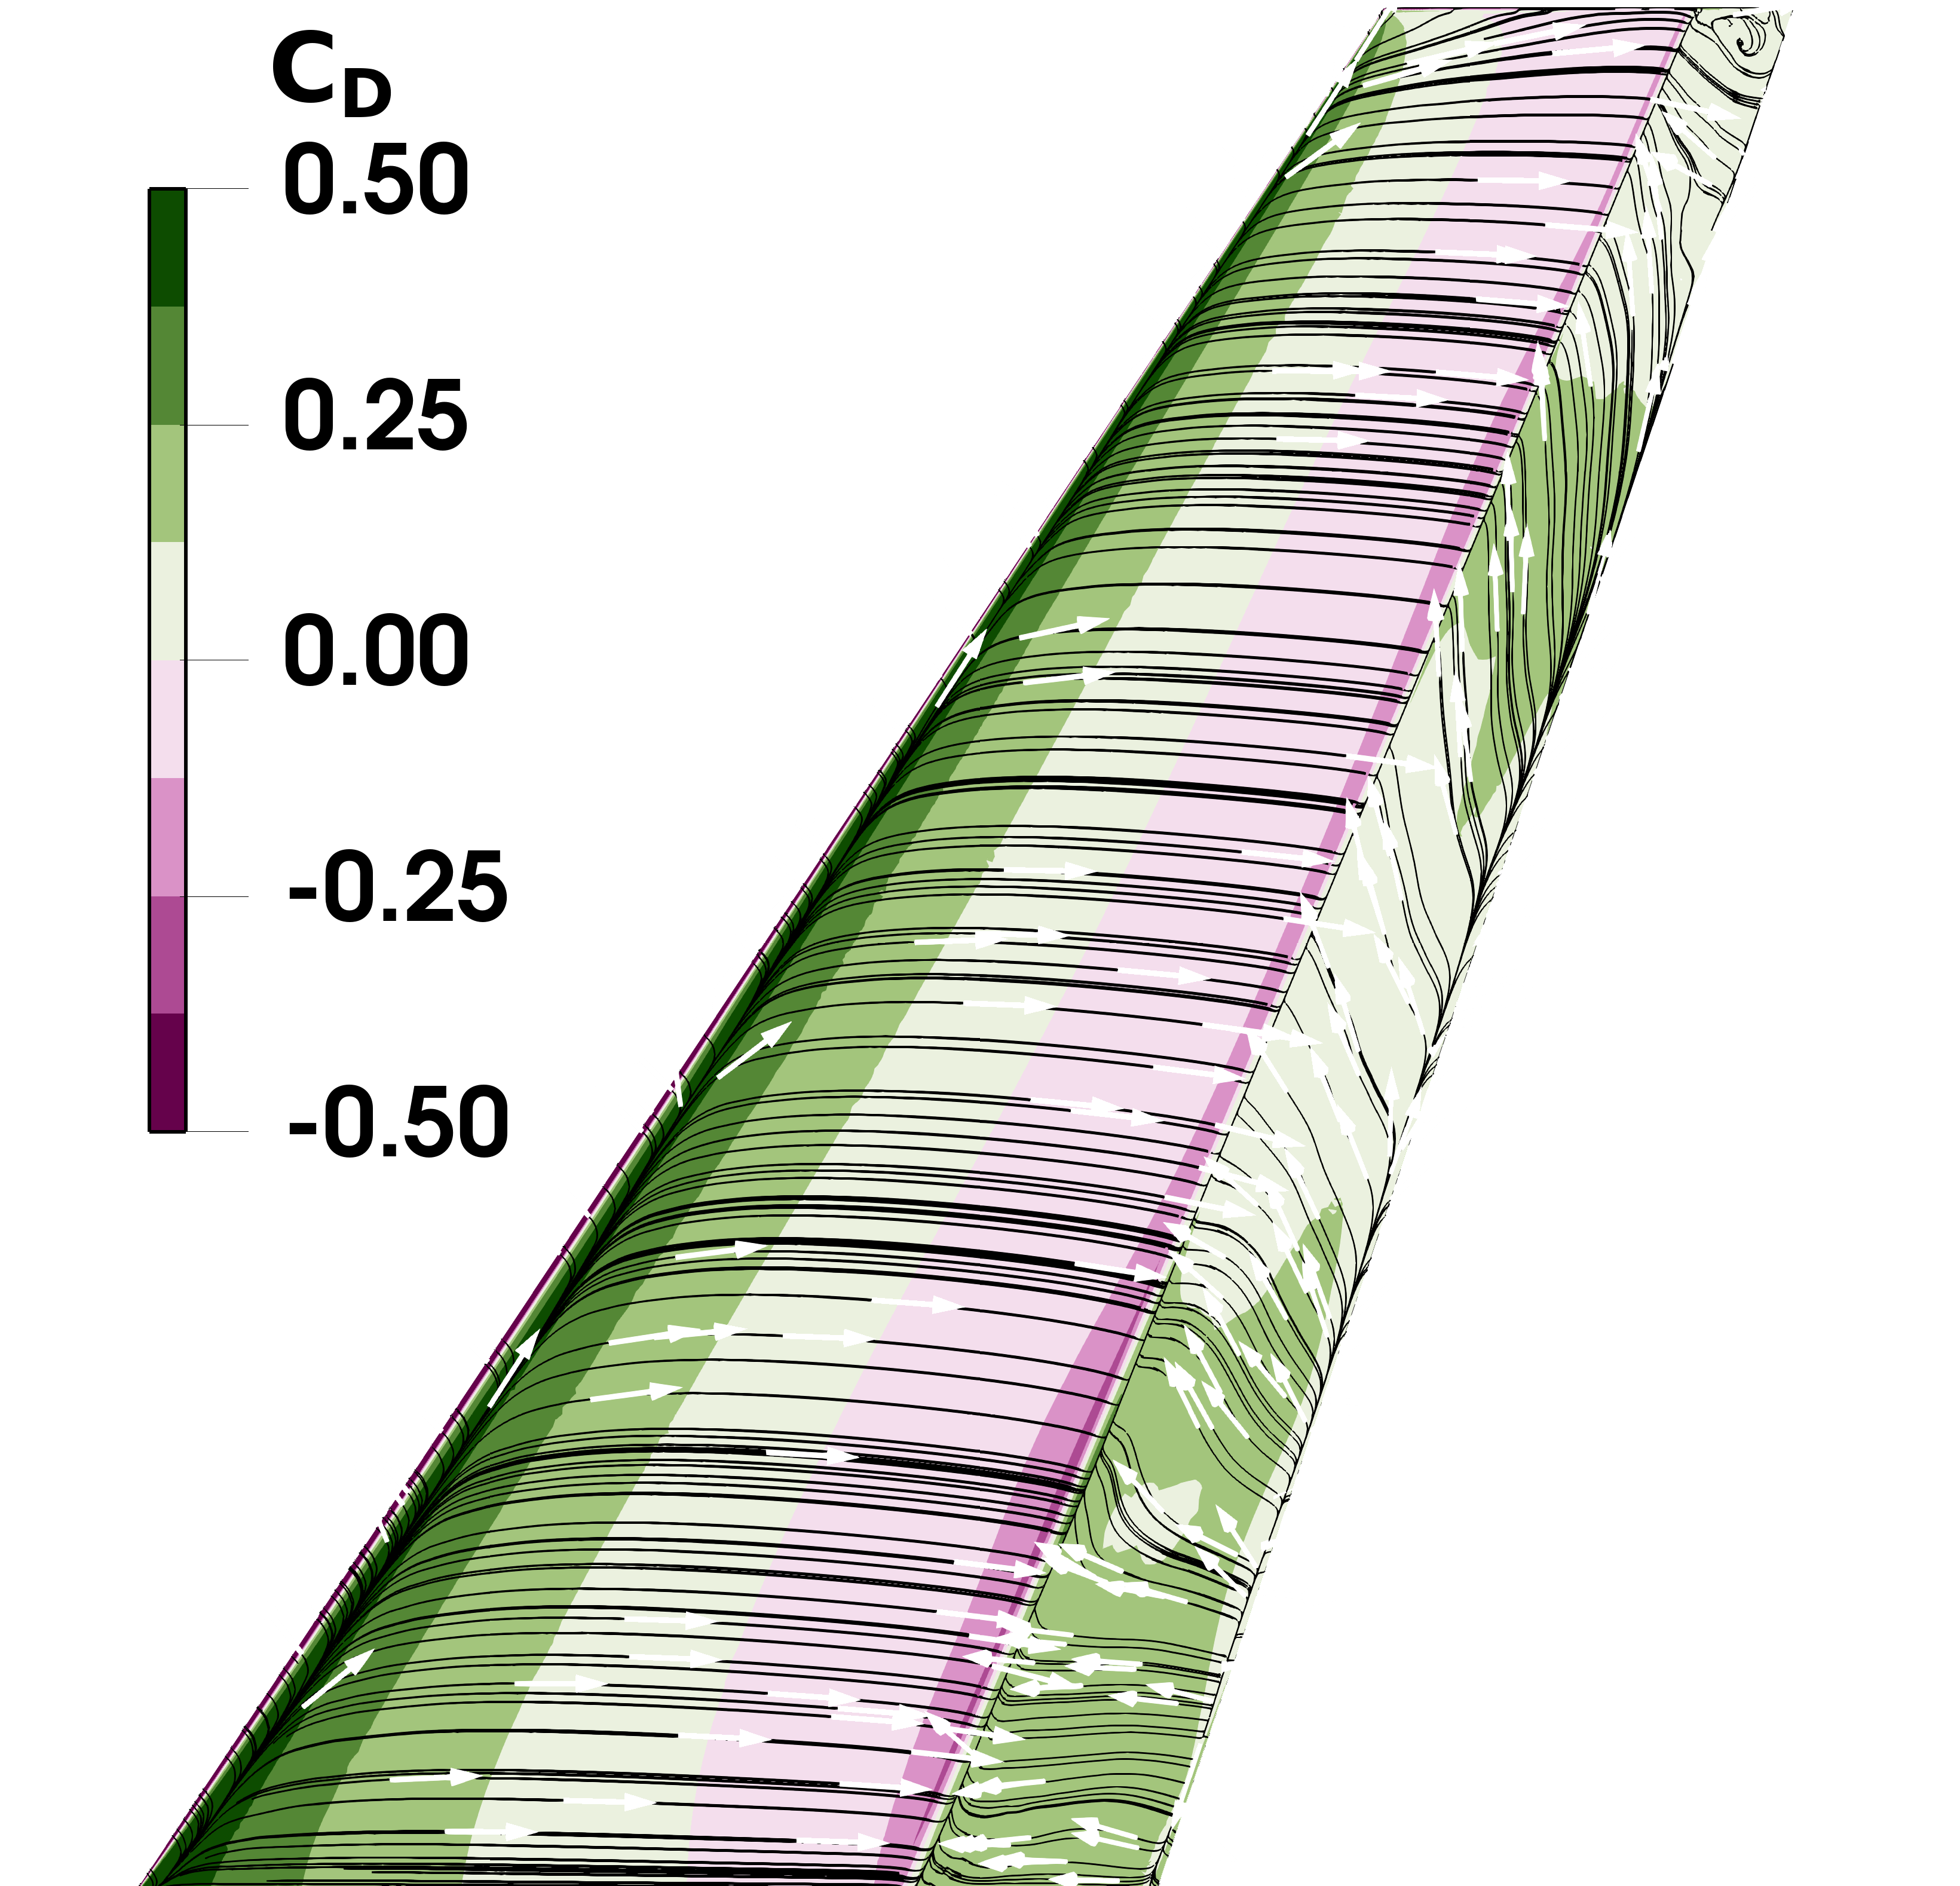
\includegraphics[width=1.2
\linewidth, height=3.6\linewidth, clip, trim={8cm 40cm 84cm 0cm}]{RefPlan_AoA_-20_Delta_35_UpperSurface_CD.png}}

\\
\hline
\hline
\end{tabular}
\caption{RANS surface-flow topology and local drag contributions at \(\delta=20^\circ\) and \(35^\circ\) for negative incidences.}
\label{fig:FlowTopology:RefDelta20_34}
\end{figure}

The skin-friction patterns on the displayed control-surface side are predominantly attached at $\delta=20^\circ$ and separated at $\delta=35^\circ$.
These fields support the interpretation of the integrated curves: the larger deflection produces a separated control-surface state over a wider range of incidence.

The local $C_D$ contribution further clarifies the origin of the drag difference between the two deflections.
For $\delta=35^\circ$, the entire control surface contributes positively to drag.
The fixed surface, by contrast, shows regions of both positive and negative local drag contributions, primarily from the combined effects of the pressure distribution and local surface orientation.
As the angle of attack increases from $\alpha=-20^\circ$ to $\alpha=-12^\circ$, the region of negative local drag contribution expands toward the leading edge.
This increases its influence on the integrated fixed-surface contribution, consistent with the trend reported in Fig.~\ref{fig:Coefficients:ExpvsNum:Delta20_34_Division}.

For $\delta=20^\circ$, the distribution at $\alpha=-20^\circ$ is similar to that obtained for $\delta=35^\circ$ in terms of the fixed-surface contribution.
The integrated RANS lift and drag levels are also close at this incidence.
As incidence increases, the fixed-surface distributions remain broadly similar between the two deflections, whereas the control-surface contribution becomes markedly different.
Since the flow over the control surface remains attached for $\delta=20^\circ$, the aft pressure distribution includes a negative local drag contribution near the trailing edge.
This contribution partly counterbalances the positive drag generated over the rest of the deflected surface, reducing integrated control-surface drag and, therefore, the total drag coefficient.



The pitching-moment curves in Fig.~\ref{fig:Coefficients:ExpvsNum:Delta0_10_20_34} change in both level and slope with control deflection.
Because the reference axis is fitted to the undeflected case, the near-constant linear-range moment at \(\delta=0^\circ\) is a consequence of that choice; it is not imposed on the deflected cases.
At \(\delta=20^\circ\), the change in moment slope near \(\alpha=0^\circ\) occurs alongside the control-surface load change identified in the RANS decomposition.
The experimental curves show a smoother change than the numerical predictions.

The numerical approaches differ substantially in their ability to reproduce the pitching-moment behavior.
For nonzero deflections, the larger lifting-line moment discrepancy shows that agreement in integrated lift does not ensure agreement in the moment of the load distribution.
This limitation is particularly important for $C_{M_y}$ because the moment coefficient depends directly on the load position relative to the aerodynamic center.
The RANS simulations more closely represent the wind tunnel curve shapes, including the rise of $C_{M_y}$ around $\alpha=0^\circ$.
However, the RANS results replace the smoother post-stall evolution observed experimentally with sharper slope changes, consistent with the more abrupt separation behavior already identified in the lift and drag curves.



\subsection{Lift and pitching-moment control effectiveness}
\label{sec:effectiveness_results}


Control effectiveness quantifies the incremental lift and pitching moment produced by a change in deflection at fixed incidence. Its variation with incidence identifies where a constant control derivative is inadequate.

In this study, the interval control effectiveness is the finite-difference approximation of the control derivative at fixed incidence. For \(C_Q\), with \(Q\in\{L,M_y\}\), it is computed as
\begin{equation}
C_{Q,\delta}^{[\delta_i,\delta_j]}(\alpha)
=
\frac{
C_Q(\alpha,\delta_j)-C_Q(\alpha,\delta_i)
}{
\delta_j-\delta_i
},
\label{eq:control_effectiveness_interval}
\end{equation}
where \(\delta\) is expressed in radians. Experimental pointwise uncertainties are obtained by dividing the root-sum-square of the two coefficient uncertainties by the interval width, neglecting covariance between control settings.
The effectiveness is evaluated over the intervals \([0^\circ,10^\circ]\), \([10^\circ,20^\circ]\), \([20^\circ,30^\circ]\), and \([30^\circ,34^\circ]\).
These finite-interval slopes are reported per radian without smoothing; they need not equal a local derivative when the deflection response is nonlinear.

Each method's pitching moment is referred to its own aerodynamic center.
The last numerical interval is \([30^\circ,35^\circ]\), using its actual \(5^\circ\) width.

\begin{figure}
    \centering
    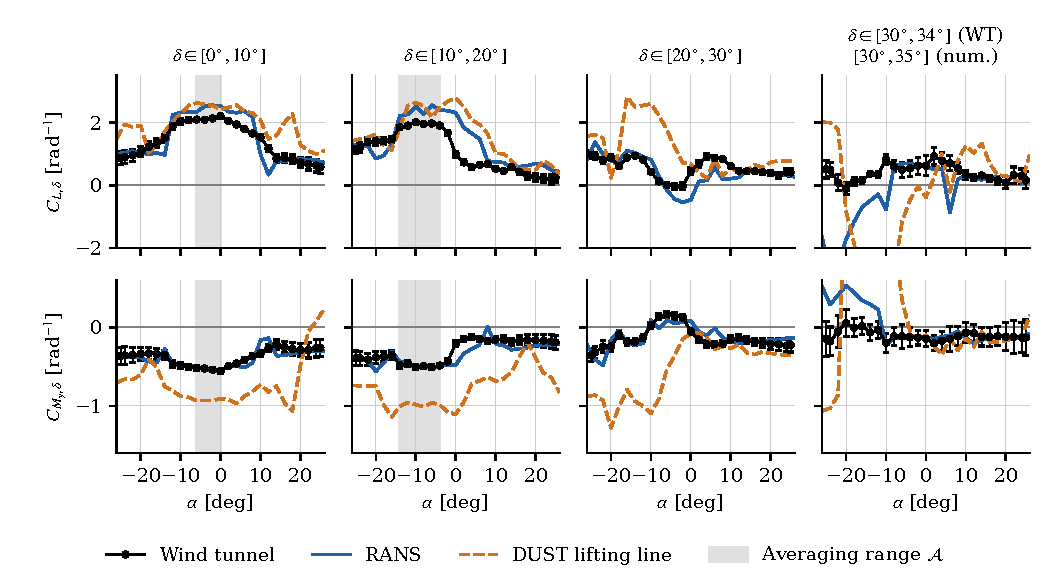
\includegraphics[width=1\linewidth]{ControlEffectiveness_revised.pdf}
    \caption{Lift (top) and pitching-moment (bottom) control effectiveness for successive deflection intervals.}
    \label{fig:AeroCoeffs:control_effectiveness}
\end{figure}

Figure~\ref{fig:AeroCoeffs:control_effectiveness} shows lift effectiveness in the top row and moment effectiveness in the bottom row, with one deflection interval per column.
The positive- and negative-incidence branches differ: the measured lift response is generally greater at negative incidence, while the RANS fields associate the reduction at positive incidence with control-surface separation.

For the low-deflection interval \(\delta\in[0^\circ,10^\circ]\), the \(C_{L,\delta}\) curve exhibits an approximately constant value over the negative and low-incidence range.
This nearly constant response provides the low-deflection reference against which the reductions at larger absolute incidence can be compared.
The wind tunnel results show an initial reduction in control effectiveness at positive incidences, consistent with the change in the \(C_L\)--\(\alpha\) slope visible in Fig.~\ref{fig:Coefficients:ExpvsNum:Delta0_10_20_34}.
Both numerical methods overpredict the measured effectiveness in this regular-response range.
RANS reproduces the initial decrease at small positive incidence, although its effectiveness remains higher than measured and the subsequent reduction is delayed toward larger incidences. The lifting-line response remains nearly flat over this initial decrease.
The measured lift effectiveness decreases progressively towards both ends of the incidence range.
The RANS simulations predict a more abrupt degradation, consistent with the sharper transition between attached and separated states already observed in the global lift curves.
The lifting-line prediction also captures the overall reduction of effectiveness, but its behavior becomes less regular as the flow enters the nonlinear regime.

For the interval \(\delta\in[10^\circ,20^\circ]\), \(C_{L,\delta}\) becomes more strongly dependent on incidence.
On the positive-incidence branch, the wind tunnel curve decreases at low incidence, partially recovers, and then decreases again as the flow approaches stall and post-stall conditions.
This variation is consistent with interaction between control-surface separation and the still-attached fixed-surface loading. The numerical curves reproduce some of the variation but overestimate effectiveness at low positive incidence, suggesting a delayed effect of control-surface separation on the incremental loading.
At higher positive incidences the coefficient differences become smaller as more of the surface enters the separated regime. On the negative-incidence branch, the measured effectiveness remains higher over a wider incidence range, consistent with the deflected surface being less prone to separation under these conditions.

For the interval \(\delta\in[20^\circ,30^\circ]\), the wind tunnel lift effectiveness falls to approximately zero for \(-6^\circ\leq\alpha\leq-2^\circ\), and then recovers to approximately \(0.9\) at \(\alpha=4^\circ\).
In this incidence range, increasing the deflection from \(20^\circ\) to \(30^\circ\) produces little additional lift within the experimental uncertainty.
If the attached-flow response observed at smaller deflections persisted, an additional \(10^\circ\) of deflection would still give a positive lift increment. Instead, the \(20^\circ\) and \(30^\circ\) lift curves nearly coincide in this incidence range. This establishes a loss of incremental lift response. The RANS control-surface unloading in Fig.~\ref{fig:Coefficients:ExpvsNum:Delta20_34_Division} provides a possible separation-related explanation, but the experimental global coefficients alone do not identify which surface regions gain or lose load.
At larger positive incidences, this finite-deflection response approaches a plateau, consistent with the lift-retaining behavior of the separated swept tailplane.
The RANS and measured effectiveness values are closer in the positive-incidence post-peak range.
Around \(\alpha=-2^\circ\), however, RANS predicts a negative lift effectiveness of approximately \(-0.5\), that is, a loss of lift with increasing deflection, which is not observed experimentally.
This discrepancy suggests that RANS predicts the loading change associated with control-surface separation at a different incidence. The lifting-line prediction differs more strongly and varies irregularly with incidence, consistent with limitations of the sectional representation in separated flow.

For the interval \(\delta\in[30^\circ,34^\circ]\), the lift effectiveness is lower over most of the incidence range.
This lower response is consistent with the extensive control-surface separation in the largest-deflection RANS fields.
Because this derivative is computed over a narrow \(4^\circ\) deflection interval, the corresponding curves are more sensitive to local variations and should be interpreted more cautiously than the wider \(10^\circ\) intervals.
The near-zero plateau of the preceding interval is absent, suggesting that the additional deflection does not produce the same change in control-surface state. The larger pointwise uncertainty limits interpretation of smaller variations.

The pitching-moment effectiveness in the bottom row differs more strongly among methods than the lift effectiveness.
The RANS simulations provide the closest overall agreement with the wind tunnel data, whereas the lifting-line results show larger deviations, consistent with the pitching-moment discrepancies discussed in the previous subsection.
At positive incidences, the magnitude of \(C_{M_y,\delta}\) decreases markedly when moving from the low-deflection interval \([0^\circ,10^\circ]\) to the finite-deflection interval \([10^\circ,20^\circ]\).
This reduction indicates a loss of pitching-moment control effectiveness associated with the onset of control-surface separation and with the corresponding redistribution of the incremental aerodynamic load.
At negative incidences, the effectiveness changes less over the same deflection interval, showing that the pitching-moment increments per degree of deflection remain closer to one another on this branch.

For the larger deflection intervals, the wind tunnel curves remain in a lower-effectiveness regime, and further increases in deflection do not produce a comparable additional reduction in \(C_{M_y,\delta}\).
In particular, for the interval \([20^\circ,30^\circ]\), the measured pitching-moment effectiveness becomes positive, approximately \(0.14\)--\(0.17\), for \(-8^\circ\leq\alpha\leq-2^\circ\), in the same range in which the lift effectiveness approaches zero.
The additional deflection therefore produces a nose-up moment increment with little change in net lift, consistent with a redistribution of loading between surface regions rather than a proportional increase in the existing lift distribution. The global coefficients do not locate the compensating load changes. As incidence becomes more negative, the recovery of effectiveness suggests that conditions over the control surface become less prone to separation. The resulting incidence dependence cannot be represented by a single constant control derivative.

For the last interval, \(\delta\in[30^\circ,34^\circ]\), the wind tunnel pitching-moment effectiveness is low and affected by larger uncertainty.
The numerical curves also differ substantially from the measured trend, particularly at negative incidence. Small differences in the predicted control-surface separation state could produce large differences in the incremental loads, particularly where the response changes rapidly. The narrower interval amplifies both experimental uncertainty and differences between the predicted loads at its endpoints.


Table~\ref{tab:control_effectiveness} compares the mean lift and pitching-moment effectiveness for the deflection intervals \([0^\circ,10^\circ]\) and \([10^\circ,20^\circ]\). For each method and interval, the arithmetic mean is taken over the same four incidences, so that changes in the averaging conditions do not affect the comparison.

The selected samples are \(\mathcal{A}=\{-10^\circ,-8^\circ,-6^\circ,-4^\circ\}\), shown by the grey bands in Fig.~\ref{fig:AeroCoeffs:control_effectiveness}.
Over these samples, the measured lift effectiveness lies between \(2.036\) and \(2.088~\mathrm{rad}^{-1}\) for \([0^\circ,10^\circ]\), and between \(1.901\) and \(2.004~\mathrm{rad}^{-1}\) for \([10^\circ,20^\circ]\); every value is within \(3\%\) of its interval mean.
The adjacent samples explain the limits of this range. At \(\alpha=-12^\circ\), the first interval has already fallen to \(1.874~\mathrm{rad}^{-1}\), whereas at \(\alpha=-2^\circ\), the second interval has fallen to \(1.673~\mathrm{rad}^{-1}\).
Including either end would mix the approximately constant response with its incidence-dependent reduction.
The larger deflection intervals are omitted because neither has a comparable plateau over this common range.
The range is selected for the regularity of the measured lift response, rather than from a separate local-flow criterion.

All moments use each method's own undeflected aerodynamic-center axis.
The experimental uncertainty shown is the mean of the pointwise propagated uncertainty intervals; it is not a confidence interval of the mean.

\begin{table}[htbp]
\centering
\caption{Mean control effectiveness over the common incidence range \(-10^\circ\leq\alpha\leq-4^\circ\) (per radian).}
\label{tab:control_effectiveness}
\begin{tabular}{llcc}
\hline\hline
Method & Deflection interval & \(\overline{C}_{L,\delta}\) & \(\overline{C}_{M_y,\delta}\) \\
\hline
Wind tunnel & \([0^\circ,10^\circ]\) & \(2.071\pm0.060\) & \(-0.507\pm0.030\) \\
Wind tunnel & \([10^\circ,20^\circ]\) & \(1.955\pm0.046\) & \(-0.498\pm0.030\) \\
\hline
RANS & \([0^\circ,10^\circ]\) & 2.374 & -0.507 \\
RANS & \([10^\circ,20^\circ]\) & 2.428 & -0.502 \\
\hline
DUST lifting line & \([0^\circ,10^\circ]\) & 2.501 & -0.909 \\
DUST lifting line & \([10^\circ,20^\circ]\) & 2.450 & -0.985 \\
\hline\hline
\end{tabular}
\end{table}

On this common incidence range, the measured mean lift effectiveness decreases by approximately \(6\%\) between the two deflection intervals, while the magnitude of the mean moment effectiveness changes by approximately \(2\%\).
These changes are small compared with the strong reduction near zero incidence: for \([10^\circ,20^\circ]\), measured lift effectiveness falls from approximately \(1.9~\mathrm{rad}^{-1}\) at \(\alpha=-4^\circ\) to \(1.0~\mathrm{rad}^{-1}\) at \(\alpha=0^\circ\), then to \(0.7~\mathrm{rad}^{-1}\) at \(\alpha=2^\circ\).
The mean values therefore provide a reference for comparing methods before that loss; the complete curves remain necessary to describe the control response outside the selected range.

The percentage differences between methods compare the central values in Table~\ref{tab:control_effectiveness}.
RANS overpredicts mean lift effectiveness by approximately \(15\%\) and \(24\%\), respectively, but reproduces mean moment effectiveness within \(1\%\) in both intervals.
DUST overpredicts mean lift effectiveness by approximately \(21\%\) and \(25\%\), while the magnitude of its mean moment effectiveness is approximately \(79\%\) and \(98\%\) too large.
Thus reasonable agreement in lift response does not guarantee comparable agreement in pitching moment.
This difference is not removed by using a common moment axis: transporting the DUST moments with the body-normal force to the experimental aerodynamic-center axis gives mean effectiveness values of approximately \(-1.164\) and \(-1.232~\mathrm{rad}^{-1}\), versus \(-0.507\) and \(-0.498~\mathrm{rad}^{-1}\) experimentally.



\subsection{Main-surface stall and post-stall behavior}
\label{sec:main_stall_results}

The higher-incidence comparison distinguishes separation of the control surface from separation spreading over the fixed main surface.
Figure~\ref{fig:FlowTopology:Delta_0_10_20_34} shows three RANS states for each deflection: maximum lift, a post-peak state after the marked lift drop, and a later post-stall state.
The actual incidences are printed in the panels; the post-peak state is selected to show the developed lift drop and is not always the immediately following computed point.

\begin{figure}[h!]
\centering
\begin{tabular}{>{\centering\arraybackslash}m{1.2cm}>{\centering\arraybackslash}m{4cm}>{\centering\arraybackslash}m{4cm}>{\centering\arraybackslash}m{4cm}>{\centering\arraybackslash}m{1cm}}
\hline
\hline
&
$\boldsymbol{\alpha}_{\mathbf{C_{L,\mathrm{\mathbf{max}}}},\mathrm{\mathbf{RANS}}}$
&
$\boldsymbol{\alpha}_{\mathbf{C}_{\mathbf{L}}^\mathrm{\mathbf{drop}},\mathrm{\mathbf{RANS}}}$
&
$\boldsymbol{\alpha}_{\mathbf{C}_{\mathbf{L,\mathrm{\mathbf{min}}}}^{\mathrm{\mathbf{post}}},\mathrm{\mathbf{RANS}}}$
&
\\
\hline

\makecell[c]{\DeltaCaption{0}}
&
\MaskedImage[width=0.28\textwidth]{RefPlan_AoA_12_Delta_0_UpperSurface_CP.png}{%
    \maskrecttl{0.0}{0.0}{0.3}{0.63}
    \maskrecttl{0.7}{0.72}{0.26}{0.3}
    \node[] at (0.3,0.7) {\AlphaSimple{12}};
}
&
\MaskedImage[width=0.28\textwidth]{RefPlan_AoA_14_Delta_0_UpperSurface_CP.png}{%
    \maskrecttl{0.0}{0.0}{0.3}{0.63}
    \maskrecttl{0.7}{0.72}{0.26}{0.3}
    \node[] at (0.3,0.7) {\AlphaSimple{14}};
}

&
\MaskedImage[width=0.28\textwidth]{RefPlan_AoA_18_Delta_0_UpperSurface_CP.png}{%
    \maskrecttl{0.0}{0.0}{0.3}{0.63}
    \maskrecttl{0.7}{0.72}{0.26}{0.3}
    \node[] at (0.3,0.7) {\AlphaSimple{18}};
}

&
\multirow[c]{1}{*}[1.7cm]{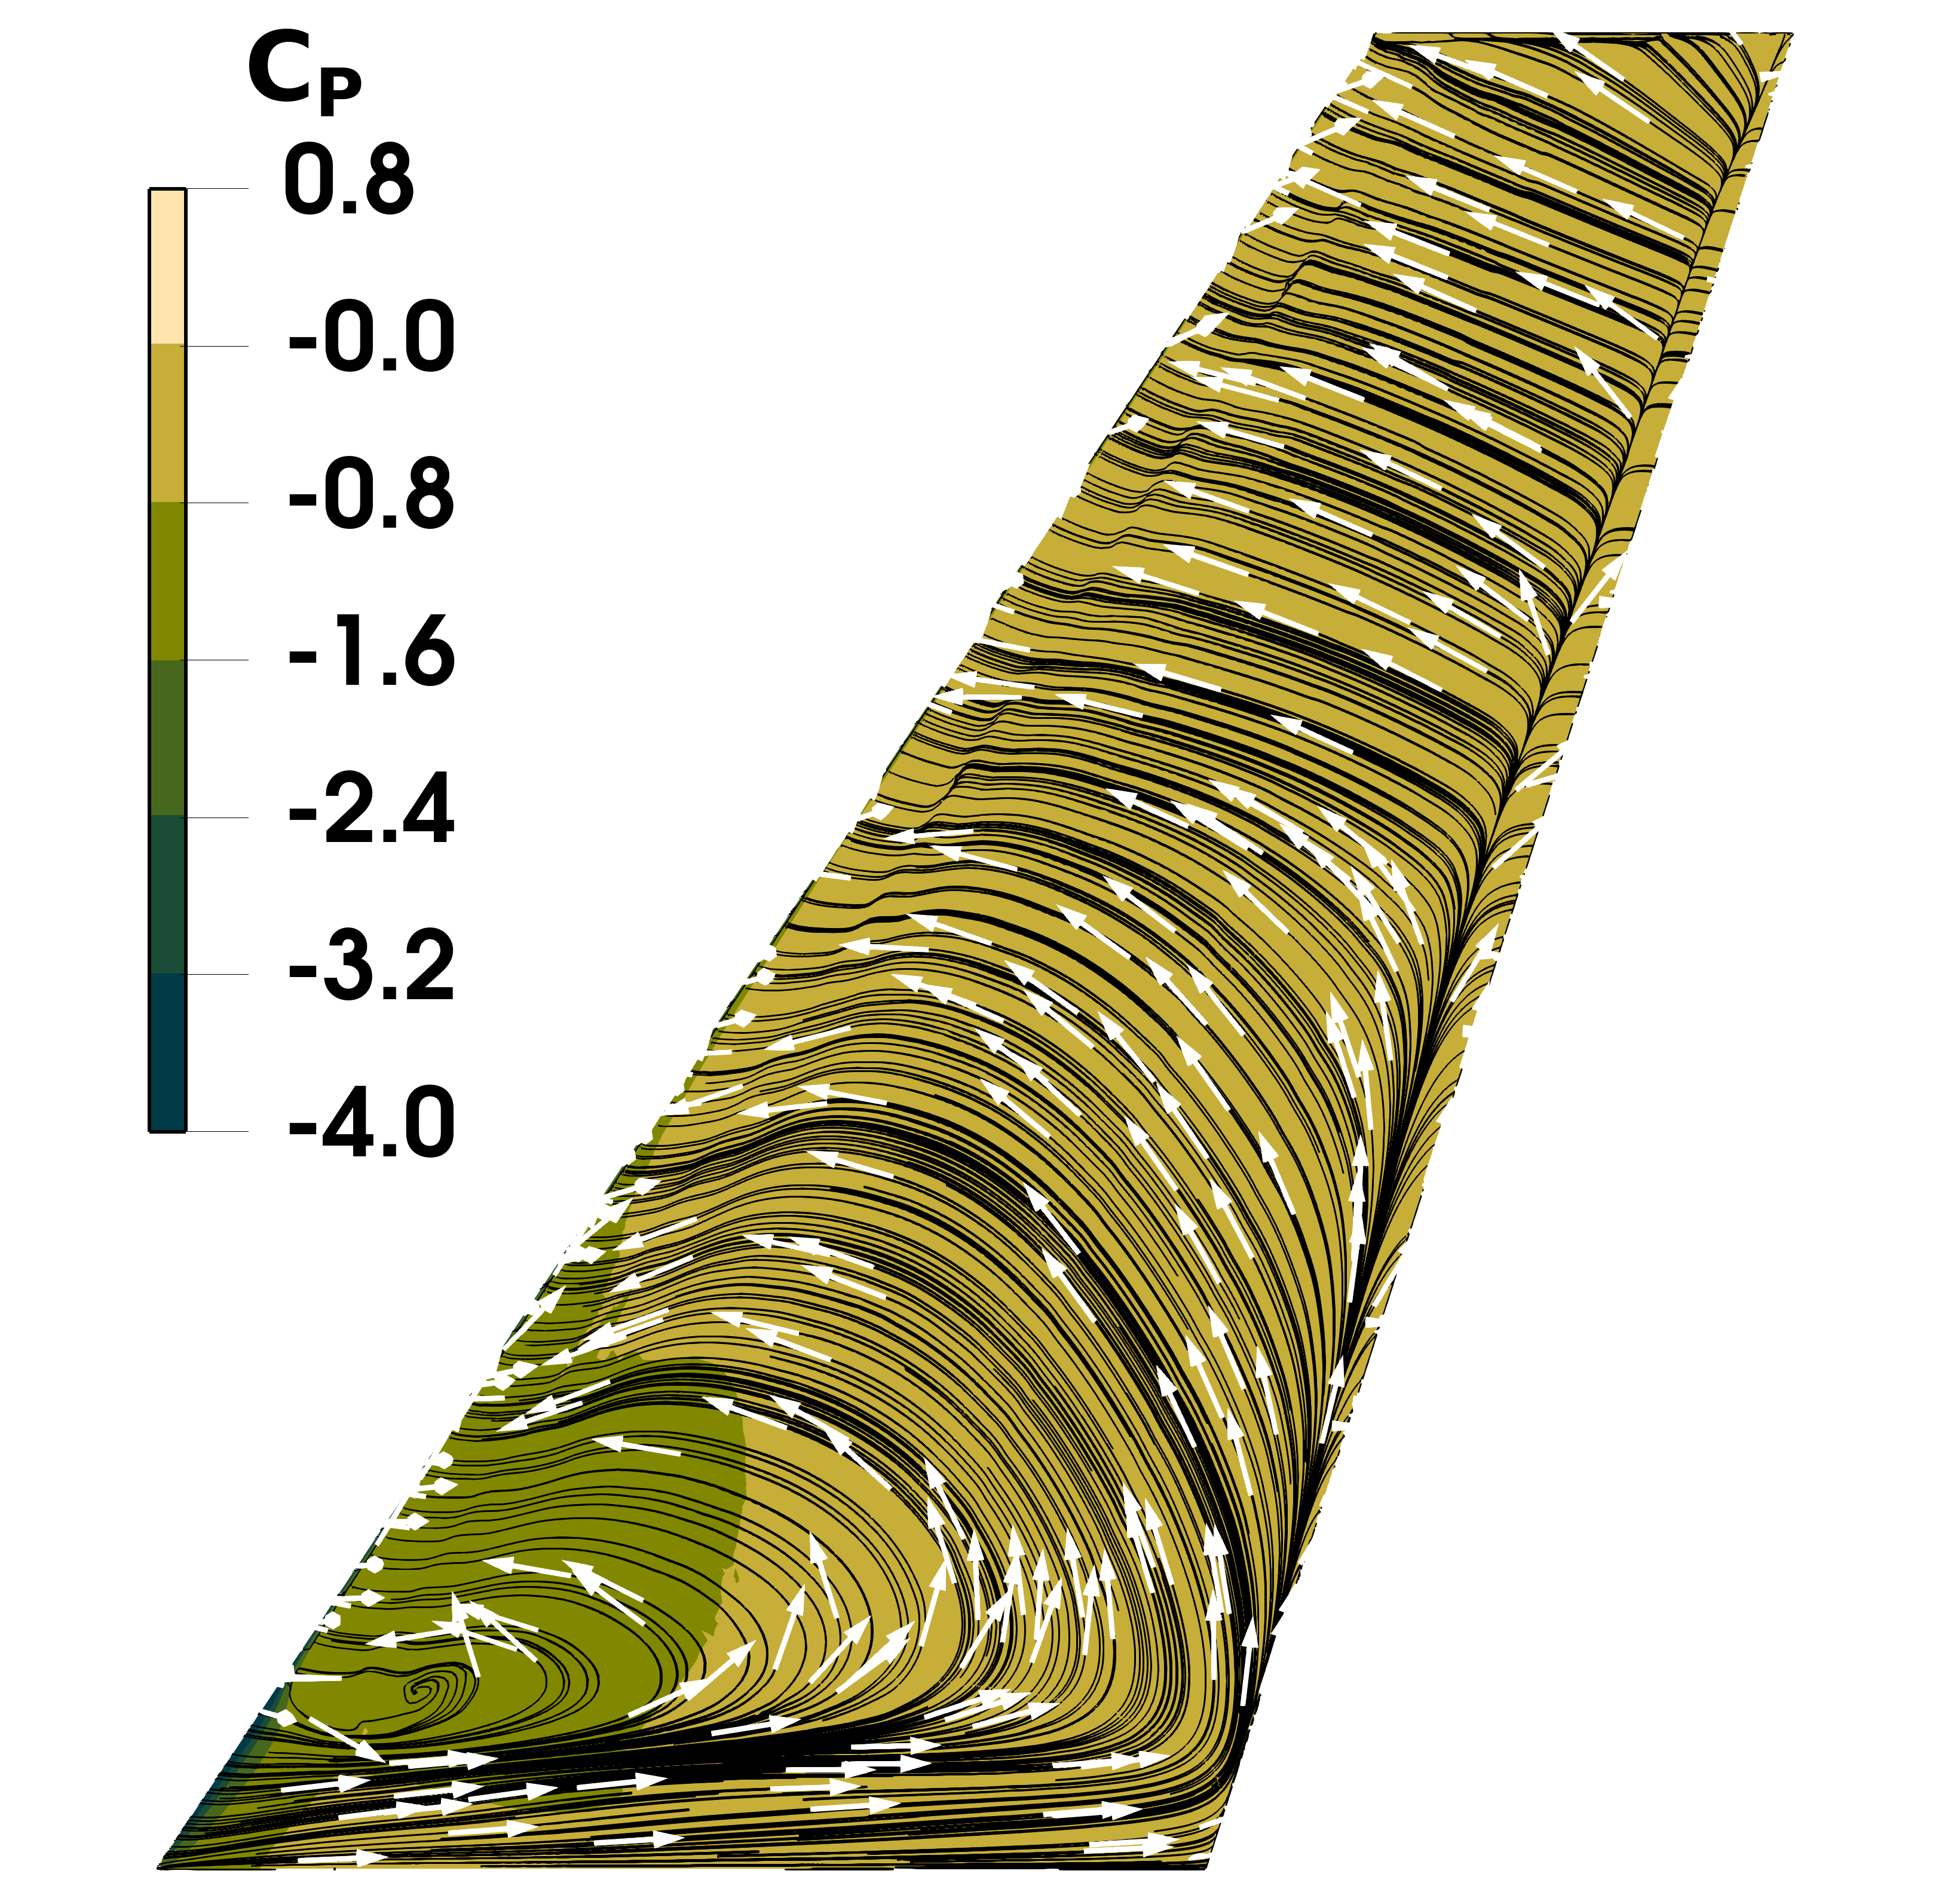
\includegraphics[width=1.2
\linewidth, height=3.6\linewidth, clip, trim={8cm 40cm 84cm 0cm}]{RefPlan_AoA_18_Delta_0_UpperSurface_CP.png}}
\\


\makecell[c]{\DeltaCaption{10}}
&
\MaskedImage[width=0.28\textwidth]{RefPlan_AoA_8_Delta_10_UpperSurface_CP.png}{%
    \maskrecttl{0.0}{0.0}{0.3}{0.63}
    \maskrecttl{0.7}{0.72}{0.26}{0.3}
    \node[] at (0.3,0.7) {\AlphaSimple{8}};
}
&
\MaskedImage[width=0.28\textwidth]{RefPlan_AoA_10_Delta_10_UpperSurface_CP.png}{%
    \maskrecttl{0.0}{0.0}{0.3}{0.63}
    \maskrecttl{0.7}{0.72}{0.26}{0.3}
    \node[] at (0.3,0.7) {\AlphaSimple{10}};
}

&
\MaskedImage[width=0.28\textwidth]{RefPlan_AoA_18_Delta_10_UpperSurface_CP.png}{%
    \maskrecttl{0.0}{0.0}{0.3}{0.63}
    \maskrecttl{0.7}{0.72}{0.26}{0.3}
    \node[] at (0.3,0.7) {\AlphaSimple{18}};
}

&
\multirow[c]{1}{*}[1.7cm]{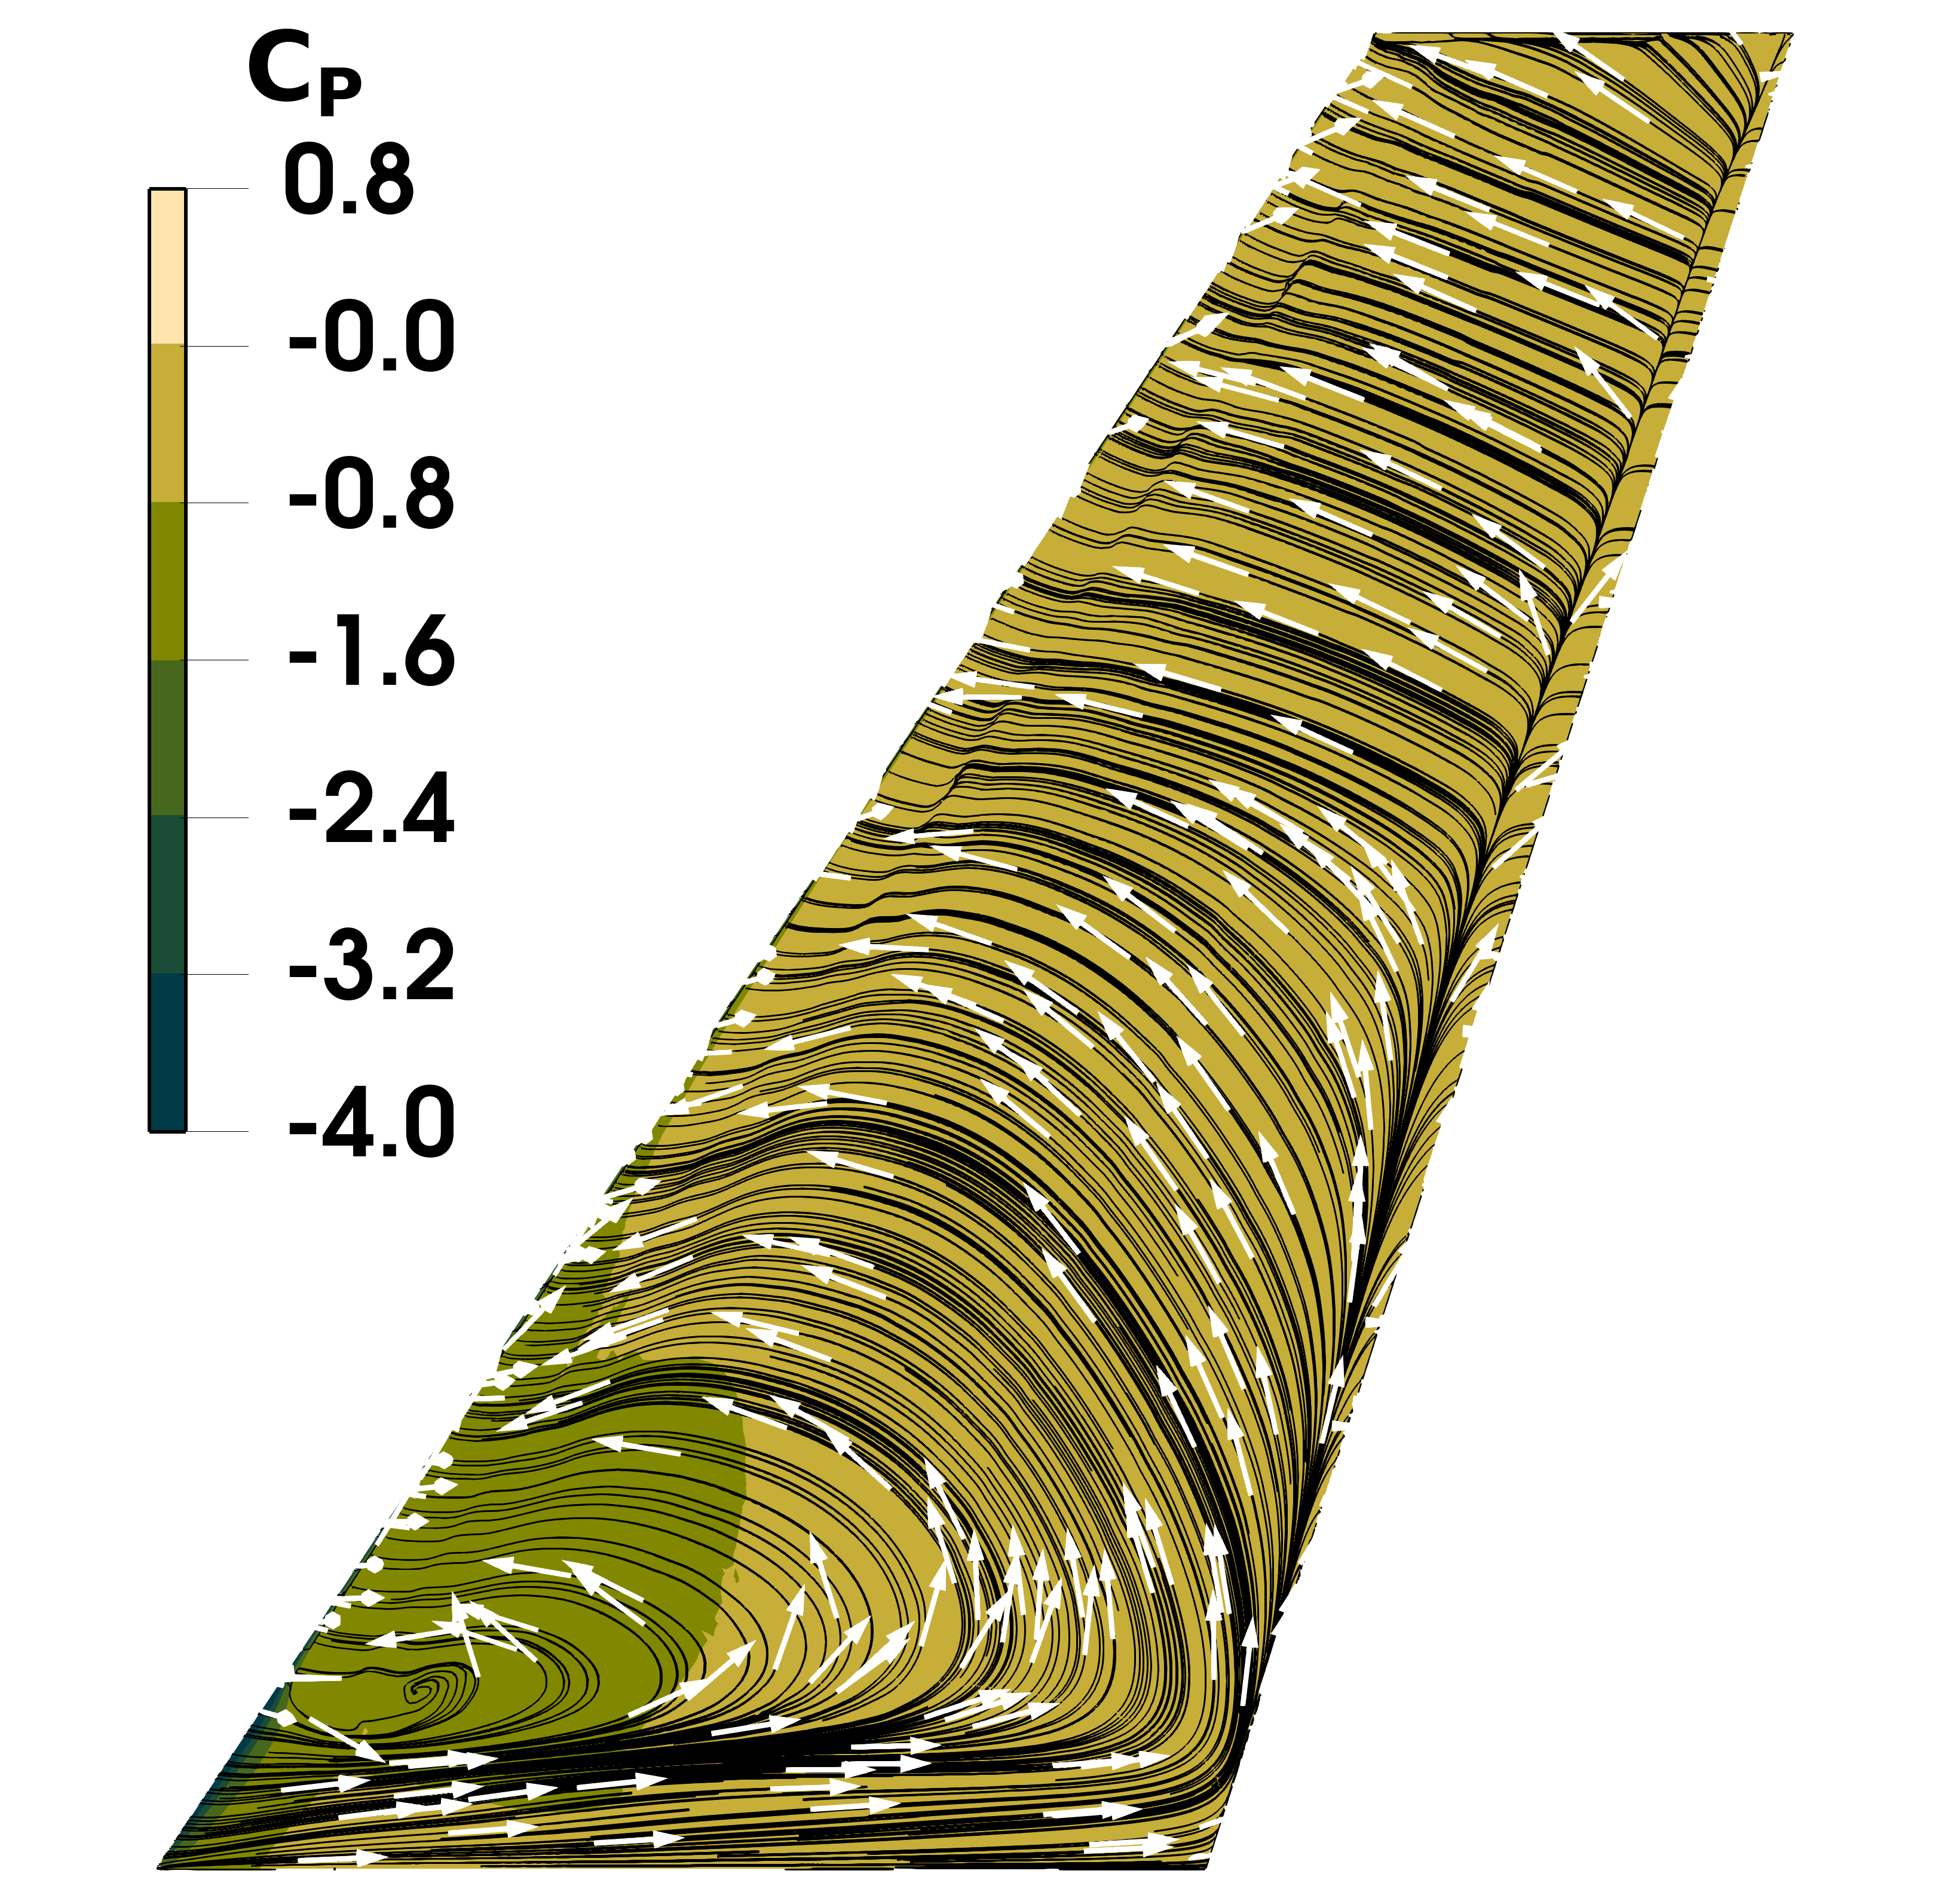
\includegraphics[width=1.2
\linewidth, height=3.6\linewidth, clip, trim={8cm 40cm 84cm 0cm}]{RefPlan_AoA_18_Delta_0_UpperSurface_CP.png}}
\\

\makecell[c]{\DeltaCaption{20}}
&
\MaskedImage[width=0.28\textwidth]{RefPlan_AoA_6_Delta_20_UpperSurface_CP.png}{%
    \maskrecttl{0.0}{0.0}{0.3}{0.63}
    \maskrecttl{0.7}{0.72}{0.26}{0.3}
    \node[] at (0.3,0.7) {\AlphaSimple{6}};
}
&
\MaskedImage[width=0.28\textwidth]{RefPlan_AoA_10_Delta_20_UpperSurface_CP.png}{%
    \maskrecttl{0.0}{0.0}{0.3}{0.63}
    \maskrecttl{0.7}{0.72}{0.26}{0.3}
    \node[] at (0.3,0.7) {\AlphaSimple{10}};
}

&
\MaskedImage[width=0.28\textwidth]{RefPlan_AoA_14_Delta_20_UpperSurface_CP.png}{%
    \maskrecttl{0.0}{0.0}{0.3}{0.63}
    \maskrecttl{0.7}{0.72}{0.26}{0.3}
    \node[] at (0.3,0.7) {\AlphaSimple{14}};
}

&
\multirow[c]{1}{*}[1.7cm]{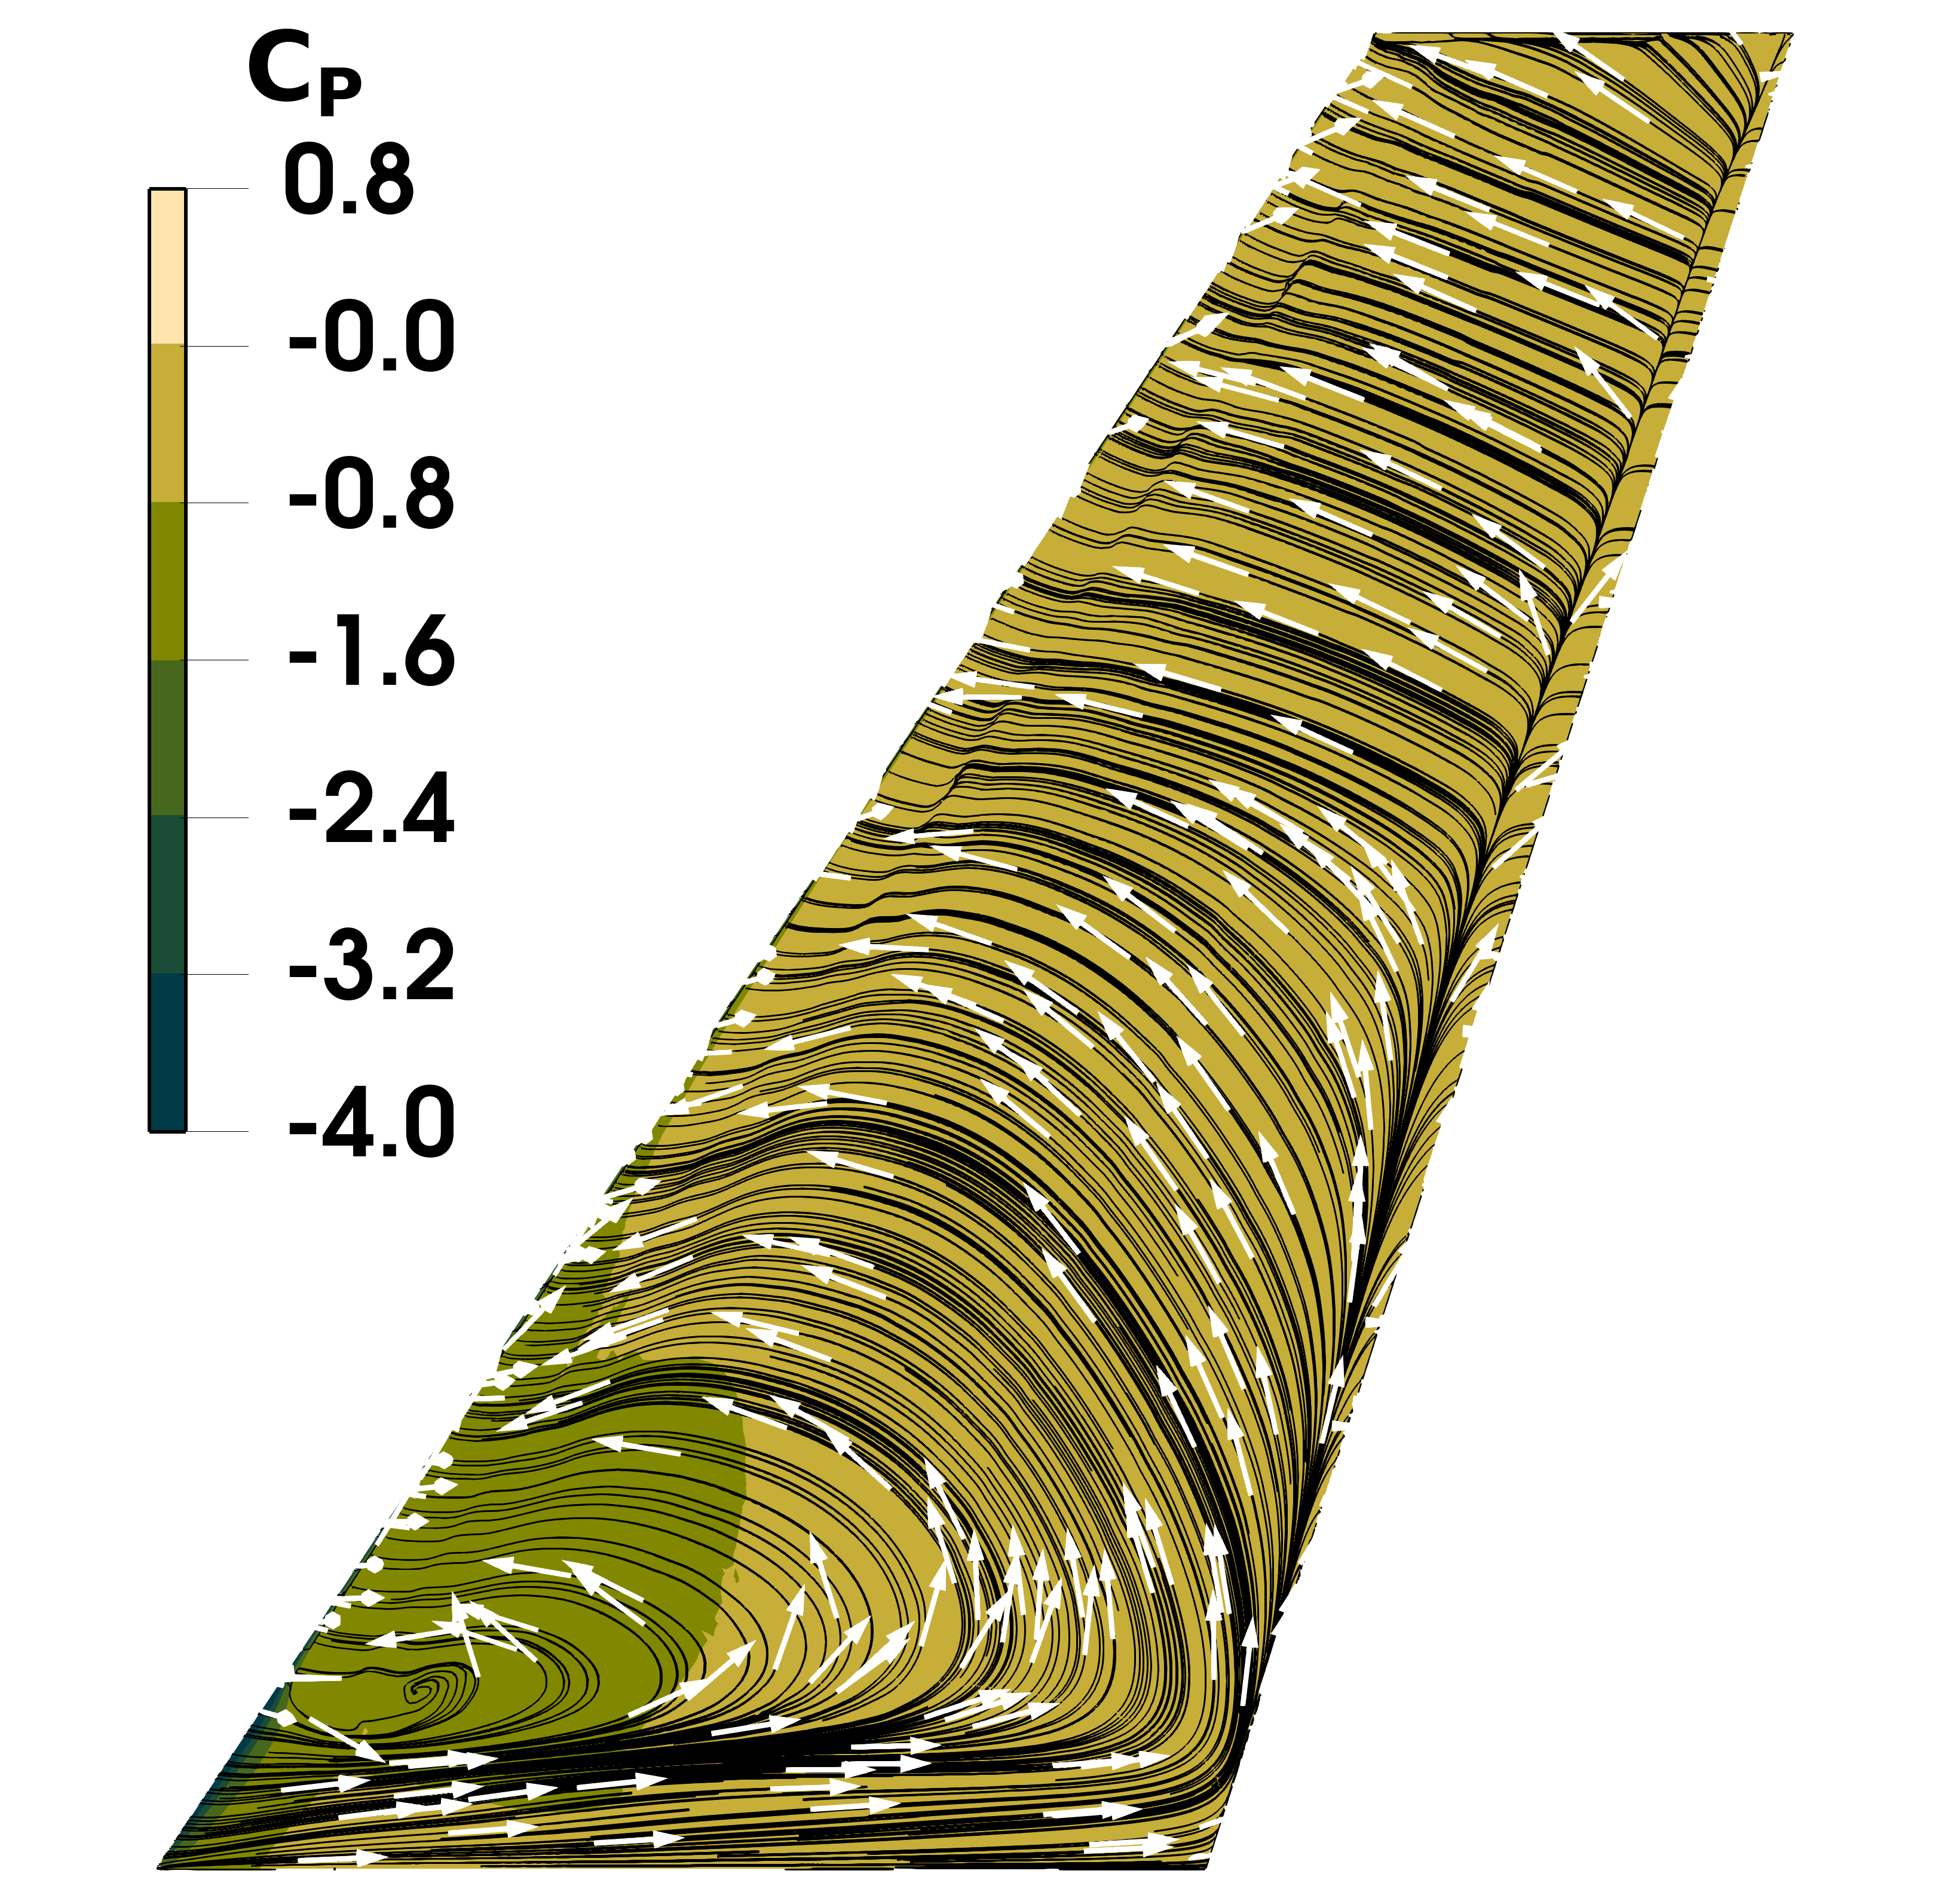
\includegraphics[width=1.2
\linewidth, height=3.6\linewidth, clip, trim={8cm 40cm 84cm 0cm}]{RefPlan_AoA_18_Delta_0_UpperSurface_CP.png}}
\\

\makecell[c]{\DeltaCaption{35}}
&
\MaskedImage[width=0.28\textwidth]{RefPlan_AoA_8_Delta_35_UpperSurface_CP.png}{%
    \maskrecttl{0.0}{0.0}{0.3}{0.63}
    \maskrecttl{0.7}{0.72}{0.26}{0.3}
    \node[] at (0.3,0.7) {\AlphaSimple{8}};
}
&
\MaskedImage[width=0.28\textwidth]{RefPlan_AoA_10_Delta_35_UpperSurface_CP.png}{%
    \maskrecttl{0.0}{0.0}{0.3}{0.63}
    \maskrecttl{0.7}{0.72}{0.26}{0.3}
    \node[] at (0.3,0.7) {\AlphaSimple{10}};
}

&
\MaskedImage[width=0.28\textwidth]{RefPlan_AoA_26_Delta_35_UpperSurface_CP.png}{%
    \maskrecttl{0.0}{0.0}{0.3}{0.63}
    \maskrecttl{0.7}{0.72}{0.26}{0.3}
    \node[] at (0.3,0.7) {\AlphaSimple{26}};
}

&
\multirow[c]{1}{*}[1.7cm]{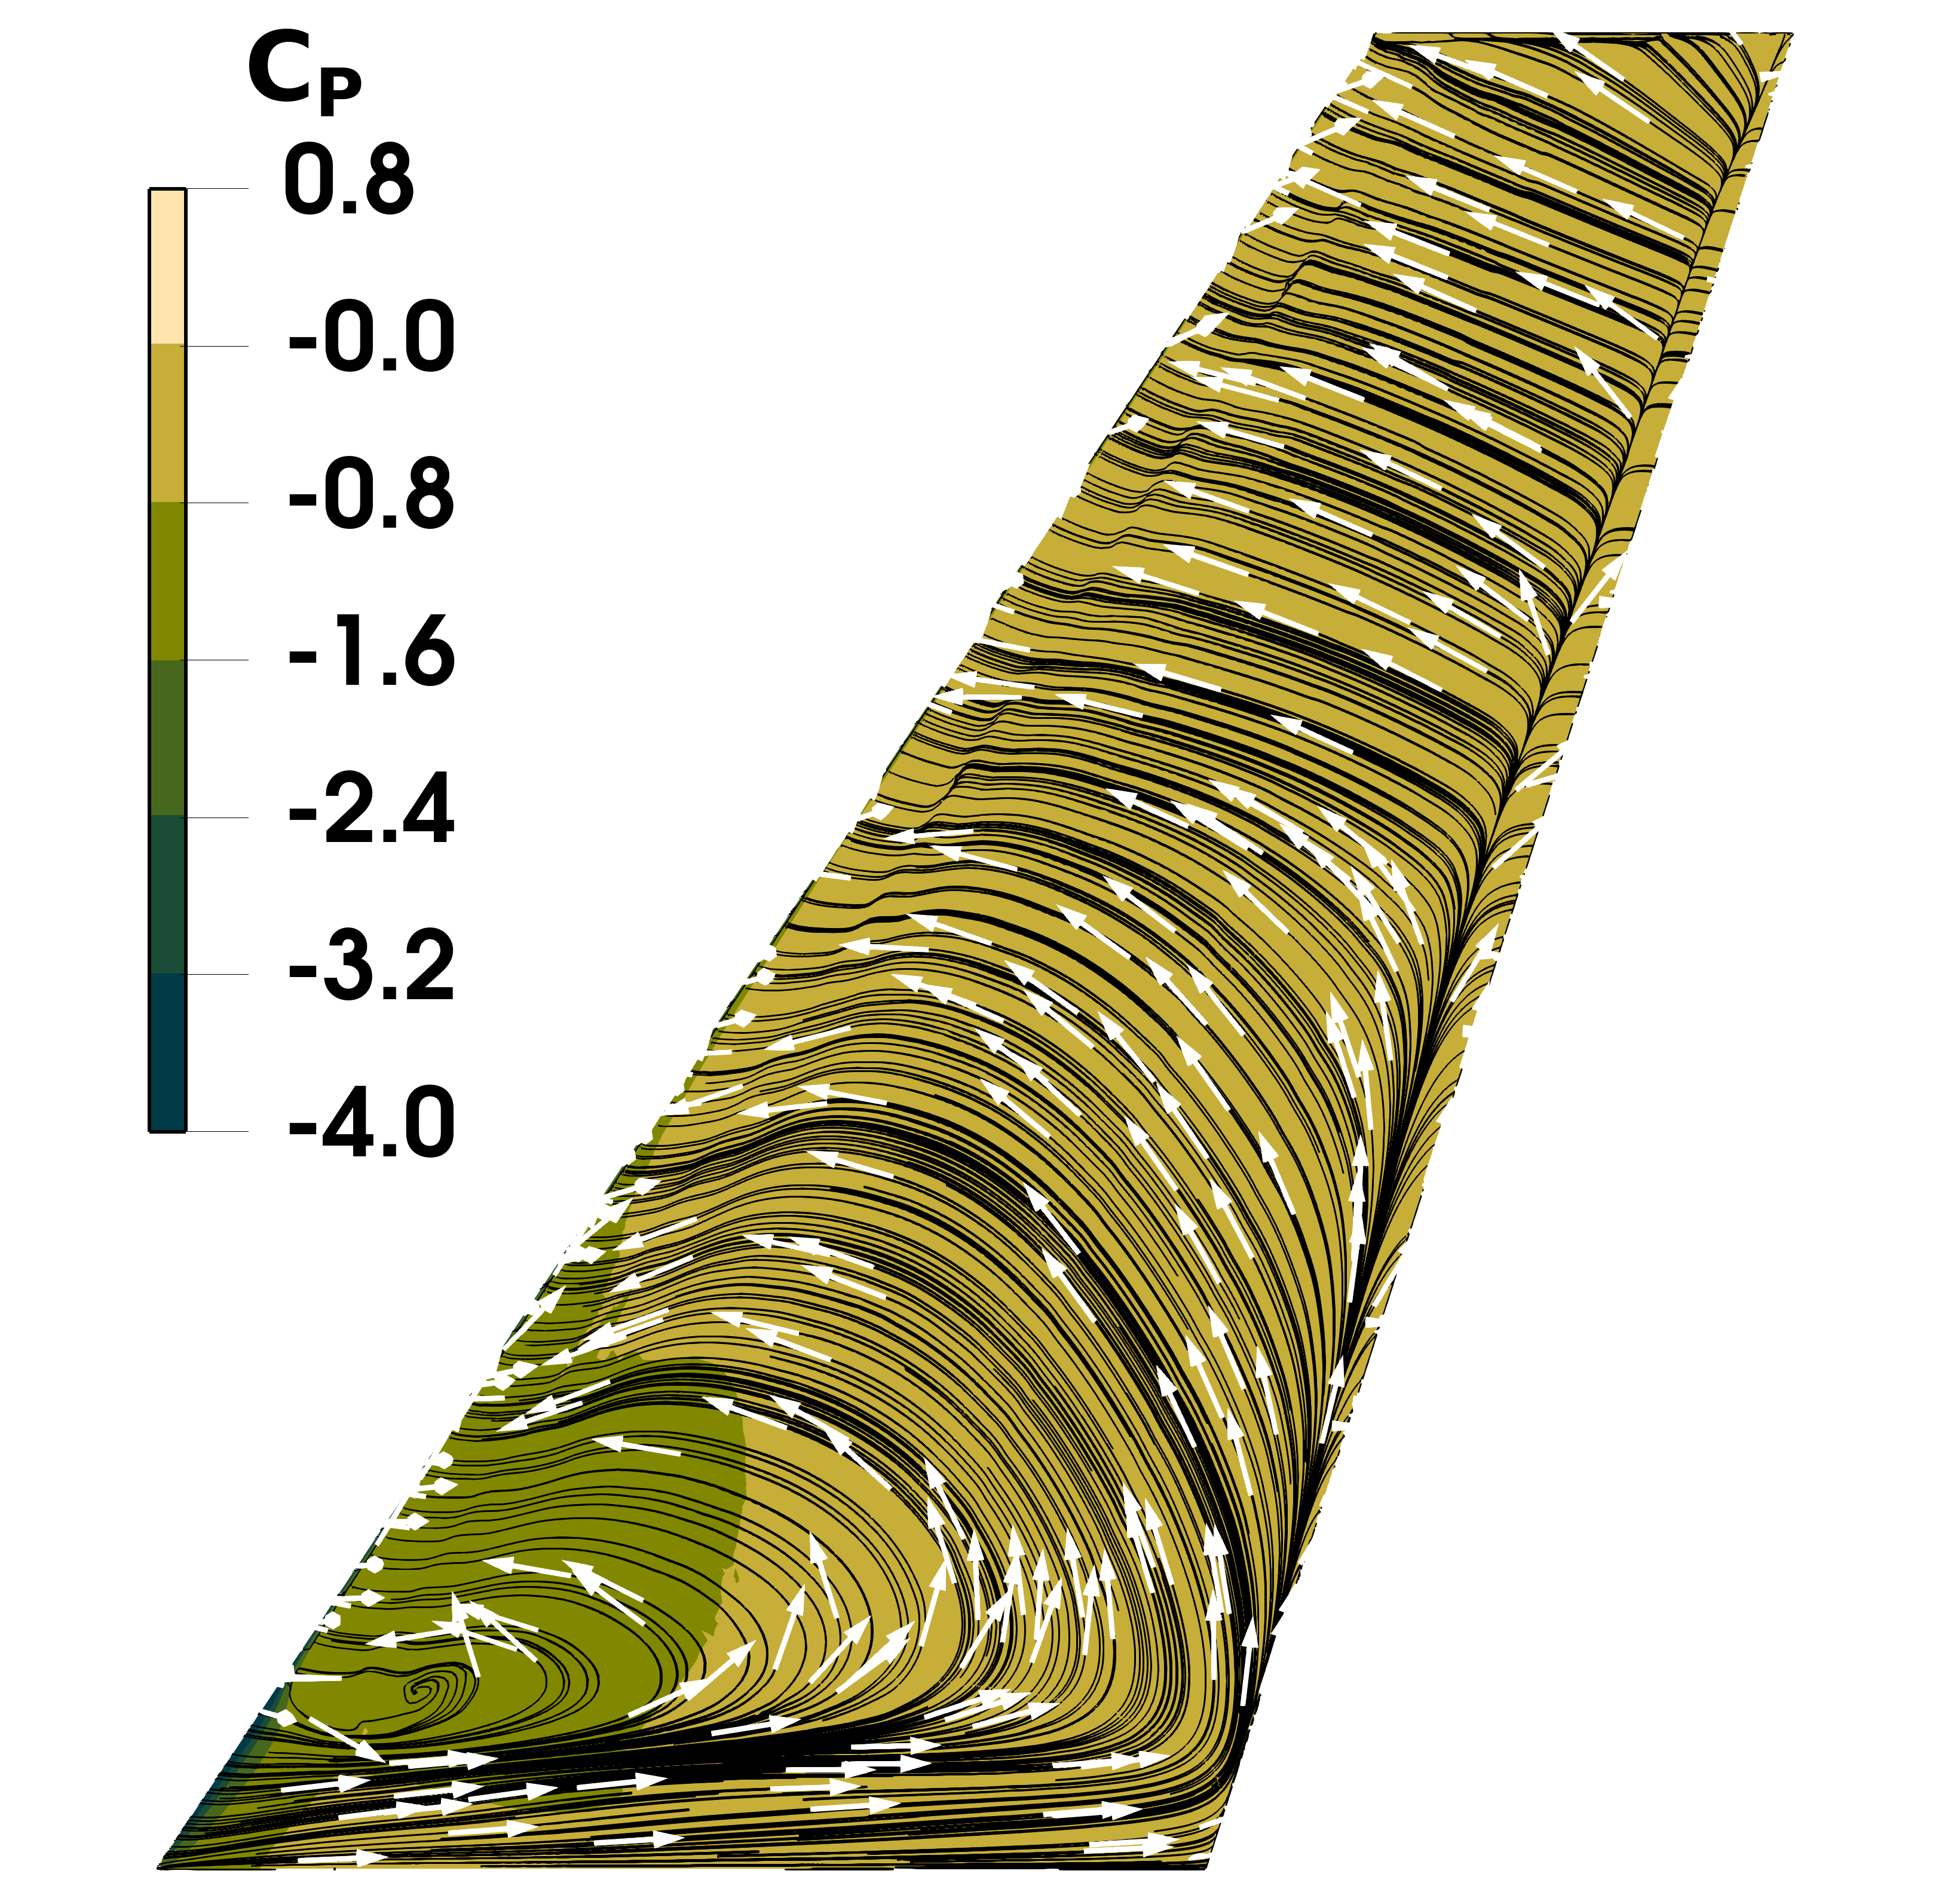
\includegraphics[width=1.2
\linewidth, height=3.6\linewidth, clip, trim={8cm 40cm 84cm 0cm}]{RefPlan_AoA_18_Delta_0_UpperSurface_CP.png}}
\\

\hline
\hline
\end{tabular}
\caption{RANS surface-flow topology at representative stages of main-surface stall for selected control deflections.}
\label{fig:FlowTopology:Delta_0_10_20_34}
\end{figure}

At the displayed maximum-lift states for the lower deflections, the fixed surface remains largely attached.
As deflection increases, a recirculating region first appears near the trailing edge and then progressively extends over the deflected control surface.
The fixed surface continues to gain lift after control-surface separation, allowing the total lift to reach a later maximum.
At \(\delta=35^\circ\), the maximum-lift state occurs when separation already affects a substantial portion of the fixed surface.
Nevertheless, the inboard region remains largely attached.
Because this region has a larger local chord due to the tapered planform, it contributes substantially to the integrated lift.

In the selected post-peak states, the RANS lift curves have undergone a marked decrease.
In the zero-deflection case, this condition is associated with a leading-edge separated region that extends over most of the span.
A local suction region persists within the separated structure, but its positive lift contribution does not compensate for the loss associated with the broader separated region. This provides a physical interpretation of the lower total lift relative to the preceding peak.
At \(\delta=10^\circ\), the separated structure shifts downstream relative to the zero-deflection case and lies closer to the hinge region.
This downstream displacement becomes more evident for \(\DeltaSimple{20}\), where the surface recirculation is concentrated over the control surface.
In both cases, the most inboard stations remain largely attached, consistent with the delayed separation observed near the root.
For the largest deflection, \(\DeltaSimple{35}\), the control surface is already separated over most of the span before the post-peak condition is reached.
The additional lift loss therefore comes from extending separation over the fixed surface rather than from the initial separation of the deflected surface.

At the later post-stall states, the separated structures have spread farther over the main surface.
For \(\delta=0^\circ\), the separated structure has moved further inboard, leaving only a narrow attached region near the root.
For the intermediate deflections, \(\DeltaSimple{10}\) and \(\DeltaSimple{20}\), the recirculating region associated with the control surface remains visible, while an additional separated region develops near the leading edge because of the larger incidence.
The resulting topology indicates that the post-stall state is governed by the interaction between the control-surface and main-surface separations.
For \(\DeltaSimple{35}\), the flow field becomes more irregular and does not exhibit a single well-defined recirculating cell.
The integrated lift remains close to the measured level despite differences in the detailed separation patterns. Matching experimental surface-flow images are not available at every displayed incidence.

Comparisons at each method's maximum lift must account for the different peak incidences.
The wind tunnel lift curves in Figure~\ref{fig:Coefficients:ExpvsNum:Delta0_10_20_34} show a gradual reduction of the \(C_L\)--\(\alpha\) slope and reach \(C_{L,\max}\) at higher incidences.
Surface-flow visualizations are available only at selected incidences.
The measured maximum lift occurs at \(\alpha=20^\circ\), \(18^\circ\), \(16^\circ\), and \(10^\circ\) for \(\delta=0^\circ\), \(10^\circ\), \(20^\circ\), and \(34^\circ\), whereas the closest available visualizations are at \(\alpha=22^\circ\), \(18^\circ\), \(18^\circ\), and \(14^\circ\).
The visualizations therefore correspond to the maximum-lift incidence for \(\delta=10^\circ\) and to incidences \(2^\circ\)--\(4^\circ\) beyond it for the other deflections.

Figure~\ref{fig:FlowTopology:RANSVsExp} is therefore organized to separate the discrepancy in maximum-lift incidence from the discrepancy in separated-flow topology.
For each deflection, the first column reports the RANS topology at the RANS maximum-lift condition, the second column reports the wind tunnel visualization closest to the experimental maximum-lift incidence, and the third column reports the RANS topology at the same incidence as the corresponding wind tunnel visualization.
The panel labels give the actual incidences. Rows are indexed by the measured deflections; the last row compares \(34^\circ\) experimentally with \(35^\circ\) numerically.

\begin{figure}[h!]
\centering
\begin{tabular}{>{\centering\arraybackslash}m{1.2cm}>{\centering\arraybackslash}m{4cm}>{\centering\arraybackslash}m{4cm}>{\centering\arraybackslash}m{4cm}}
\hline
\hline
&
\textbf{3D RANS}
&
\textbf{Wind Tunnel}
&
\textbf{3D RANS (@$\alpha_{WT}$)}
\\
\hline

\makecell[c]{\DeltaCaption{0}}
&
\MaskedImage[width=0.28\textwidth]{RefPlan_AoA_12_Delta_0_UpperSurface_CP.png}{%
    \maskrecttl{0.0}{0.0}{0.3}{0.63}
    \maskrecttl{0.7}{0.72}{0.26}{0.3}
    \node[] at (0.3,0.7) {\AlphaSimple{12}};
}
&
\begin{tikzpicture}
    \node[anchor=south west, inner sep=0] (img) at (0,0)
        {\reflectbox{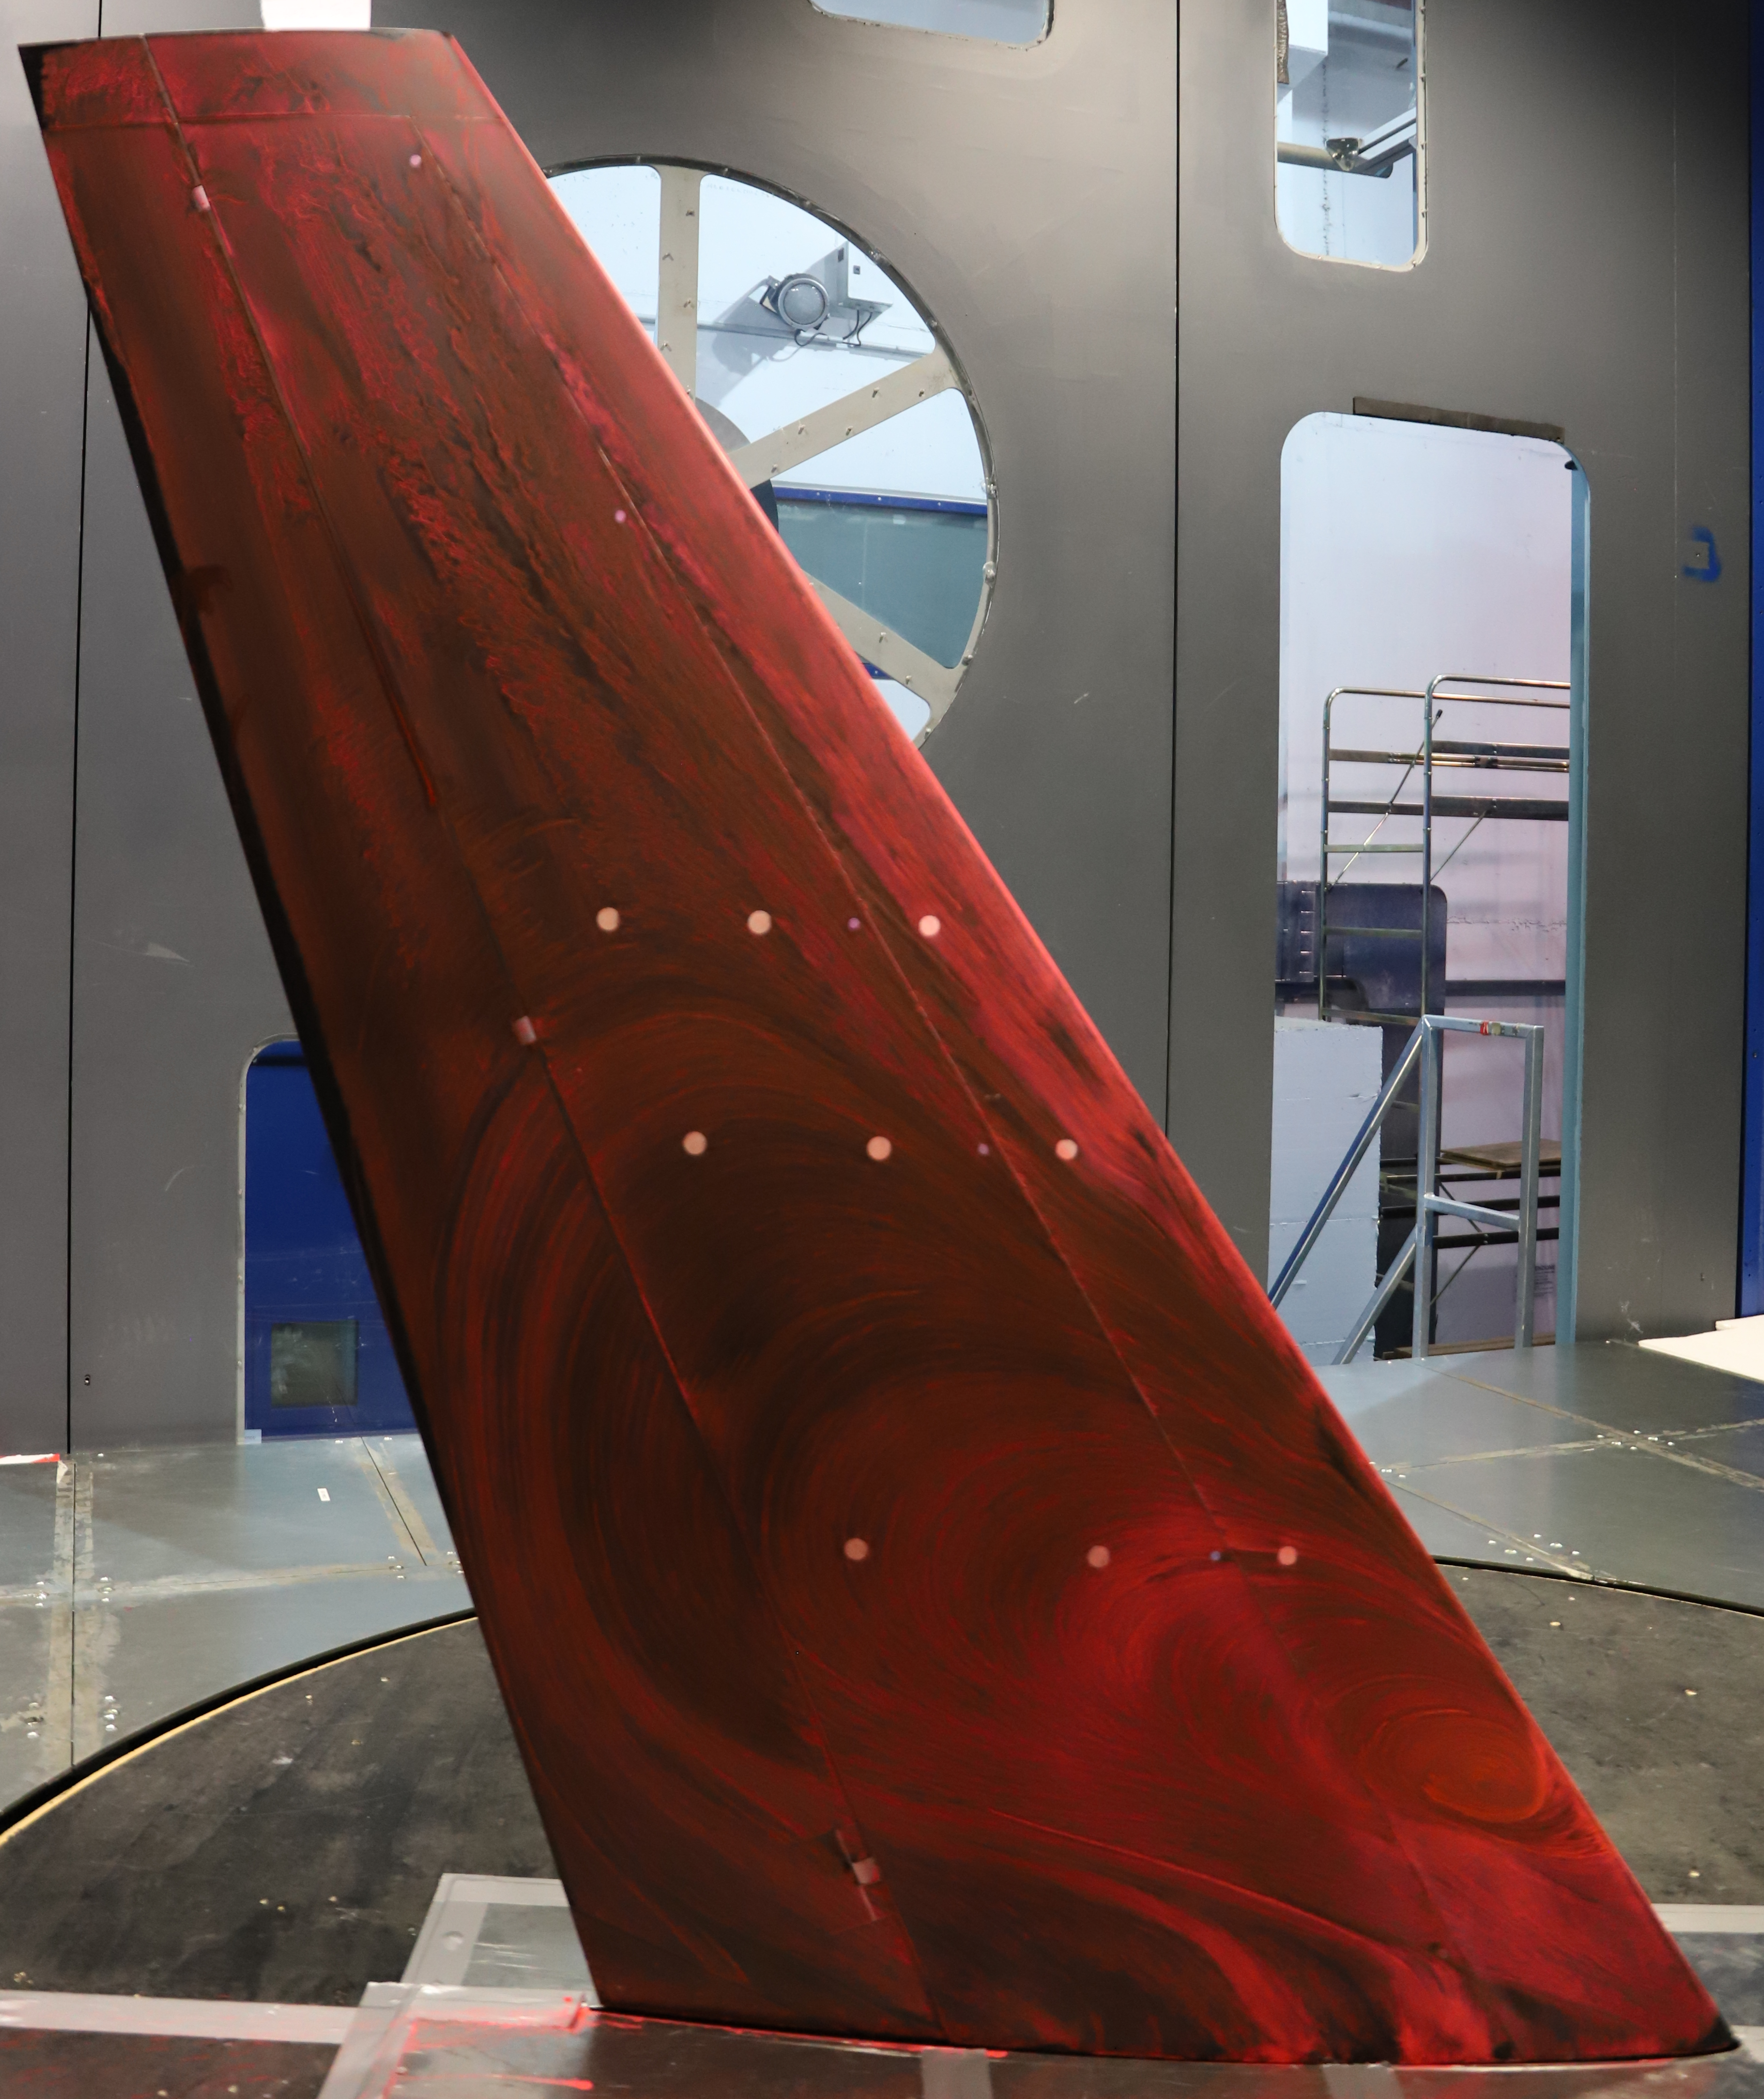
\includegraphics[width=0.24\textwidth]{AoA_22_delta_0.png}}};
    \begin{scope}[x={(img.south east)}, y={(img.north west)}]
        \node[fill=white] at (0.3, 0.7) {\AlphaSimple{22}};
    \end{scope}
\end{tikzpicture}%
&
\MaskedImage[width=0.28\textwidth]{RefPlan_AoA_22_Delta_0_UpperSurface_CP.png}{%
    \maskrecttl{0.0}{0.0}{0.3}{0.63}
    \maskrecttl{0.7}{0.72}{0.26}{0.3}
    \node[] at (0.3,0.7) {\AlphaSimple{22}};
}

\\


\makecell[c]{\DeltaCaption{10}}
&
\MaskedImage[width=0.28\textwidth]{RefPlan_AoA_8_Delta_10_UpperSurface_CP.png}{%
    \maskrecttl{0.0}{0.0}{0.3}{0.63}
    \maskrecttl{0.7}{0.72}{0.26}{0.3}
    \node[] at (0.3,0.7) {\AlphaSimple{8}};
}
&
\begin{tikzpicture}
    \node[anchor=south west, inner sep=0] (img) at (0,0)
        {\reflectbox{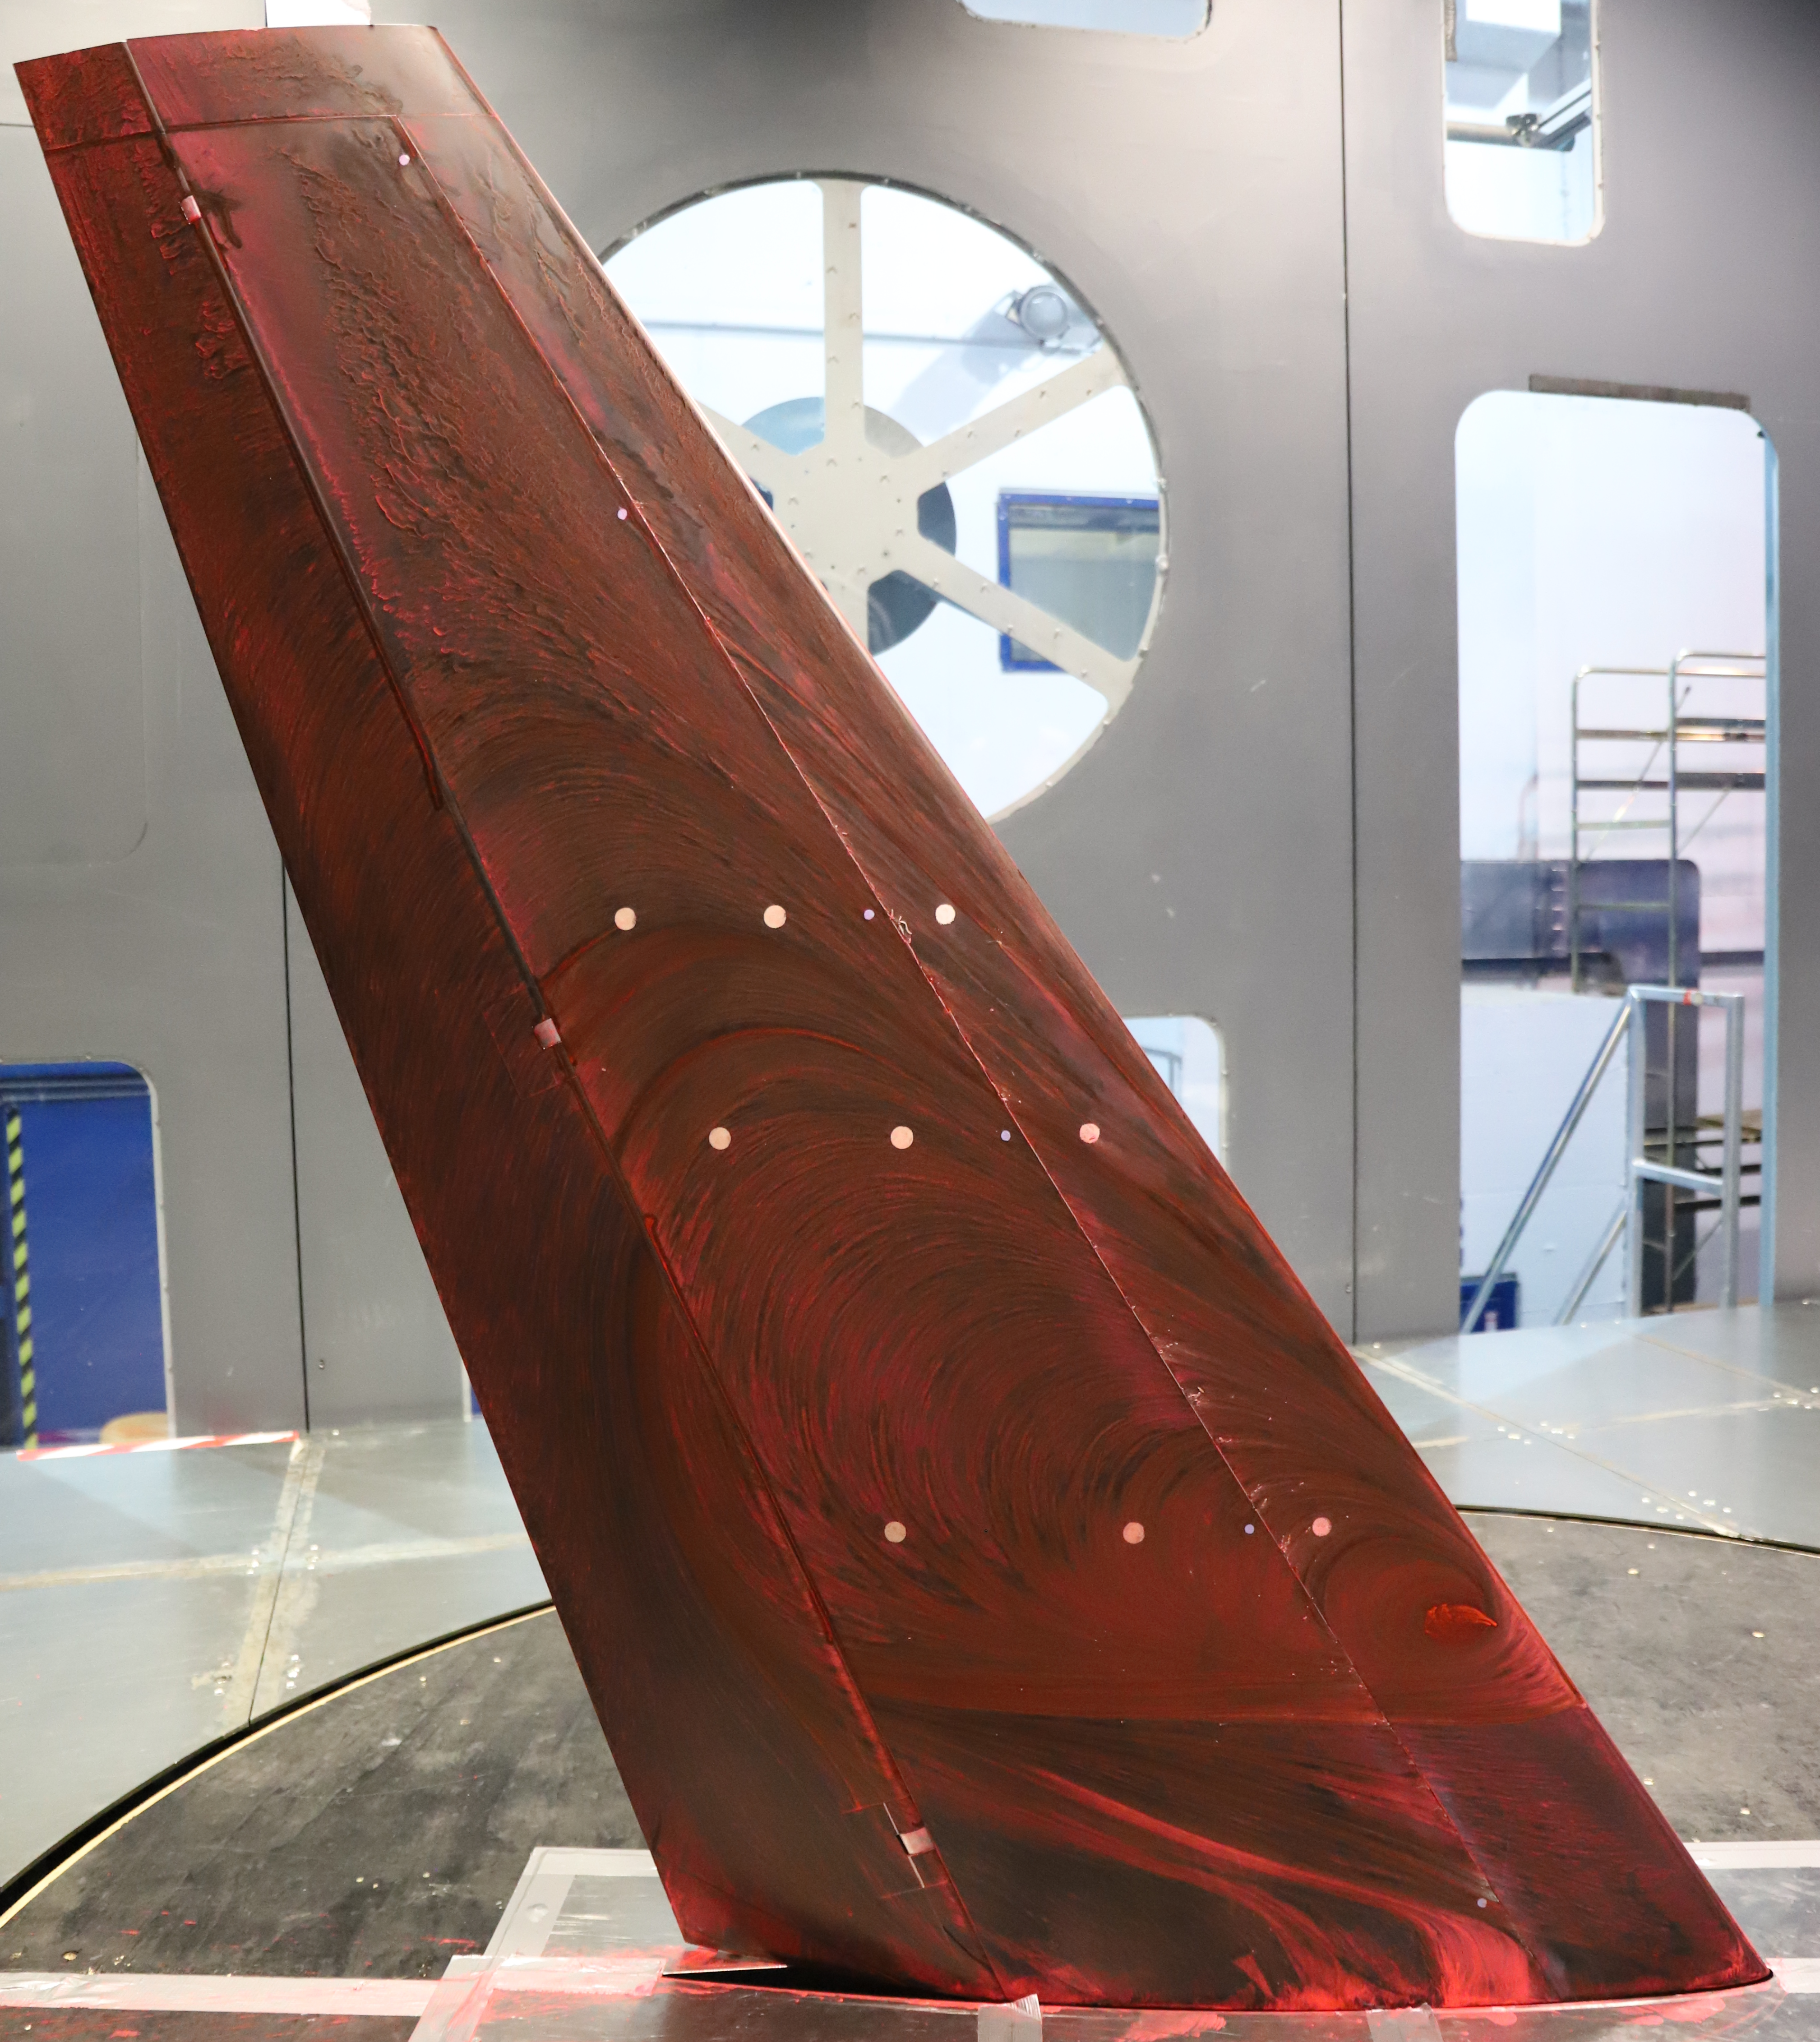
\includegraphics[width=0.24\textwidth]{AoA_18_Delta_-10.png}}};
    \begin{scope}[x={(img.south east)}, y={(img.north west)}]
        \node[fill=white] at (0.3, 0.7) {\AlphaSimple{18}};
    \end{scope}
\end{tikzpicture}%
&
\MaskedImage[width=0.28\textwidth]{RefPlan_AoA_18_Delta_10_UpperSurface_CP.png}{%
    \maskrecttl{0.0}{0.0}{0.3}{0.63}
    \maskrecttl{0.7}{0.72}{0.26}{0.3}
    \node[] at (0.3,0.7) {\AlphaSimple{18}};
}

\\

\makecell[c]{\DeltaCaption{20}}
&
\MaskedImage[width=0.28\textwidth]{RefPlan_AoA_6_Delta_20_UpperSurface_CP.png}{%
    \maskrecttl{0.0}{0.0}{0.3}{0.63}
    \maskrecttl{0.7}{0.72}{0.26}{0.3}
    \node[] at (0.3,0.7) {\AlphaSimple{6}};
}
&
\begin{tikzpicture}
    \node[anchor=south west, inner sep=0] (img) at (0,0)
        {\reflectbox{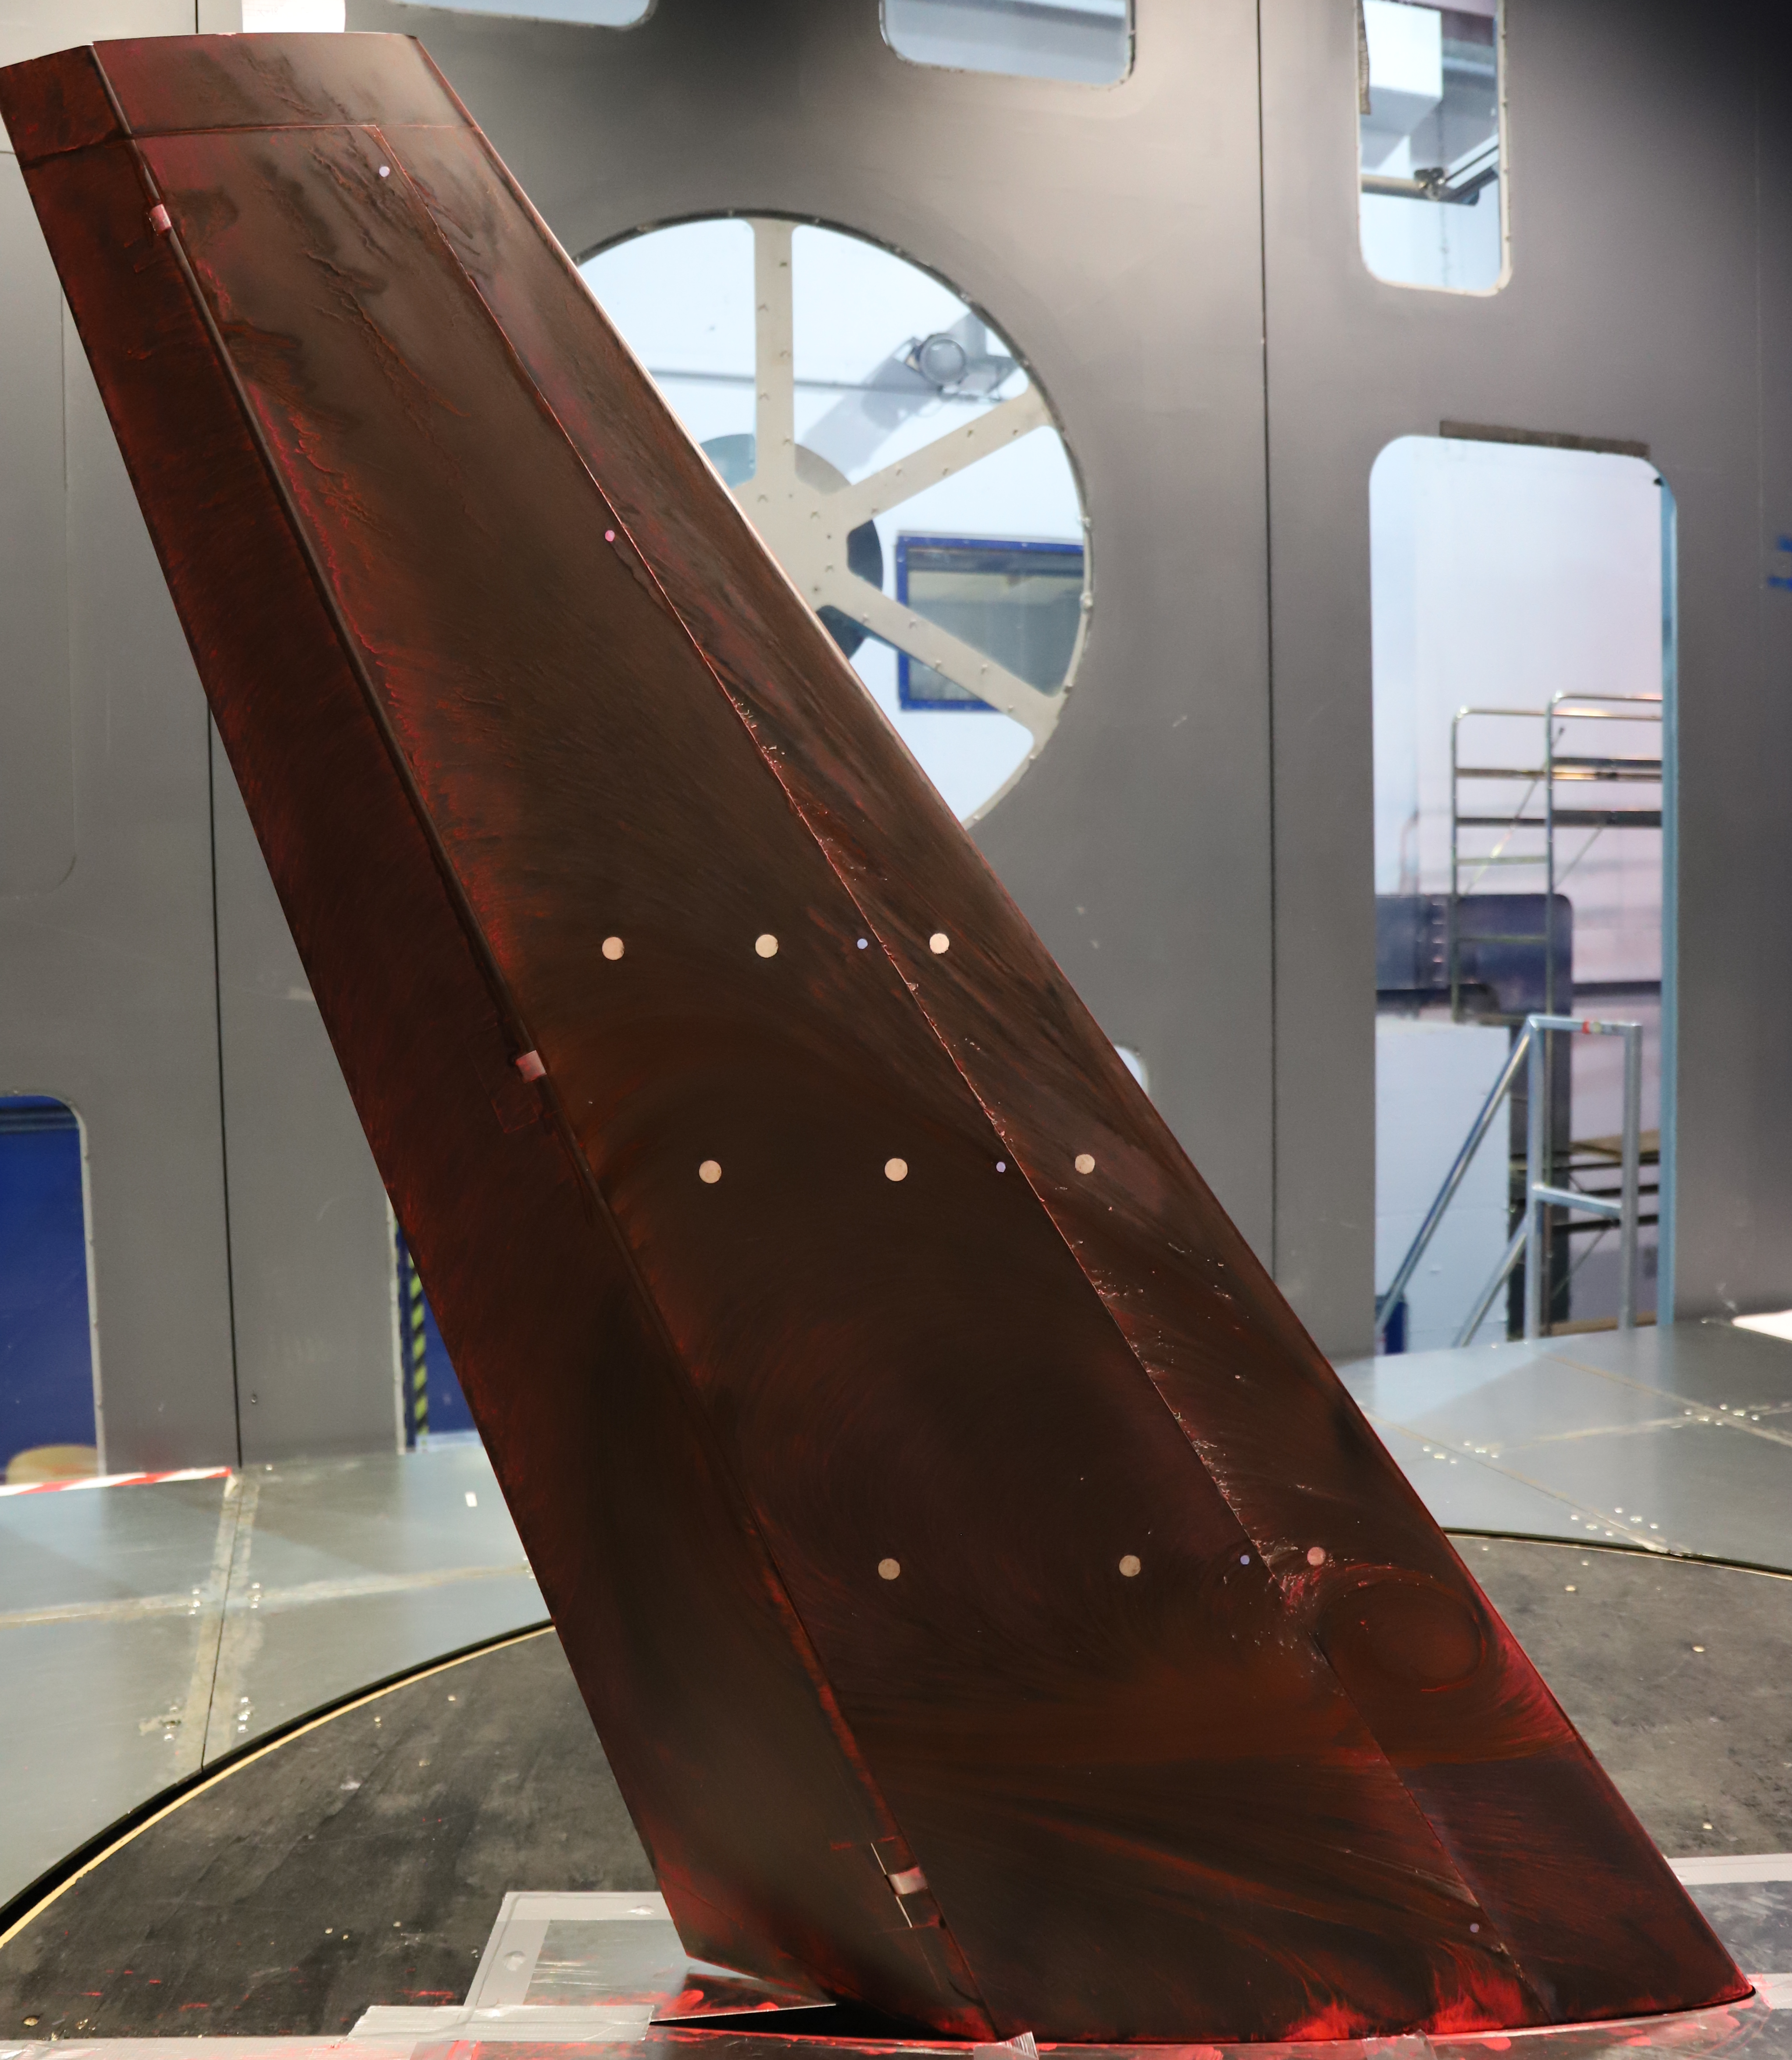
\includegraphics[width=0.24\textwidth]{AoA_18_Delta_-20.png}}};
    \begin{scope}[x={(img.south east)}, y={(img.north west)}]
        \node[fill=white] at (0.3, 0.7) {\AlphaSimple{18}};
    \end{scope}
\end{tikzpicture}%
&
\MaskedImage[width=0.28\textwidth]{RefPlan_AoA_18_Delta_20_UpperSurface_CP.png}{%
    \maskrecttl{0.0}{0.0}{0.3}{0.63}
    \maskrecttl{0.7}{0.72}{0.26}{0.3}
    \node[] at (0.3,0.7) {\AlphaSimple{18}};
}
\\

\makecell[c]{\DeltaCaption{34}}
&
\MaskedImage[width=0.28\textwidth]{RefPlan_AoA_8_Delta_35_UpperSurface_CP.png}{%
    \maskrecttl{0.0}{0.0}{0.3}{0.63}
    \maskrecttl{0.7}{0.72}{0.26}{0.3}
    \node[] at (0.3,0.7) {\AlphaSimple{8}};
}
&
\begin{tikzpicture}
    \node[anchor=south west, inner sep=0] (img) at (0,0)
        {\reflectbox{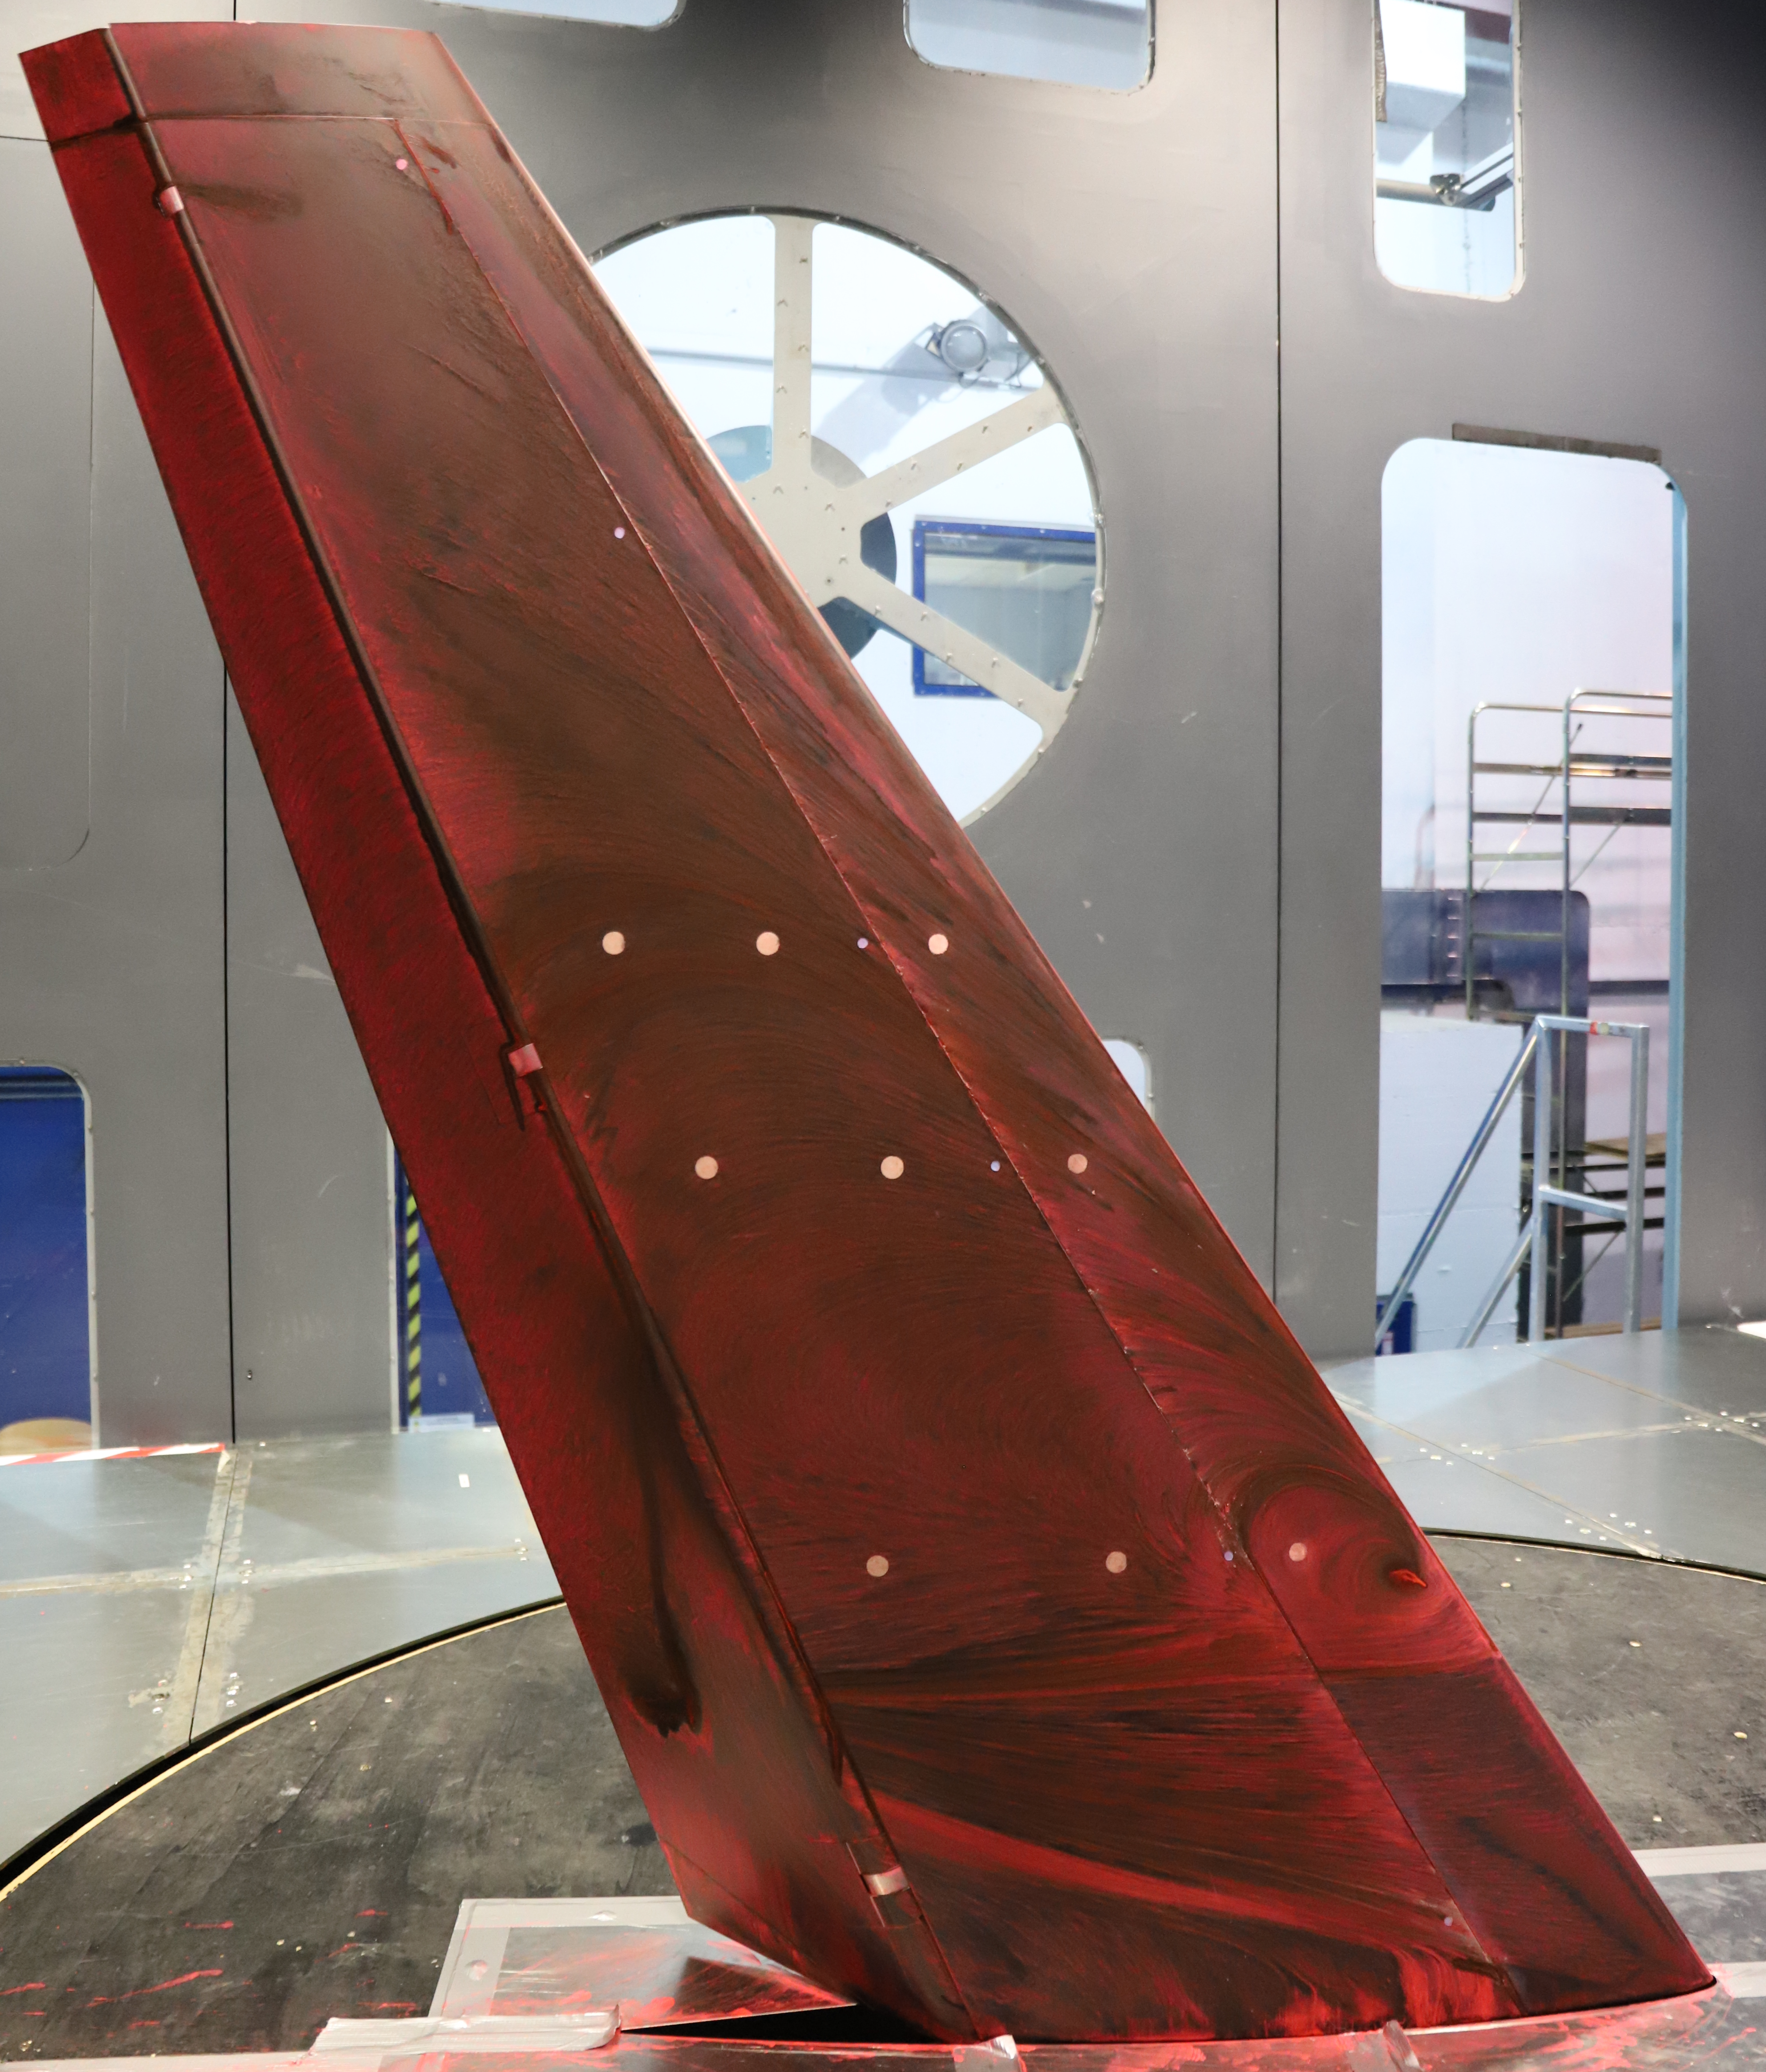
\includegraphics[width=0.24\textwidth]{AoA_14_Delta_-34.png}}};
    \begin{scope}[x={(img.south east)}, y={(img.north west)}]
        \node[fill=white] at (0.3, 0.7) {\AlphaSimple{14}};
    \end{scope}
\end{tikzpicture}%
&
\MaskedImage[width=0.28\textwidth]{RefPlan_AoA_14_Delta_35_UpperSurface_CP.png}{%
    \maskrecttl{0.0}{0.0}{0.3}{0.63}
    \maskrecttl{0.7}{0.72}{0.26}{0.3}
    \node[] at (0.3,0.7) {\AlphaSimple{14}};
}

\\

\hline
\hline
\end{tabular}
\caption{Experimental surface-flow visualizations and RANS topology near maximum lift and at high incidence.}
\label{fig:FlowTopology:RANSVsExp}
\end{figure}

Figure~\ref{fig:FlowTopology:RANSVsExp} shows that separated flow covers a substantial portion of the tailplane at or shortly after the experimental maximum-lift incidence.
This is consistent with the gradual reduction of the experimental \(C_L\)--\(\alpha\) slope before \(C_{L,\max}\).
At the lower deflections, the RANS skin-friction patterns change rapidly after the computed lift peak (Fig.~\ref{fig:FlowTopology:Delta_0_10_20_34}). The experimental and numerical maximum-lift states therefore need not have comparable separation patterns.

When the RANS solution is evaluated at the same incidence as the wind tunnel visualization, the predicted flow topology becomes more similar to the experimental one.
In both datasets, the high-incidence state shows extensive separation and recirculating surface-flow patterns on the suction side.
However, the RANS-separated structure is generally located farther inboard than in the wind tunnel visualization.
This displacement is consistent with the different root boundary conditions. The floor boundary layer in the experiment may alter the inboard development of separation and the spanwise position of the separated structure, whereas the numerical symmetry plane excludes this boundary layer. This is a possible explanation rather than an isolated causal result; turbulence modeling and the steady-flow assumption may also contribute.

Overall, the comparison shows that RANS reproduces the main high-incidence separated-flow pattern observed in the wind tunnel, but predicts its development too abruptly and with the dominant separated structure displaced inboard.
The surface topologies thus support the interpretation of a more abrupt numerical stall mechanism and a more gradual experimental progression.


\subsection{Regime-dependent model accuracy and multi-fidelity implications}
\label{sec:model_accuracy_results}

The mechanisms governing aerodynamic loading change as separation develops over the control surface and then the fixed surface, so numerical-model accuracy depends on the flow regime. Table~\ref{tab:model_validity_summary} summarizes the observed agreement for each flow regime.
The assessment is qualitative and specific to this geometry and test matrix; application-dependent error tolerances would be needed to define a quantitative validity envelope.

\begin{table}[htbp]
    \centering
    \caption{Qualitative regime-dependent assessment of the DUST lifting-line and RANS predictions.}
    \label{tab:model_validity_summary}
    \begin{tabularx}{\linewidth}{>{\raggedright\arraybackslash}X>{\raggedright\arraybackslash}X>{\raggedright\arraybackslash}X>{\raggedright\arraybackslash}X}
        \hline
        \hline
        Regime
        & Dominant physics
        & DUST lifting line
        & RANS \\
        \hline
        Attached flow
        & Mostly linear loading
        & Good \(C_L\) trends; weaker \(C_{M_y}\)
        & Good agreement for \(C_L\) and \(C_D\); closer \(C_{M_y}\) relative to lifting line \\
        Control-surface separation
        & Local nonlinear response over the deflected surface
        & Larger onset and moment discrepancies
        & Captures the trend, but the onset may be shifted \\
        Main-surface stall
        & Rapid growth of separation over the fixed surface
        & Not recommended for quantitative prediction
        & Captures the main mechanism, but predicts a sharper stall transition \\
        Deep post-stall
        & Large-scale separated and vortical flow
        & Not recommended for quantitative prediction
        & Qualitative topology agreement; inboard displacement remains \\
        \hline
        \hline
    \end{tabularx}
\end{table}


For preliminary exploration, the lifting-line model provides useful lift trends in attached and weakly nonlinear conditions. Its larger pitching-moment discrepancies indicate that acceptable integrated lift alone is insufficient for assessing control-induced load redistribution.
Once control-surface separation develops, the RANS load decomposition provides a more detailed physical interpretation of the nonlinear response, although the predicted incidence of the loading change differs from the measurements.
In the main-stall and post-stall regimes, RANS remains informative for the broad separated-flow pattern and retained lift level.

\section{Conclusions}
\label{sec:conclusions}

A positively swept, zero-dihedral tailplane equipped with a full-span trailing-edge control surface was investigated using a multi-fidelity numerical--experimental approach.
Wind tunnel measurements, a nonlinear lifting-line model, and three-dimensional RANS simulations were compared over the full available incidence--deflection range.

A positive control deflection shifts the lift curve upward by increasing effective camber, but it also raises the adverse pressure gradient downstream of the hinge line. On the positive-incidence branch of the cases examined, separation consequently develops over the control surface before the fixed surface reaches its lift peak. The incidence at which control-surface separation affects the lift curve decreases as deflection increases.
Because the fixed surface carries most of the lift and remains largely attached, the global lift recovers and continues to grow after the control surface separates.
Control-surface separation thus appears as a local change in the lift and pitching-moment slopes well before maximum lift.
At the largest numerical setting, \(\delta=35^\circ\), the RANS control surface is separated over a broad incidence range.
Its contribution then dominates the drag in the range where the fixed surface is attached, increasing the minimum drag and causing the global drag curve to depart from the parabolic attached-flow trend.

Control-surface separation also reduces control effectiveness.
Over the common regular-response range \(-10^\circ\leq\alpha\leq-4^\circ\), measured mean lift effectiveness decreases by approximately \(6\%\) between the first two deflection intervals, while the magnitude of mean moment effectiveness changes by approximately \(2\%\).
A larger reduction occurs as incidence increases: for \([10^\circ,20^\circ]\), the measured lift effectiveness falls by approximately a factor of two between \(\alpha=-4^\circ\) and \(\alpha=0^\circ\), when the control surface separates.
The RANS mean pitching-moment effectiveness differs from the measured central values by less than \(1\%\) over the common negative-incidence range, but it overpredicts the lift effectiveness by \(15\)--\(24\%\) and delays the onset of control-surface separation.
The lifting-line lift-effectiveness overprediction is \(21\)--\(25\%\), while its moment-effectiveness magnitude is approximately \(79\)--\(98\%\) too large about its own aerodynamic center. The moment discrepancy increases when referred to the common experimental axis, suggesting a loading-distribution error beyond the lift-magnitude discrepancy.

The experiment and RANS predictions reach maximum lift at different incidences and with different separation patterns.
In the wind tunnel, separation develops progressively, the lift-curve slope decreases gradually, and the surface-flow visualizations show extensive separated flow at or shortly after the maximum-lift incidence.
At the lower deflections, RANS predicts a largely attached fixed surface up to maximum lift, followed by a rapid spread of separation; without deflection, a leading-edge separated region develops over most of the span.
After the lift peak, the experimental and RANS curves retain substantial lift despite extensive separation, consistent with a contribution from suction associated with the separated vortical flow.
At the visualization incidences, RANS reproduces the main separated-flow pattern, but the dominant separated structure is located farther inboard.

These comparisons identify different limitations of the two numerical methods for the configuration studied.
The lifting-line model reproduces the main lift trends in the linear and weakly nonlinear ranges, but its larger moment and effectiveness discrepancies limit its use for control assessment.
RANS reproduces the main loading change associated with control-surface separation and the broad post-stall surface-flow pattern, but predicts a sharper lift drop and an inboard-displaced separated region.

Further calculations should address the largest discrepancies identified here.
Representing the tunnel floor and its boundary layer would test whether the root-boundary difference contributes to the inboard displacement of the RANS separated structure, particularly near maximum lift and in deep stall. Scale-resolving simulations, such as delayed detached-eddy simulations, at selected peak and post-peak states would help assess whether the steady-flow assumption contributes to the abrupt RANS lift drop.
A more detailed investigation of the onset and spanwise growth of control-surface separation would provide a basis for improving reduced-order control-effectiveness models and assessing the limits of the sectional polars and sweep correction.

\clearpage

\section*{Acknowledgments}
This project has received funding from the Clean Sky 2 Joint Undertaking (JU) under grant agreement No 101008257. The JU receives support from the European Union’s Horizon 2020 research and innovation programme and the Clean Sky 2 JU members other than the Union.

The authors used generative artificial intelligence tools (Claude, Anthropic, and Codex, OpenAI) to help write scripts that post-processed existing wind tunnel and numerical data and produced the figures, and to help draft and edit the text and improve its grammar and correctness. Grammarly was used to check the syntax. The tools did not generate wind tunnel measurements or CFD solutions; the post-processing scripts operate on existing data. The authors reviewed and verified all scripts, figures, and text, and take full responsibility for the content of this paper.

\bibliography{References}

\end{document}
